\documentclass[adobefonts,11pt]{book}


\usepackage{ctex}
\usepackage{amsmath}
\usepackage{amssymb}





\usepackage{geometry}
\usepackage{makeidx}
\usepackage{paralist}
\usepackage[colorlinks=true]{hyperref}
\usepackage[format=hang,font=small,textfont=tt]{caption}

\usepackage{color}
\definecolor{pblue}{rgb}{0.13,0.13,1}
\definecolor{pgreen}{rgb}{0,0.5,0}
\definecolor{pred}{rgb}{0.9,0,0}
\definecolor{pgrey}{rgb}{0.46,0.45,0.48}



\usepackage{listings}
\lstset{% Global setting
	%language=XX,
	backgroundcolor=\color{white},
	basicstyle=\ttfamily,
	keywordstyle=\bfseries,
	commentstyle=\rmfamily\itshape,
	stringstyle=\color{pred}\ttfamily,
	flexiblecolumns,
	showspaces=false,
	showtabs=false,
	breaklines=true,
	showstringspaces=false,
	breakatwhitespace=true,
	tabsize=2,
	commentstyle=\color{pgreen}
	%numbers=left,
	%numberstyle=\footnotesize	
}

\lstset{% Global setting
	language=Fortran,
	basicstyle=\sffamily\small,
	keywordstyle=\bfseries,
	commentstyle=\rmfamily\itshape,
	stringstyle=\ttfamily,
	flexiblecolumns,
	%numbers=left,
	%numberstyle=\footnotesize	
}

\lstset{% Global setting
	language=Java,
	basicstyle=\ttfamily\small,
	keywordstyle=\bfseries\color{pblue},
	commentstyle=\ttfamily\slshape,
	stringstyle=\ttfamily\color{pblue},
	flexiblecolumns,
	xleftmargin=.5in,
	%numbers=left,
	%numberstyle=\footnotesize	
}

\lstset{% Global setting
	language=bash,
	basicstyle=\ttfamily\small,
	keywordstyle=\bfseries\color{pblue},
	commentstyle=\ttfamily\slshape,
	stringstyle=\ttfamily\color{pblue},
	flexiblecolumns,
	xleftmargin=.5in,
	escapechar='
	%numbers=left,
	%numberstyle=\footnotesize	
}


\usepackage{graphicx}




\setmainfont{Minion Pro}
\graphicspath{{../img/}}

\newenvironment{oopquote}
	{\begin{quote}\kaishu\zihao{-5}}
	{\end{quote}}



\makeindex

\title{面向对象笔记}
\author{theqiong.com}
\date{\today}


\bibliographystyle{plain}

\begin{document}

\maketitle
\tableofcontents
\listoftables
\listoffigures
\printindex

\part{Introduction}


\chapter{Overview}

\begin{oopquote}
结构化程序设计基于任务的层次划分,而面向对象的设计则基于数据对象的层次划分。
\end{oopquote}

面向对象思想\cite{oop}诞生于20世纪60年代,并且最早被应用于Simula语言中,到20世纪80年代才真正引起计算领域的普遍关注。

在应用面向对象编程技术来进行开发时,类用来代表一组相似的对象(例如整数、链表等),通过类的继承可以形成树状结构,每个类实例的存储空间和行为自动地被其派生类使用,而且同一个类的多个实例对象能够执行相同的行为。

类可以看作是用来保存与一个对象相关的行为的存储仓库,而且在实践中可以将类组织成一个单根树状结构,称为继承层次。

在对象之间传递的消息是对特定行为的请求,并且伴随着完成这项任务所需的参数。

\begin{enumerate}
\item 任何事物都是一个对象。
\item 通过互相联系的对象请求其他对象执行一定的行为来完成计算。
\item 对象之间通过发送和接收消息\footnote{消息(message)是指对特定行为的请求,并且伴随着完成这项任务所需的参数。}进行通信。
\item 每个对象都有自己的存储空间,用来存储其他对象。
\item 每个对象都是一个类的实例。
\end{enumerate}


从最细微的问题到最复杂的项目,我们时刻在面对“软件危机”,即我们通过计算机来解决复杂任务的难度几乎总是要超出我们的实际能力。

在众多针对“软件危机”的解决方案中,面向对象编程是最近提出的一种方法。

使用面向对象技术有利于构建复杂的软件体系结构,但是面向对象编程是一种新的思考问题的方法,它着重于面向对象对于计算的含义,以及如何构建信息才能把我们的意图与其他人和机器进行顺利的交流,它更加要求优秀的程序员的天赋、创新、勤奋、逻辑思维、构建和提取抽象的能力以及经验。

充分有效地利用面向对象原则需要人们以一种新的方式来观察世界,但是,简单地应用一种面向对象语言本身并不能使我们成为一名真正的面向对象开发者。

使用面向对象语言只是会简化面向对象解决方案的开发,这并不代表掌握了面向对象思想,而且使用面向对象语言也可以开发面向过程的程序。


在人造的计算机语言中,语言与思维之间的关系比其在自然语言中表现得还要显著,也就是说,选择哪种程序设计语言来考虑待解决的问题,会影响或改变算法的设计。

\section{FORTRAN}


下面以基因研究中的一个问题来证明计算机语言和问题解决方案之间的关系。

为了简化某一项分析DNA序列的任务,可以用一个由N个整数组成的矢量来表示DNA,其中N非常大(大约好几万)。我们的任务是判断DNA序列中是否包含重复的长度为M的序列片断,其中M为固定的数值常量(比如5或10)。


\begin{figure}[htbp]
\centering
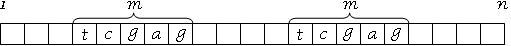
\includegraphics[scale=0.7]{dna-vector.png}
\caption{由N个整数组成的矢量来表示的DNA序列}
\label{fig:dna-vector}
\end{figure}

使用FORTRAN语言编写的解决这个问题的计算机程序如下:

\begin{lstlisting}[language=Fortran]
		DO 10 I = 1,N-M
		DO 10 J = 1,N-M
		FOUND = .TRUE
		DO 20 K = 1,M
20	IF X[I+K-1] .NE. X[J+K-1] THEN FOUND = .FALSE
		IF FOUND THEN ...
10	COUTINUE
\end{lstlisting}

\section{APL}


如果使用APL语言来编写上述这个问题的解决方案,需要重新考虑这个问题。例如,可以把数据重新安排在一个N行M列的矩阵中,而不是前面所使用的由N个元素组成的矢量。

\begin{figure}[htbp]
\centering
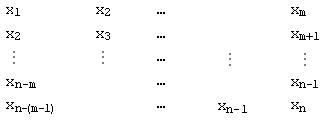
\includegraphics[scale=0.7]{dna-apl.png}
\caption{使用N行M列的矩阵表示DNA序列}
\label{fig:dna-apl}
\end{figure}

把矩阵按行排序(即把一行看作一个单元,在排序过程中移动整行)。如果有任何序列片断被重复,那么在排序后的矩阵中相邻的两行就会有相同的数值。

\begin{table}[htb]
\centering
\begin{tabular}{cccccc}
.&	.&	.&.	&.	&.	\\
T	&G	&G	&A	&C	&C\\
T	&G	&G	&A	&C	&C\\
.&	.&.	&.	&.	&.	\\
\end{tabular}
\end{table}


检查如何满足这项条件很容易。在这里,APL程序之所以快与APL语言本身无关,而是与算法有关。简单的讲,FORTRAN程序使用了一个$O(M\times N^2)$的算法,而APL程序使用的排序方案需要大约$O(M\times N\log N)$次操作。


上述示例的目的并不是说明APL语言在任何情况下,都比FORTRAN语言更有效,而是指APL程序员很自然地被引导发现一种完全不同的解决方式。

虽然使用APL语言很难写循环,而排序却很简单——作为语言组成部分,排序被定义为内部操作符。

在APL语言中,排序运算很容易表达,APL程序员倾向于寻找关于它的创新性应用,这也就说明了解决问题的编程语言是如何引导程序员采用不同的思维方式来看待问题的。

表达思想的语言可以影响或引导思维,这一点在程序设计语言方面得到了很好的体现,因此Spair-Whorf假说认为存在这样一种情况:

\begin{quote}
\texttt{一个生活在某种特定语言环境下的人可能产生或者表达一些想法,这些想法无论如何也无法被生活在另外一种语言环境下的人所翻译和理解。}
\end{quote}

根据Spair-Whorf假说提倡者的观点,这种现象可能发生的情况是在后者的语言中没有对应的词汇或者缺少相关的概念来表达前者的想法。


\section{Turing Machine}

将人类语言产生上述这种现象的可能性与计算机科学中几乎直接对应的计算机语言产生这种现象的可能性相比较是一件有趣的事情,因此逻辑学家Alonzo Church发表了如下的丘奇猜想(Church's Conjecture)。


\begin{quote}
\emph{任何一种具有明确步骤的计算都可以通过图灵机来实现。}
\end{quote}





图灵机是一种可不受存储容量限制的假想计算机,但是图灵机本身是一种极其简单的装置,不需要有很多特性的某种语言来模拟这个装置。

如果我们接受丘奇猜想,那么任何可以模仿图灵机的语言都足以运算任何可实现的算法。为了解决这个问题,首先需要寻找能够生成所期待结果的图灵机。通过丘奇猜想可以知道这种图灵机一定存在,然后用我们所擅长的语言来模拟图灵机的运行。这样关于编程语言相对“能力”的讨论——如果我们把能力理解为“解决问题的能力”——是毫无意义的,而且我们也就陷入了Alan Perlis所提出的“图灵机泥潭”中,这种讨论既无意义又难以摆脱。



需要注意的是,丘奇猜想在某种意义上几乎与Spair-Whorf假说完全对立。


\begin{compactitem}
\item \texttt{丘奇猜想认为在基本方法上,所有的编程语言都是一样的。或者说,一种语言能够表达的想法,在理论上,用另一种语言也能表达。}
\item \texttt{Spair-Whorf假说则认为,存在这样一种可能,某些想法能用一种语言表达,却不能用另外一种语言表达。}
\end{compactitem}

由于无法对“明确的步骤”进行严格的限定,因此天生注定丘奇猜想没有被证实,也无法被证实。不过,至今还没有发现它的反例,似乎可以证明丘奇猜想的可靠性。


人们后来对自然语言提出了一种“图灵机-等价”理论,意思是说,只要通过充分的工作,任何想法都可以用任何语言来表达。

例如,一个一直生活在热带的人无法直觉地用自己的语言对不同类型或用途的雪进行分类,也无法判断雪域的范围,但是只要通过一定时间的培训,就一定能够掌握这种技能。

同样,面向对象技术也不能提供任何新的计算能力,使得原来通过其他方法在理论上无法解决的问题得到解决,但是面向对象技术确实提供了一种方式,使得解决问题更加容易和自然,而且这种方式有效地改善了大型软件项目的管理。


无论是计算机语言还是自然语言,语言只能引导思维,而不能阻止思维。面向对象编程不仅仅是在编程语言中加入一些新的特征,更重要的是,它是用来分析处理问题和开发计算机程序解决方案的一种崭新的思考方式。

可以肯定地说,一个由具有共同兴趣的个体组成的群体,倾向于发展他们自己的特殊词汇,一旦这些词汇形成,它们就会影响这些人的思维方式,而对于群体以外的人,这种方式很难理解,这本身就是一个OOP的实例。

既然面向对象思想在一定的原则下不需要面向对象语言就可以使用,那么面向对象术语的使用就能够帮助用户以一种对于没有OOP术语的人来说也能理解的方式去思考问题。


\chapter{Real World}

下面首先考虑一下我们如何处理现实世界的情况,然后再去考虑在使用计算机解决问题时如何应用这种技术模式。

假设有一位名叫Chris的人想送花给他的一位叫Robin的朋友,Robin生活在另外一个城市。因为距离太远,Chris不能亲自把花送给他的朋友。不过,可以通过别的办法来完成。Chris来到附近的一家花店,这家花店由一个名叫Fred的花商经营。Chris把打算送给Robin的花的种类和Robin的地址告诉给Fred。这样Chris就可以确信他的花可以方便地送到他的朋友那里了。

\begin{figure}[htbp]
\centering
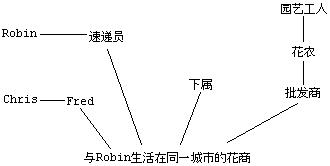
\includegraphics[scale=0.65]{flower.png}
\caption{现实世界中的实例}
\label{fig:flower}
\end{figure}

这里解决问题的方法就是找到一个合适的代理(也就是Fred),并且把自己的要求告诉他。代理有责任完成这些要求,Fred会选择某种方式——一种算法或一系列操作——来完成这项任务。Chris没有必要了解Fred使用什么方法来完成任务。实际上,使用代理的人通常不想了解完成任务的细节,这些细节一般都是隐蔽的。

通过调查可以发现,Fred向一位与Robin生活在同一城市的花商传递了一条信息,然后,那名花商可能会让一名下属来安排这件事。接着花和另外一条消息将交给一个速递员。这样依次进行下去。此时我们又会发现,与Robin生活在同一城市的那个花商一直都从花卉批发商那里购进花。同样地,花卉批发商又与花农交易,而花农则要管理园艺工人。

由此,我们得到关于通过面向对象思想解决问题的初步结论:解决问题需要很多其他个体的帮助。没有这些个体的帮助,问题难以解决。简单概括如下:

\begin{quote}
\emph{一个面向对象程序可以由一个团体(集合)组织而成,这个团体由一组互相作用但又松散连接的叫做“对象”的代理组成。每一个对象都扮演一个角色,对特定的任务负责,并且为团体中的其他成员提供特定的服务或者执行特定的行为。}
\end{quote}

设计一个面向对象程序就像组织一个团体,团体中的每个成员都被赋予一定的责任,这样程序功能的实现就来自其中每个对象的努力及它们之间的相互协作。

\section{Message}

开始,Chris向花商Fred提出要求,此项要求导致了另外一项要求,然后又继续导致更多的要求,直到花最终送到Chris的朋友Robin手中。

通过这一系列的连锁反应,Chris的要求最终被实现了,而且由此可以看到,团体的成员通过传递要求来相互协作。

下面提出的通过面向对象思想解决问题的原则是确定传递工具来指示下一步行为。

\begin{quote}
\textbf{在面向对象编程中,行为的启动是通过将“消息”传递给对此行为负责的代理(对象)来完成的。}

\textbf{消息对行为的要求进行编码,并且伴随着执行要求所需的附加信息(参数)来一起传递。“接收器”就是接收消息的对象。}

\textbf{如果接收器接收到了消息,那么同时它也接受了消息所包含的行为和责任,然后接收器响应消息,并执行相应的“方法”以实现要求。}
\end{quote}

与消息传递相关的是信息隐蔽原则——提出要求的客户不需要了解实现该要求的具体方式,还有另外一条原则——我们所知道的所有人都是隐藏在消息传递过程中的。客户如果要完成一项任务,首先的想法就是寻找能够执行这项任务的人。


面向对象编程的一个重要部分就是可复用组件的开发。使用可复用组件的第一步,也是非常重要的一步,就是程序员能够接受、信任他人编写的软件。在实际的计算机解决方案中,最终是通过对象的相互作用来完成计算的。

在传统的语言中,信息隐藏(information hiding)也是编程的一个重要方面。虽然根据要求两者都会运行一系列预定义的步骤,但是它们也有两点截然不同的地方。

\begin{description}
\item[首先] 每一条消息都与一个指定的接收器相对应,接收器就是接收消息的对象。过程调用却没有指定的接收器。
\item[其次] 消息的解释(即用于响应消息的方式)由接收器来决定,并且随着接收器的不同而不同。
\end{description}

例如,Chris给他的一位名叫Elizabeth的朋友发了一条消息,她接收到消息之后,立即采取了相应的行动(即把花送给了他们共同的朋友Robin)。但是,Elizabeth完成要求的方法和Fred完成相同要求的方法是完全不同的。

如果Chris让牙医Kenneth将花送给Robin,而Kenneth可能没有办法解决这一问题。如果他完全理解了这个要求,则有可能向Chris返回一个信息来说明错误。

从上述可以得出,消息传递与过程调用有如下的区别:

\begin{quote}
\texttt{消息传递有一个指定的接收器,解释——选择响应消息的方法——可能因接收器的不同而不同。}
\end{quote}

通常,人们在程序运行之前不会知道任何消息的接收器,也不会知道调用了哪些方法。

一般情况下,消息(函数或过程名称)和响应消息的代码段(方法)之间是后期绑定的关系。与之对应的是,传统过程调用中名称与代码段之间的早期(编译时或链接时)绑定关系。

\section{Responsibility}


面向对象编程的一个基本概念就是用责任来描述行为。例如,Chris对行为的要求仅仅表明他所期望的结果(把花送给Robin)。Fred可以任意选择使用的方法来实现所期待的目标,并且在此过程中不会受到Chris的干扰。

通过用责任来讨论问题,提高了问题抽象的水平,使得对象之间更加独立,这正是解决复杂问题的关键。通常用协议来描述与一个对象相关的所有责任的集合。

传统程序的执行通常是通过对数据结构进行操作——例如,改变数组或记录中的域。与此相反的是,面向对象程序则要求数据结构(即对象)提供服务。


从传统的、结构化数据的角度来观察软件与从面向对象的角度来观察软件之间的区别,可以得到下面的结论:

\begin{quote}
\emph{不要问你能为数据结构做什么}

\emph{要问数据结构能为你做什么}
\end{quote}

\section{Class}

在上述示例中,Chris对Fred提出送花给Robin的要求之后,他大致上可以认定这个事件会发生在Fred的花店里。Chris做出这样的假定是基于以往同其他花商打交道的经验,因此Chris认为Fred作为这一类别中的一个实例,应该适用普遍的模式。

这里。我们可以用花商来代表所有花商中的一个类别(或者是类),从而可以把这些概念总结成面向对象编程的另外一个原则:

\begin{quote}
\emph{所有对象都是类的实例。}

\emph{由类的接收器来决定在响应消息时调用的方法。}

\emph{一个特定类的所有对象使用相同的方法来响应相似的消息。}
\end{quote}

对象是对状态(数据值)和行为(操作)的封装,因此对象和专用计算机有很多相似之处。

\begin{compactitem}
\item 对象的行为由对象类来规定。
\item 每个对象都是某个类的一个实例。
\item 同一个类的所有实例都以相似的方式(即调用同一方法)来响应相似的要求。
\end{compactitem}





对象通过调用方法表现其行为(类似于执行一个过程),并以此来响应消息。对消息(即所使用的特定的方法)的解释由对象决定,并且随着对象类的不同而不同。



\section{Inheritance}

Chris还有Fred更多的信息——这不仅是因为他是一个花商,更是因为他是一个店主。例如,Chris知道钱的转移是这项交易的一部分,同时作为付款的凭证,Fred交给Chris一张收据,而这些行为同样也会发生在食品商、文具商和其他店主身上。由此可知,花商这个类别是店主类别的一个特殊类别。Chris知道,关于店主的一切对于花商也同样适用,于是这也适用于Fred。

下面将讨论Chris是如何组织关于Fred的信息的,我们可以通过分类层次来考虑。Fred是一个花商,而花商又是店主的一种特殊形式。进一步讲,店主是一个人。而Chris知道所有关于人的一切也同样适用于Fred,尽管这些信息没有直接与他发生联系。


一般类别的信息也适用于特殊类别,这样的原则称为继承。

通常情况下,可以利用一种交错的图像技术来说明继承关系(尤其是当很多个体有不同的归属时),通过继承技术可以把类组成树状层次结构。其中,继承结构中的比较抽象的类位于树的顶端,比较具体的个体位于树的底部。

\begin{quote}
\texttt{类可以组织成一个有层次的继承树结构。}

\texttt{子类继承层次树中更高一层的父类的属性和行为。}

\texttt{抽象父类不能有具体实例,只能用来产生子类。}
\end{quote}


继承的引入使得树中较低层次的类可以存取和使用与树中较高层次的类相关的数据和行为。


\section{Override}

为了解决类的层次结构中平行类的相关问题,需要寻找一种技术,能够处理一般规则以外的特例。

我们可以通过在子类中发布一条信息来解决此问题,这条信息可以改写(override)从父类继承的信息。通常,给子类中某一方法取一个与父类中某一方法相同的名称,再结合寻找方法的规则(当响应特定信息时)来实现这个目的。

\textbf{接收器类搜索并执行相应的方法以响应给定的消息。如果没有找到匹配的方法,搜索就会传导到此类的父类。搜索会在父类链上一直进行下去,直到找到匹配的方法,或者直到父类链结束。}

\begin{compactitem}
\item \textbf{如果是前一种情况,就会执行方法;}
\item \textbf{对于后一种情况,会产生错误信息。}
\end{compactitem}

\textbf{如果能在更高类层次找到相同名称的方法,所执行的方法就称为\textcolor{blue}{改写}了继承的行为。}

虽然编译器在运行时不能确定调用哪个方法,但是许多面向编程语言能够确定是否有合适的方法以供调用,并且能够产生错误信息作为编译时错误诊断,而不是运行时信息。

不同的对象都会对类的消息做出相应的反应,但执行的方法却不同,这也就是多态(polymorphism)的一种表现。

例如,Elizabeth和Fred都会对Chris的消息作出反应,只是执行的方法不同,而且Chris不了解也不需要确切地了解Fred使用的方法,从而也对信息进行了有效的隐藏。

\chapter{Metaphor}



计算机执行程序的行为的模型是一个过程状态或者鸽子窝模型,或者说,计算机是一个数据管理员,跟随着一些指令模式,在存储器中从不同的槽(内存地址)中取出数值,用某种方式对它们进行转换,再将结果推入到另外的槽中。检查槽中的数值就可以确定机器的状态或者计算的结果。

虽然这个模型与实际计算机内部的工作流程大致吻合,但对于我们理解如何使用计算机来解决问题,却没有多少帮助,而且这也不是我们大多数人解决问题的方式。

在面向对象框架中,用户几乎不提内存地址、变量、赋值或者任何传统编程术语,只是使用对象、消息和某种行为的责任。

在面向对象编程思想中,用户拥有的是一组行为规范的对象,各个对象之间通过礼貌地交互来实现各自的愿望。


在很多方面,把编程比作创建“域”的观点和一种称为“离散事件驱动模拟”的计算机模拟很相似。简而言之,在离散事件驱动模拟过程中,用户为不同的模拟元素创建其计算机模型,通过模型来描述元素之间如何相互作用,并使它们运作起来,这几乎等同于通常的面向对象程序。

在通常的面向对象程序中,用户需要描述域中的不同实体代表什么、它们如何相互作用以及如何使它们最终运作起来,因此我们可以得到下面这样的结论。

\begin{quote}
\textbf{在面向对象编程中,计算就是模拟。}
\end{quote}

面向对象编程把程序看成是一个集合,这个集合由称为对象的松散连接的代理组成。

\begin{compactitem}
\item 每个对象都对特定的任务负责。
\item 通过对象的相互作用进行计算。
\end{compactitem}

从某种程度上说,编程就是一个对模型域的模拟。通过类和模拟的概念,初学者可以更容易地理解隐喻(metaphor)。

隐喻有利于面向对象技术的应用,但是通常它却很容易被忽略。例如,当用户根据对象的行为和责任思考问题时,可以为用户带来很多的关于日常经验的直觉、思想和理解力。

如果把问题想象成鸽子窝、邮箱或者包含数值的槽时,用户几乎不需要什么背景知识就可以深入了解问题并对其结构化,这些都是隐喻的强大的解释力量的反映。

不同于以往的编程方法,使用面向对象编程思想分析问题和编写程序解决问题时,为开发者提供了更大的构件,开发者通过迅速地用它们组装自己的软件就可以解决问题,这一方面可以类比Lego玩具提供的各种组件。

通过减少软件组件之间的相关性,面向对象编程可以实现可复用软件系统的开发。

可复用的组件与软件应用的其他部分是隔离的,从而可以作为独立的单元来创建和测试,而且可复用的软件组件允许用户在更高的抽象层次上处理问题,这样就可以简单地通过能被对象所理解的消息和对象需要执行的任务来定义和操作对象,而不必考虑执行细节。

当然,对象不可能总是通过礼貌地请求另一个对象执行某种行为来响应消息。如果这样,结果会形成一个无限的请求循环,就像两个绅士都礼貌地等待另一位先进门,或者像一个使用纸上签字的官僚机构,每一个人都把所有的待签纸传给组织中的另外的人。

在某种程度上,至少有几个对象,除了传递请求给其他代理之外,还执行一定的工作。根据所使用的面向对象语言的不同,这项工作的完成情况也不同。

\begin{compactitem}
\item 面向对象/命令的混合语言(如C++语言、Object Pascal语言和Objective-C语言)通过基础(非面向对象)语言编写的方法来完成。

\item 更加纯粹的面向对象语言(例如Smalltalk或者Java)是通过语言基本体系结构所提供的“原始的”或者“固有的”运算指令来完成。
\end{compactitem}

另外,Peter Wegner提出了区别基于对象语言和面向对象语言的不同之处的方法,基于对象语言只支持抽象(如Ada),而面向对象语言还必须支持继承。

\begin{quote}
\texttt{Apple Object Pascal语言最初是由Larry Tesler定义的,Borland Pascal语言最终演化成了Delphi语言。Objective-C语言的创建者是Brad Cox,在它作为C语言的扩展语言产生的同时,C++语言也开发完成,Smalltalk语言也有其公共流行版本Squeak。}
\end{quote}

\chapter{Abstraction}

在打开一本地图册时,首先会看到一张世界地图,而且其中只会显示某些最重要的特征,例如各种山脉、河流和其他一些非常大的建筑物,一些细小的特征都被忽略了。

随后的地图会描绘出一些小的地理区域(通常还有更多的细节),例如:

\begin{compactitem}
\item 一个洲的地图可能包括政治边界和一些主要的城市;
\item 一张关于更小区域的地图(例如一个国家)可能包括城市、乡村和更小的地理特征,比如某个山脉的名称;
\item 一张大城市的地图可能包括出入城市的主要道路;
\item 比城市更小的区域地图甚至可能标注出每一座建筑。
\end{compactitem}

在每一级别水平上都会包括某些特定的信息,而故意忽略了某些其他的信息。当以更高级别的抽象来看待一件制品时,没有什么方法能够描述它的细节。

即使能够描述出这些细节(比如用极小的字),人们也无法吸收或处理如此大量的信息,因此一些细节就这样简单地被忽略了。

通常,人们只使用几种简单的工具去创建、理解和管理复杂的系统,其中抽象就是最重要的技术之一。

\begin{quote}
\texttt{抽象(abstraction)是指对于一个过程或者一件物品的某些细节的有目的的隐藏,以便把其他方面、细节或者结构表达得更加清楚。或者说,抽象就是为了强调指定的特征而有目的地压缩细节。}
\end{quote}



用户通过抽象可以建立起针对实际系统的不同层次的模型,因此抽象通常与组件划分相联系。

在形成抽象或模型时,需要有意识地避免理解很多细节,并且集中精力在几个主要特征上面,因此经常使用另外一个术语来描述这样的行为:信息隐藏。

\begin{quote}
\texttt{信息隐藏描述了部分抽象,通过它就可以有意地忽略某些特征,以便于能够集中强调其他特征。}
\end{quote}

抽象产生的组件封装(encapsulate)了某些主要特征,并通过简单和固定的接口(interface)与其他组件进行相互。

\section{Abstraction Level}


在一个典型的面向对象程序中,有很多抽象层次。

\begin{compactitem}
\item 更高层次的抽象体现了面向对象程序的特征。
\item 在最高层次的抽象层次上,程序被看作是一个由很多对象组成的“团体”。
\end{compactitem}


\begin{figure}[htbp]
\centering
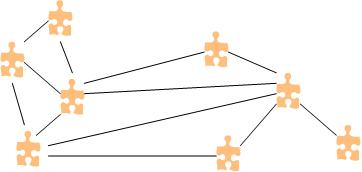
\includegraphics[scale=0.6]{abstract-level.png}
\caption{抽象层次}
\label{fig:abstract-level}
\end{figure}


在面向对象开发中,团体这个概念有两种不同的形式,而且信息隐藏和抽象等面向对象思想对这两种形式都适用。

\begin{compactitem}
\item 程序员团体

在现实世界中,为了完成应用程序,程序员之间必须互相合作。
\item 程序员创建的对象团体

在虚拟世界里,对象之间必须互相合作来实现共同目标。
\end{compactitem}



团体中的每一个对象都为组织中的其他成员提供服务,在最高级别的抽象层次上需要强调的最重要的特征就是交流和合作的通道,以及成员之间相互合作的方式。

下一个级别的抽象不会在所有的面向对象程序中出现,也不被所有的面向对象语言所支持。但是,很多语言都允许一组对象一起工作,形成一个单元(unit)。

关于这个思想的实例有Java语言中的包(packages)、C++语言中的名称空间(name spaces)和Delphi语言中的单元(units),这样就允许某些特定的名称暴露在单元以外,其他的特征则隐藏在单元内部。

\begin{quote}
\texttt{实际上,单元的概念继承了C和Modula等语言中的模块(module)思想,面向对象编程思想应归功于早期的模块研究。}
\end{quote}


下面两个级别的抽象是用来处理两个独立对象之间的交互。例如,我们常说的是一个对象能够为其他对象提供服务,这种直觉的建立来自于对客户和服务器之间通信的描述。

这里的服务器只是表示提供服务的对象,而且这两个层次的抽象涉及了对这种关系的两种视角,一种来自于客户端,一种来自于服务器端。


在一个优秀的面向对象设计中,我们可以描述和讨论服务器所提供的服务,而无需提及客户在使用这些服务时可能执行的任何行为。

下面可以把关于信息隐藏和抽象的表述想象成一个描述了数据结构(如堆栈)所提供的服务的广告牌。


\begin{figure}[htbp]
\centering
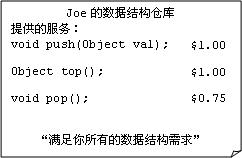
\includegraphics[scale=0.6]{ad-board.png}
\caption{广告牌}
\label{fig:ad-board}
\end{figure}

高级别的抽象通常用接口来表示,实际上接口是一个与类相似的结构,它定义了行为,但不描述如何来实现这些行为。

\begin{lstlisting}[language=Java]
interface Stack{
	public void push(Object val);
	public Object top() throws EmptyStackException;
	public void pop() throws EmptyStackException;
}
\end{lstlisting}


下一抽象层次查看同一边界,但却不同于服务器端。这里的抽象层次需要考虑抽象行为的具体实现。例如,有很多数据结构可以用来满足堆栈的要求,这样的抽象层次主要关注服务的具体实现方式。

\begin{lstlisting}[language=Java]
public class LinkedList implements Stack ...{
	public void pop()	throws EmptyStackException{...}
	...
}
\end{lstlisting}


在抽象的最底层需要单独考虑一项独立的任务(即一个方法),因此这一层次的抽象主要关注的是执行这一活动所需操作的精确顺序。例如,我们可能需要研究用来移走放入堆栈里的最近元素的操作。

\begin{lstlisting}[language=Java]
public class LinkedList implements Stack ...{
	...
	public void pop() throws EmptyStackException{
		if(IsEmpty())
			throw new EmptyStackException();
		removeFirst(); //delete first element of list
	}
	...	
}
\end{lstlisting}

在软件的开发过程中,每一个抽象层次在某些方面都很重要。实际上,程序员需要在各种抽象层次之间迅速地移动,也就要求在每一个抽象层次上执行相应的面向对象的分析。

在软件开发的早期,一个关键的问题就是如何确定正确的抽象级别,通常出现的错误是在低层次的抽象级别上反复思考,担心各种关键组件的实现细节,而不是努力地思考如何实现高级别的抽象来促进有关问题之间的完全分离。

在软件开发过程中的任何时刻,程序员(或开发一个比较大的项目的设计小组)都必须进行缜密的思考,才能确定正确的抽象级别。

对于特定问题,人们通常不愿忽略或者放弃很多的细节,但是实际上不能过多地关注细节,否则一些重要的问题就会被掩盖。


\section{Abstraction Pattern}

抽象可以用来帮助理解复杂的系统,从而反映出系统某些真实的方面,或者它可能只是一种思维的抽象,用来帮助我们理解真正的问题。

在某种程度上,抽象是系统结构的版图。

抽象的思想可以进一步划分为不同的形式,通常的技术是将一个层次划分成各种组成部分。例如,当我们描述汽车是由发动机、传动装置、车体和车轮组成时,所使用的正是这个方法。

下一个理解层次是通过依次检查每一个组成部分来实现,这不过是分而治之(divide and conquer,分治法)的一个体现。

\begin{figure}[htbp]
\centering
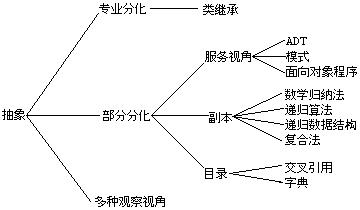
\includegraphics[scale=0.6]{abstract-pattern.png}
\caption{抽象的其他形式}
\label{fig:abstract-pattern}
\end{figure}

有时候我们使用不同类型的抽象,因此另外一种形式就是特化分层思想。

例如,对于汽车的理解就可以部分基于以下知识。首先,它是一个有轮子的车辆,其次,它是一种交通运输工具。

当我们还了解其他一些关于有轮车辆的知识后,这些知识既适用于汽车,也适用于自行车。如果还了解其他各种不同的运输工具,这些知识也可以同样地适用于驮马,也适用于自行车。

面向对象编程语言广泛地使用特化分层的抽象形式。

\begin{figure}[htbp]
\centering
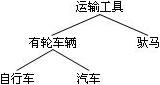
\includegraphics[scale=0.6]{abstract-example.png}
\caption{特化分层}
\label{fig:abstract-example}
\end{figure}

部分分化和专业分化的思想代表了在面向对象编程中使用的两种最重要的抽象形式,即通常所说的“是抽象”和“有抽象”。

\begin{description}
\item[是抽象]

专业分化是指“是抽象”,例如自行车“是有轮车辆”,它“又是运输工具”。

\item[有抽象]

部分分化就是“有抽象”,例如汽车“有发动机”。
\end{description}

在实际的计算机程序设计过程中,“是抽象”和“有抽象”会与特定编程语言的特征联系在一起。

人们最常使用的用来帮助理解复杂系统的技术就是把抽象和分化成的各种组件结合起来。

我们对汽车的描述就是一个这样的例子,理解下一个层次需要通过对每一个组成部分进行更精细的细节分析来实现。例如,对汽车发动机更精细一些的描述,就是把它看作圆柱体的组合,每一部分都能将燃料的爆炸转变成垂直方向的运动,并通过曲轴将圆柱体的上下运动转换成旋转运动。

另外一个例子是关于如何组织人体运动的信息。在某一层次上,我们只关系各种组织,把人体看作是由骨骼(保持刚性)、肌肉(产生运动)、眼镜和耳朵(产生感觉)、神经系统(传递信息)和皮肤(把各个部分连接起来)组成的。在下一个抽象层次上,我们可能会考虑肌肉是如何工作的,并且会考虑一些比如细胞结构和化学作用的问题,而化学作用又是由分子结构决定的。为了了解分子,又得把分子继续分解为原子。

任何解释都必须基于正确的抽象层次来阐述,因此如果试图以原子层次的细节来解释一个人是如何行走的,将会是极其困难的。


\section{Encapsulation}


创建一个大系统的关键步骤就是将其分成合理的组成部分。

实际上,不管是编写软件还是建造汽车,通过将整体的大的系统进行合理的划分,就可以分配人员基本独立地进行各部分的工作。



封装的基础是内部视角和外部视角之间有着严格的区分,因此制造发动机的小组成员对传动装置只需要有一个抽象的(也就是外部的)理解,而制造传动装置的小组成员则需要对传动装置具备详细的内部理解。

封装允许用户考虑实现互换的可能性,当把一个系统划分为几个部分时,理想的目标就是将各个部分之间的相互作用减少到最少。例如,通过封装发动机的行为可以与传动装置隔离,从而可以把一种类型的发动机转换成另外的类型,不会影响系统其他部分的运行。

为了将这些思想应用于软件系统,用户需要一种方式来讨论软件组件执行的任务,而且这种方式要和组件满足责任的方式区别开来。


\section{Interface}

在软件系统中,使用接口和实现这两个术语来描述一项任务包含哪些内容和如何实现任务,以及外部视角和内部视角之间的区别。

\begin{compactitem}
\item 接口描述系统被设计用来做什么,这是抽象使用者必须理解的思想。
\item 接口并没有说明所分配的任务应如何执行。
\item 接口通过与完成抽象的实现相匹配来使系统正常工作。
\end{compactitem}

在汽车工业中,发动机的设计者会与传动装置的接口相联系,而传动装置的设计者必须实现这些接口。

同样地,开发复杂的计算机软件系统的一个重要步骤就是将一项任务分成几个部分,这些部分可以由小组的不同成员来开发。其中,每一个部分都有两个方面:接口显示给外部世界,而实现用来完成接口的要求。

接口和实现的分离不但使得在较高层次上理解一项设计更加容易(因为接口的描述比任何特定实现的描述都简单得多),而且使软件组件的互换性成为可能(因为可以使用任何实现,只要它能够满足接口规范)。

\begin{quote}
\textsl{当一个系统中组件的数量越来越多的时候,以“目录”的方式来组织它们通常是很有效的。}
\end{quote}

在日常生活中我们要使用很多不同形式的目录。例如,电话号码簿、字典或搜索引擎等。类似地,在软件中也使用各种各样的目录,一份关于系统中所有类的简单列表就是一个这方面的例子。

另外一个目录的例子就是由类所定义的所有方法组成的清单,例如Java标准库的类参考手册就是一个非常有用的目录。

\begin{quote}
\textsl{目录为用户提供了一种机制,使用户可以从一个范围很大的集合中迅速地定位到某一特定的位置(可以是类、对象或者方法)。}
\end{quote}


接口描述了软件组件所提供的服务,但是不必描述完成服务所使用的技术,这个思想是理解和处理复杂软件系统的核心手段。例如,在上述关于送花的实例中,强调的也是这种抽象,而且这个实例的最后结果是有很多人都参与了送花的过程,并且在每个流程都各司其职。

\begin{figure}[htbp]
\centering
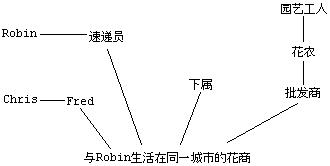
\includegraphics[scale=0.6]{interface-service.png}
\caption{服务视角}
\label{fig:interface-service}
\end{figure}


团体中的每个成员为这个团体中的其他人提供服务,没有一个成员能够自己独立地解决问题,只有通过互相协作,才能实现所期待的结果。




\section{Compounding}


复合法是另外一种从独立的部分创建复杂结构的强大技术。这一思想从少量几个基本的形式开始,然后增加一些规则,将各个形式结合起来创建新的形式。


\subsection{Regular Expression}


复合法的主要原则是允许合并机制,既可以作用于新形式也可以用在原来的基本形式上。例如,正则表达式(regular expression)就充分地说明了复合法技术。

正则表达式是描述一系列数值的简单技术,它的描述是从确认基础的字符表开始的。

以字符a、b、c和d为例进行说明,任何单独字符的例子都是一个正则表达式,然后我们可以增加一条规则,即由两个正则表达式组成的复合结构也是一个正则表达式。

\begin{lstlisting}[language=bash]
abaccaba
\end{lstlisting}

通过反复地应用复合法规则,就可以发现任何有限的由字符组成的字符串都是正则表达式。



下一个合并规则是说两个正则表达式的可替换形式(用竖线“|”来表示)是一个正则表达式。正则表达式遵循这样的运算规则,复合运算优先于可替换运算规则,因此下面的模式代表一系列由三个字母组成的值,由ab开始,并以a、c或者d结束。

\begin{lstlisting}[language=bash]
aba|abc|abd
\end{lstlisting}

如果可以用括号来表示分组,就还可以表示成下面的形式:

\begin{lstlisting}[language=bash]
ab(a|c|d)
\end{lstlisting}


最后,符号“*”(通常称为星号)用来表示“0或者多个重复”的概念,把这些规则结合起来就可以描述非常复杂的字母组合。

例如,下面一系列字符值的描述是以a或者b的循环紧接着一个c来开始,或者是以dd两个字母序列开始,然后是字母a。

\begin{lstlisting}[language=bash]
(((a|b)*c)|dd)a
\end{lstlisting}

\subsection{Type System}


\begin{quote}
\textbf{复合法的思想也是类型系统的基础。}
\end{quote}

类型系统始于原始类型(例如整数类型和布尔类型),类的思想允许用户创建新的类型,这些新的类型可以包含从前一类型构建出的数据字段。

这里的前一类型可能是原始类型,也可能是用户自定义的数据类型。既然可以以先前所定义的类为基础来创建类,那么就可以逐渐地构建出非常复杂的系统。


\begin{lstlisting}[language=Java]
class Box{ // a box is a new data type
	...
	private int value; // built out of the existing type int
}
\end{lstlisting}



\subsection{GUI Library}

复合法原则还有另外一项应用,就是便于进行窗口布局的用户界面控件库。

窗口是由一些简单的数据类型(例如按钮、滑块和绘图板等)组成的,各种类型的布局管理器都要创建一些简单的结构。例如,一个网格布局定义了一个矩形网格,每个网格的大小相同,边界布局管理器确定了这样一种规范,允许5个组件分布在屏幕的北、南、东、西和中各个部位。

\begin{figure}[htbp]
\centering
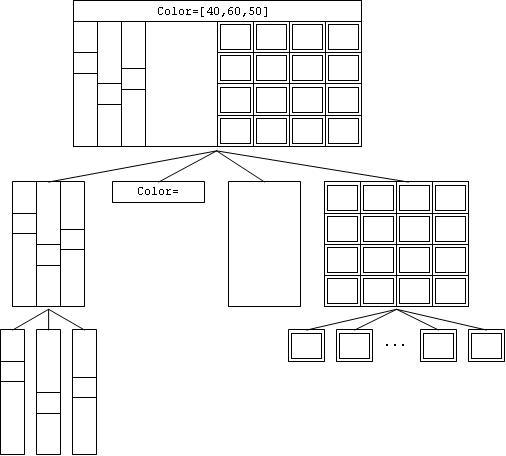
\includegraphics[scale=0.4]{compound-window.png}
\caption{复合窗口}
\label{fig:compound-window}
\end{figure}

和正则表达式一样,窗口也可以作为其他窗口的一部分。例如,如果要定义一个窗口,左边有3个滑块,中间有一个绘图板,16个按钮4个一组地依次排列在右边,文本框排列于顶部。我们通过把简单的窗口放置在较为复杂的窗口中,就能够实现这一需求。




大多数计算机程序本身就可以看成是复合的产品,这时方法或者过程的调用就是复合的机制。

实际上,从语言的基本语句开始(赋值等),通过复合法可以建立一个实用的函数库。以这些函数库为基础,就可以形成更加复杂的函数。如此继续下去,每一层都建立在上一层的基础之上,直到最终完成所要求的应用程序。

抽象通常与组件(component)划分相联系,组件封装了某种主要特征,并通过简单和固定的接口(interface)与其他组件相互作用。

组件的划分意味着我们可以把一项大任务分成一个个的小问题,这样这些小问题就可以大体上相对独立地进行解决,提供符合接口要求的实现(implementation)是每一个组件开发者的责任。

\section{Specialization}



另外一个处理复杂问题的方法是使用特化分层来构建抽象,有时也把它称为分类系统。例如,在生物学上把生物分为动物和植物,动物又分为脊椎动物和无脊椎动物,脊椎动物包括哺乳动物,哺乳动物包括狗、马、鲸鱼等。

\begin{quote}
\texttt{这种分类同时也存在特例,鸭嘴兽是产蛋的哺乳动物,因此如果我们把这种特殊现象与哺乳动物生产幼仔来繁衍后代的特征相联系,就需要更改鸭嘴兽的特征来解释为什么鸭嘴兽属于哺乳动物,却能够产蛋的事实。}
\end{quote}






面向对象语言也需要一种特化分层机制,来改写从更加普遍的类别继承而来的信息,这就需要更加深入地讨论类继承的思想。

使用特化分层抽象与以前的抽象之间的主要区别在于越特化的抽象层次是越普遍化的抽象层次的表现。不过,与前面所使用的从肌肉的特性抽象到各种化学作用的描述时的观点是不同,因此这两种不同的关系可以描述成是(is-a)继承关系和有(has-a)继承关系。

实际上,使用任何一种抽象类型的原因都是一样的。抽象的原则允许我们忽略某些细节,以便更易于表现少数几个主要的特征。



同样的技术也应用在面向对象语言,新的接口从现有的接口上形成。一个类从已有的类那里继承而来,这时和原始类相关的所有特性(数据字段和行为)都同样适用于新类。




在Java AWT(Abstract Windowing Toolkit)库的案例中,当使用AWT创建一个新的应用程序时,主类作为Frame的子类,依次地和AWT库的其他类链接。

\begin{figure}[htbp]
\centering
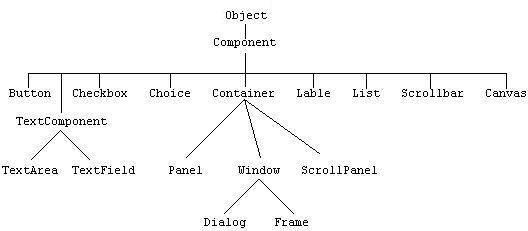
\includegraphics[scale=0.5]{awt-example.png}
\caption{Java AWT类层次}
\label{fig:java-awt-example}
\end{figure}

Frame是应用程序窗口的一种特殊类型,但是它也是Window类的一种更特殊的形式。Window可以包括其他的图形对象,因此它也是一个Container类型。

每一个继承层次都为更低的层次提供方法,即使最简单的应用也需要使用如下的方法。

\begin{table}[htbp]
\centering
\begin{tabular}{ll}
setTitle(string)	&从类Frame继承而来\\
setSize(int,int)	&从类Component继承而来\\
show()			&从类Window继承而来\\
repaint()			&从类Component继承而来\\
paint()			&从类Component继承而来,将在新的应用程序中被改写\\
\end{tabular}
\end{table}



分类系统——在面向对象语言中更倾向于使用继承层次(inheritance hierarchy)这个术语。其中,层次是一个普通类别的更详细的表示,每一层次都是上一层次更加特殊的表现。例如,一个类型系统的例子就是生物学上的分类,其中更一般层次的知识适用于那些更特殊层次的对象。

如果将继承层次技术用于软件系统时,可以大大简化新组件的创建。

\begin{compactitem}
\item 新组件和已有的类别相关;
\item 新组件可以自由地利用已有类别的所有功能(例如Java类库中的Frame组件)。
\end{compactitem}


\chapter{Pattern}

当面对一个新问题时,大多数人会首先看一看他们曾经解决过的问题和现在的新任务有什么共同的特征,因此那些原来的问题可以作为一种模式,新问题也将以相似的方式进行处理,只需针对不同的环境做一些必需的改动,这一观察结果暗示了软件模式(Pattern)的思想。

\begin{quote}
\textsl{模式就是试图为问题提出一个已经被证实的解决方案,以便于能够很容易地用类似的方式来解决以后的问题。在面向对象领域,这一思想广泛地用来描述对象团体中成员之间的相互作用模式。}
\end{quote}

下面用一个简单的例子证明模式的这一思想。假设正在开发一个网络应用程序,这意味着应用程序的一部分运行于一台计算机,另一部分运行于通过网络连接着的另外一台计算机。在这两台计算机之间建立实际的连接和通过连接传递信息这些细节,可能与应用程序的大部分应用都毫不相关。

构建上述这些关系的一种方式就是使用一种称为代理的模式,代理是一种将网络连接隐藏于其中的中介。

对象可以和代理相互作用,但却完全感觉不到代理内部使用哪种具体的网络连接类型。当代理接收到一项关于数据或者行为的请求时,它把这些请求打成一个包,通过网络进行传输,然后接收到响应包,解包,再将响应信息返回给客户。

通过代理模式完成客户请求时,实际上客户完全感觉不到网络协议的细节。
\[\mbox{\fbox{客户}}\longrightarrow \mbox{\fbox{代理}} \longrightarrow \mbox{\fbox{服务器}}\]

需要注意的是,这种模式的描述是如何抓住交互的关键点(对客户隐藏通信协议的需要),而忽略交互的其他方面的(例如在客户和服务器之间传递的特定的信息)。

\begin{quote}
\textsl{模式是对某些已经在多个地方、以多种形式出现过的问题的解决方案的概括性的描述,说明了如何确定问题,同时解释了采用某种解决方案和考虑其他替代方法的原因。}
\end{quote}




\chapter{Language}


面向对象技术并不是革命性地,它只是从模块到抽象数据类型最终到对象这个发展过程地自然结果,因此从汇编语言到面向对象编程语言的本质都是抽象机制。



\section{Assembly}





在使用机器语言进行编程时,存储单元使用地址进行描述,无法按照名称或目的来描述。

类似地,运算使用数字操作码进行描述。例如,整数加法使用操作码33,整数减法使用操作码35。


下面的示例把地址372中的内容加到地址376中的内容上,然后从结果中减去地址377中的内容。

\begin{lstlisting}[language=bash]
33  372  376
35  377  376
...  
\end{lstlisting}


相比机器语言,汇编语言允许使用符号名称,因此可以使用汇编语言对上述示例进行改写。

\begin{lstlisting}[language=bash]
ADDI  A, X
SUBI  B, X
...
\end{lstlisting}


汇编语言本身是对机器语言的抽象,而且汇编语言和过程作为抽象机制把用户的视角集中在功能层次上——如何完成一项任务,从而使编程更加人性且友好。


\section{Procedure}

过程和函数代表编程语言抽象的进一步改进。其中,过程提取重复执行的任务的定义用以复用,而且过程还为信息隐藏提供了可能,这样其他用户就可以通过接口来调用过程,无需了解其实现的确切细节。

下面以堆栈为示例进行说明,首先需要建立工作的可视接口(即init、push、pop和top例程),然后确定合适的实现技术(例如包含栈顶指针的数组、链表等)。



\begin{lstlisting}[language=C]
int datastack[100];
int datatop=0;

void init(){
	datatop=0;
}

void push(int val){
	if(datatop<100){
		datastack[datatop++]=val;
	}
}

int top(){
	if(datatop>0){
		return datastack[datatop-1];
	}
	return 0;
}

int pop(){
	if(datatop>0){
		return datastack[--datatop];
	}
	return 0;
}
\end{lstlisting}

在使用过程来实现上述例程时就会发现,4个例程中的任何一个都不能局部创建堆栈本身所包含的数据,它们必须共享这些数据。如果选择只能是局部变量或者全局变量,那么堆栈数据只能保存在全局变量中。

使用过程式程序设计语言来实现堆栈等数据结构时,如果变量是全局的,就无法限制其可存取性和可视性。例如,如果使用数组datastack来表示堆栈,那么所有用户都可以对其进行修改,而且任何人都可以创建同名变量,从而产生冲突错误。

类似地,上述init、push、pop和top也必须保留为专用,不能被其他部分的程序用于其他目的(即使那些代码和堆栈例程毫无关系)。

实际上,过程并不是所有问题的答案,尤其不是信息隐藏的有效机制,只是部分地解决了多用户使用相同名称的问题。


\section{Module}


为了解决全局名称空间拥挤的问题,从过程和函数中继续抽象产生了模块的思想。

在某种程度上,模块可以简单地看作是用来改善建立和管理名称集合及其相关数值的技术,其中堆栈就是典型的例子。

使用模块来实现堆栈时,可以包含希望广泛公开地被外界获取地信息(接口例程),同时也可以包含对用户进行存取控制的其他数据值(堆栈数据本身)。

简而言之,模块提供了将名称空间划分为公有和私有两个部分的能力,其中:

\begin{compactitem}
\item 公有部分可以从模块外存取;
\item 私有部分只能从模块内存取;
\item 类型、数据(变量)和过程可以在任何部分定义。
\end{compactitem}

下面的示例说明了关于堆栈抽象的模块封装。

\begin{lstlisting}[language=bash]
module StackModule;
	export push, pop,top; (* the public interface *)
	
	var
		(* since data values are not exported, they  *)
		datastack : array [1 .. 100] of integer;
		datatop : integer;
	procedure push(val : integer) ...
	procedure top : integer ...
	procedure pop : integer ...
	begin  (* can perform initialization here *)
		datatop = 0;
	end;
end StackModule.
\end{lstlisting}

David Parnas对模块提出了以下两条基本原则,从而实现了明确且有意识的信息隐藏(information hiding)。

\begin{compactenum}
\item 模块必须为目标用户提供得以正确使用模块所需的所有信息,除此之外,无需提供其他任何信息。
\item 模块必须提供完成模块所需的所有信息的实现,除此之外,无需提供其他任何实现。
\end{compactenum}

模块解决了一些问题,但是并没有解决全部问题。例如,模块本身提供了一种有效的信息隐藏的方式,但是模块不允许用户实现实例化(instantiation)。

实例化是一种能够建立数据区域多份拷贝的能力,因此需要引入更高级的抽象机制来解决实例化问题。

\section{ADT}

抽象数据类型(Abstract Data Type)使得用户可以定义和使用自己的新的数据抽象,而且还可以为用户提供能够创建多个数据类型实例的能力。

抽象数据类型和系统基本数据类型的工作方式相同,并且用户只需要知道实例所提供的操作就可以直接使用,无需关心这些操作是如何实现的。

ADT通过抽象规范进行定义,例如堆栈数据类型的规范包括入栈(push)、出栈(pop)和返回栈顶(top)等操作,而且与ADT匹配的是一个或多个不同的实现方式。

使用ADT来定义堆栈时,可以有多种不同的实现技术(例如数组或链表),但是它们对外的操作都是一致的。

ADT的进化在于隔离了接口的概念和实现的概念,而且模块仍然可以作为ADT的实现技术来使用。

虽然ADT和模块具有相关性,但是不再完全相同,因此要建立一个抽象数据类型时必须要做到以下几点:

\begin{compactenum}
\item 导出一个类型定义;
\item 生成一套可用的操作,可以用来操纵类型的实例;
\item 保护与类型相关的数据,使得只有通过所提供的例程才能操作这些数据;
\item 建立类型的多个实例。
\end{compactenum}

在定义抽象数据类型后,模块仅仅用于信息隐藏机制,这样用户就可以直接定位到上述第2条和第3条内容,第4条要求可以使用合适的技术来实现。例如,在CLU语言和Ada语言中使用的包(Packages)就可以更加直接地定位到具体地抽象数据类型。



\section{Service}



随着程序开发逐渐向模块和ADT的延伸,计算从以功能为中心转变为以数据为中心,从而使数据的重要性表现为它们的结构、表示和操纵。

面向对象编程从以数据为中心的角度来看待世界的观点开始,继续向前发展为以服务(service)为中心,并提供给程序的其他部分。

\begin{compactitem}
\item 汇编语言
\item 函数和过程(以功能为中心的观点)
\item 模块
\item 抽象数据类型(以数据为中心的观点)
\item 面向对象编程(以服务为中心的观点)
\end{compactitem}

在某种程度上,一个对象就是一个简单的抽象数据类型,或者说一个对象定义就是一个抽象数据类型。

\begin{quote}
\texttt{面向对象编程的概念是建立在抽象数据类型思想上的,并且增加了代码共享和代码可复用性这一重要的创新。}
\end{quote}

其他类型的抽象也可以用类似的方法进行定义,不再根据它们特定的行为或者数据值,而是根据它们所提供的服务。

关于如何构建一个计算机程序的观点从以功能为中心开始,发展到以数据为中心,最后以服务为中心,因此面向对象编程代表了上述发展过程的第3步。

除了计算以服务为中心的观点外,面向对象编程还在抽象数据类型的概念上增加了几个重要的新的思想。其中最重要的就是消息传递(message passing)。

活动是通过对特定对象的请求(request)初始化的,而不是通过对特定功能的调用初始化的。


隐藏在消息传递中的思想是消息的解释(interpretation)可以随着对象的不同而改变,即消息所导致的行为和响应依赖于接收信息的对象。



面向对象编程还增加了继承(inheritance)机制和多态(polymorphism)机制。

\begin{compactitem}
\item 继承允许不同的数据类型共享同一代码,从而可以减少代码量,并且增加代码的功能。
\item 多态允许这些共享代码被定制成适合某一数据类型的特定环境。
\end{compactitem}

例如,push对于堆栈是一个含义,对于机械式手臂控制器却是另一个完全不同的含义,因此操作的名称不需要惟一,使用简单而直接的命名形式有助于创建更容易阅读和理解的代码。

对于组件独立性的强调有助于软件的增量开发,在这一过程中,每个软件单元在合并成一个大系统之前,都可以独立地进行设计、编码和测试。

面向对象设计不同于传统的软件设计,它的驱动力是对不同软件组件分配责任。如果没有主体去执行动作,就不会有行为发生,因此每一个行为都必须指定给对象集合的某个成员。反之,对象集合中成员完成的行为要能够实现所期待的目标。


服务提供者(service provider)的概念在开发复杂软件系统时是非常有用的,软件组件为和它相互作用的其他组件提供服务。

在现实生活中,我们经常通过成员提供的服务来刻画团队成员的特征(例如速递员负责把花从花商那里送到顾客手上),因此这一比喻可以让我们用日常生活中思考问题的方式来考虑一个大规模软件系统。


\chapter{Design}

使用面向对象语言(即支持继承、消息传递和类的语言)既不是进行面向对象编程的充分条件,也不是必要条件。

OOP最重要的方面是如果构建一个由大量的在很大程度上自治的且互相作用的个体所组成的体系,因此为了构建这样一种体系,就需要借助于目标驱动设计方法和责任代理驱动设计方法等。

责任代理驱动设计方法由Rebecca Wirfs-Brock提出,它是最简单的、便于从设计到编程过渡的面向对象设计技术之一,另外还有由统一建模语言(UML)表示的符号技术。

\section{Responsibility}

责任是一把双刃剑。当你确定一个对象(比如是一个软件系统)要对某些特定行为负责时,往往希望它必然能够表现出符合相应规则的行为来。


更重要的是,责任意味着一定程度上的独立或者无干扰。如果你告诉一个孩子,他有责任打扫他自己的房间,这就意味着在他开始打扫房间之前你不必对他进行督促,否则有悖责任的本质。

我们希望的是,只要以一种正确的方式将指令传递给对象,就会产生预期的结果,而且对象自身也希望能够自由地执行责任而不受干扰。

同样,当Chris要求花商把花送给Robin 时,他也没有必要停下自己的事情来考虑花商如何去送花。花商对这项任务负有责任,他可以自由地履行责任而不受来自顾客Chris的干扰。

传统的编程与面向对象编程之间的差异,在某种程度上,就像一个孩子在做一件事情时对他积极地督促和委派他去对某件事情负责的区别一样。

对于传统编程,大多是这样的情况:一件事情的发生依赖于另外一些事情的发生——比如修改一个记录或者更新一个数组等,因此软件系统中的一部分代码通常是通过控制器或数据连接与系统的其他部分进行密切联系的。

从本质上来说,传统编程中的依赖关系需要通过使用全局变量、使用指针值或者是依靠代码其他部分的实现细节等各种不恰当的方式来实现。

责任驱动的设计应该完全去除这些连接,或者至少尽可能地使它们不那么显著,而且责任驱动设计在传统语言编程中也是十分重要的。

责任驱动设计将信息隐藏从技术提升到艺术,当从小项目过渡到大项目时,信息隐藏的原则将至关重要。


面向对象编程的主要优点之一是在进行下一个项目开发时复用软件子系统。例如,一个模拟管理程序既可以对台球桌上的台球进行模拟处理,也可以对鱼缸中的鱼进行模拟处理。

使用面向对象编程技术产生的代码复用的能力意味着软件几乎不需要熟悉特殊领域相关的组件,就完全可以将与特殊领域行为相关的责任委托给系统的指定应用程序去处理。

独立项目的开发与可扩展软件系统的开发之间的差异通常被描述成小项目编程和与之相对的大项目编程之间的差异。其中,小项目编程具有以下特性:

\begin{compactenum}
\item 代码由一个程序员或者由一个很小的团体来编写。
\item 每个开发成员都理解项目的所有细节(从上到下,从开始到结束)。
\item 软件开发过程中的主要问题是设计和开发解决当前问题的算法。
\end{compactenum}

另一方面,大项目编程具有以下特性:

\begin{compactenum}
\item 软件系统由一个大型团队开发,团队通常由具有不同技能的人员组成。
\item 不同的人员负责不同的任务,分别包括系统的规范或设计、独立组件的编码,以及不同组件的集成以形成最终产品。
\item 没有哪个人能够对整个项目完全负责或者能够理解整个项目的方方面面。
\item 软件开发过程中的主要问题是细节的管理和保障项目的不同分工人员之间信息的有效交流。
\end{compactenum}

软件设计过程都是从行为分析开始的,因为人们往往最先了解系统行为而不是其他的方面。

早期的软件开发方法学主要集中关注的是如何设计基本数据结构和如何规划函数调用的总体结构,这些内容通常都包含在关于应用程序的正式规范中。但是,只有在对相当数量的问题分析之后,才能确定应用程序的结构化元素。

同样,一份正式的规范通常以一份既不会被程序员也不会被客户所理解的文档来体现。但是,行为却在设想的开始就能被描述出来,并且(不同于正式的规范)能够用程序员和客户都能理解的术语来描述。

由Rebecca Wirfs-Brock发明并首次描述的责任驱动设计技术(Responsibility-Driven Design,RDD)是一种面向对象设计技术,该技术由各个级别行为的重要性所驱动,现在仍然是一种不可替换的设计技术。


在一个软件设计师眼中,在开发交互式智能厨房助手的RDD实例中,首先确定的是交互式智能厨房助手的示意图。

\begin{figure}[htbp]
\centering
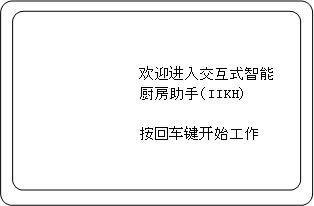
\includegraphics[scale=0.65]{rdd-example.png}
\caption{IIKH}
\label{fig:iikh}
\end{figure}


简单地讲,交互式智能厨房助手(the Interactive Intelligent Kitchen Helper,IIKH)是一个基于PC的应用程序,它将取代在通常厨房中所使用的食谱索引卡系统。除了维护食谱数据库之外,IIKH还可以帮助确定一段时间内的饮食计划——比如一个星期内的计划。IIKH的使用者可以通过软件的终端浏览食谱数据库,以交互的方式创建一系列新菜谱。IIKH会自动针对原料的种类和数量来调整食谱。为某一周、某一天或者是某一餐打印出菜谱清单,而且还能打印出一段时间内的食谱所需要的所有原料的详细清单。


事实上,大多数软件系统的最初描述和IIKH一样,在初始阶段,系统规范在很多关键点上的描述都非常模糊。

另外一个事实是,无论如何,软件系统的最终设计和开发要靠多人的协同合作,因此设计小组的初始目标是必须澄清描述中的模糊之处,将项目合理地划分成多个组件并分配给每个小组成员进行开发。

面向对象编程的基石是将软件通过行为(action,即将要执行的动作)使之特性化,将在每个系统的各个级别的开发上都得以体现。

最初,小组会通过很高级别的抽象手法来特性化整个应用程序的行为。由此产生了不同的软件子系统的行为描述。只有当所有的行为都被确定和描述之后,软件设计小组才能进入编码(coding)阶段。

强调行为是面向对象编程的一个标志,在系统的最初描述中就可以确定行为,远远早于能够确定其他设计观点的时刻。

由于不断地被行为所驱动,因此从问题描述开始,通过软件架构、代码开发直到应用程序完成,责任驱动设计可以实现这个过程的平稳过渡。

\section{Scene}


第一个任务就是细化软件规范。最初的规范,除了一些最宏观的概念外,总是存在大量的模棱两可和不确切的方面。这一步就几个目标,其中一个目标就是能够对最终产品的表象(外观和感觉)进行更好的控制。

这些信息可以反馈给我们的客户,然后看看他是否同意我们的构思。最终应用程序的规范在软件系统的构建过程不可避免地要经常更改,因此重要的是软件的设计要能够适应变化,并且尽早地注意潜在的变化。

同样重要的是,现在所做出的非常高级别的决策抽象会影响到最终软件系统的结构,而且特别要注意的是,我们在设计中将要执行的活动会体现出各个组件的内部结构。

为了揭示系统的基本行为,我们的设计小组首先建立了一系列场景,即将应用程序的运行情况通过场景来模拟表示,就像已经拥有了一个正常工作的系统一样。



一个复杂的物理系统工程,可以通过将其分解成更小的单元而简化设计。同样,软件工程也可以通过标识和开发软件组件来简化软件系统设计。

组件仅仅是抽象的实体,它可以执行一定的任务(即完成一定的责任)。从这方面来讲,没有必要精确地了解组件的详细描述,也没有必要了解组件执行任务的细节。

一个组件最终可以转变成一个函数、一个结构、一个类或者是其他组件的集合。在这个开发层次上,组件有以下两个重要的特性:

\begin{compactitem}
\item 组件必须拥有一套小的且定义明确的责任集合;
\item 组件应该尽可能地减少与其他组件的交互;
\end{compactitem}


当设计小组遍历完他们所设计的所有场景之后,便开始对将要执行某项任务的组件进行标识。每一项必然发生的活动都要被标识,并且作为责任分配给某一组件,如下图所示。


\begin{table}[htbp]
\centering
\begin{tabular}{|l|l|}
\hline
组件名称 & 协作组件\\
\hline
分配给该组件的责任描述&其他组件列表\\
\hline
\end{tabular}
\end{table}

在软件需求分析过程中,可以用小型索引卡来表示组件,索引卡上写明软件组件的名称、组件的责任以及必须与该组件交互的其他组件。

CRC卡是由Beck发明的,CRC代表了Component、Responsibility和Collaborator,即组件、责任和协作组件,CRC卡与每一个相应的软件组件关联,上面记录了该组件的责任。

通过场景工作时,有必要将CRC卡分配给设计小组的不同成员,持有代表组件的CRC卡片的成员需要记录与卡片相关联的软件组件的责任,并且在场景模拟期间担任软件“代理人”的角色。当软件系统需要另外一个组件的服务时,他(或她)描述软件系统的活动,将“控制”传送给其他成员。

使用CRC卡可以对各种不同的软件设计方案进行试验、研究或弃用。

卡片的物理分离可以加深设计人员对不同组件之间的逻辑分离的重要性的理解,而组件之间的逻辑分离可以强化内聚性和耦合性,同时CRC卡的版面限制也是估量软件系统的复杂程度的量度。

如果一个组件的CRC卡所提供的版面无法容纳这个组件需要执行的任务,那么这个组件可能是过于复杂了,这个时候设计小组应该寻找更加简单的解决方案,实际应用中可以通过将部分责任转移到其他组件,从而将一项任务分配给两个或者更多的新组件。


在小组讨论时,组件的标识发生在对工作系统的执行情况进行构想的过程中,这个过程的进行通常是通过循环来回答“什么/谁”这个问题。

首先,设计小组确定下一步执行什么活动,紧接着就要回答谁来执行这项活动这个问题。以这种方式设计一个软件系统,与组织一群人(例如俱乐部)很相似。


任何将要执行的活动都必须以责任的形式赋予给某个组件。只有分配一个主体去执行一项行为,这项行为才能发生。这也如同一个俱乐部的运行,任何活动的执行都必须分配给某些个人,在组织一个面向对象系统编程的过程中,所有的活动都必须分配给某些组件来负责。优秀的面向对象设计的秘诀就是先对每项活动建立一个主体。

\section{Document}

从场景分析阶段开始,就应该认识到,有两份文档应该是任何软件系统的基本组成部分:用户手册和系统设计文档,这两项工作需要在编码之前开始。

用户手册从用户的角度描述了用户与系统之间的相互作用,这是一种验证开发小组对应用程序的理解与用户对应用程序的理解是否一致的有效手段。在创建场景中所作的决定应该密切符合用户对最终应用程序要求,因此用户手册的开发要紧跟场景开发的进程。

在任何实际代码开始编写之前,软件设计小组对应用程序的理解与最终用户十分接近。这样软件开发者才能够很容易地理解那些对于初学者用户需要解决的问题。

用户手册同时也是一个优秀的工具,它可以验证开发小组看待问题的方式与客户是否相同。客户很少能够给开发小组提供一份详细而正式的规范,因此,客户和开发小组之间需要进一步确认的问题和相互的交流应该在正式编程开始之前就尽早进行,这样可以防止以后出现大的分歧。

第二个基本文档是设计文档,设计文档记录了软件设计中的主要决定,这些决定应该在设计者对各项要求都思路清晰的情况下产生,而不是在许多相关细节都快忘记之后才进行设计。在开发阶段早期,通常很容易书写软件系统的全局描述。但是很快,开发工作的重心会转移到每个组件或者模块的级别上。尽管进行模块级文档设计也是很重要的事情,但是,如果设计文档过多地关心每个模块的细节,将使以后的软件维护人员很难对软件系统的整体结构形成一个概要的了解。

CRC卡是设计文档的一个方面,但是许多其他重要的决定并没有通过它反映出来。任何关于主要设计的支持或反对的讨论,以及影响最终决定的因素都应该记录下来。应该维护项目进度的日志和日记,而且在整个开发过程中,用户手册和设计文档也要随着软件的不断改进而即时地改进,保持与软件同步。

\section{Action}


在场景设计阶段,开发小组决定在系统开始时,呈现在用户面前的是一个吸引人的信息丰富的窗口。我们将展示这个窗口的责任分配给一个叫做Greeter(问候者)的组件来完成。

通过某种还未确定的方式(可能是下来菜单、按钮、按键或者显示屏),用户可以从几项活动中选择一项。最初,开发小组只确定了五项活动:

\begin{compactitem}
\item 自由浏览现存食谱的数据库,但是不涉及任何特定的就餐计划;
\item 对数据库增加新食谱;
\item 编辑或注解一个已有食谱;
\item 检查已存在的食谱计划;
\item 建立一个新的食谱计划;
\end{compactitem}

这些活动可以分成两组:前三条与食谱数据库有关,后两条与饮食计划有关,因此开发小组下一步决定创建与这两项责任对应的组件。

继续场景,开发小组选择暂时忽略就餐计划管理,先着手细化Recipe Database(食谱数据库)组件的活动。例如,下面显示了用来表示“问候者”组件的最初的CRC卡。

\begin{table}[htbp]
\centering
\begin{tabular}{|l|l|}
\hline
问候者			&协作组件\\
\hline
显示丰富的初始化信息&	数据库管理者\\
\hline
为用户提供活动选择&	计划管理者\\
\hline
食谱数据库管理者 & \\
\hline
计划管理者 & \\
\hline
\end{tabular}
\end{table}



泛泛地讲,食谱数据库组件的责任就是维护食谱集合。现在,已经可以确定这项任务的三个要素:食谱数据库组件必须便于浏览现有的食谱库、编辑食谱以及增加新食谱到数据库。


有很多关于如何让用户更好地浏览数据库的问题必须到最后才能决定。比如,最初是否应该展现给用户食谱分类清单(如汤、沙拉、主食和甜点等)?用户在输入关键字进行限定搜索时,是通过提供配料清单选择当前关键词,查看所有包括这些配料(例如杏仁、草莓和奶酪)的食谱,还是通过提供以前的搜索关键词(例如Bob最喜欢的蛋糕名称)来选择当前关键词进行搜索?

思考上面这些问题会很有意思,但是最重要的地方却是不需要在此时对这些问题做出决定。因为它们只影响一个单独的组件而不影响系统其他功能,继续场景时应该忽略这些,假定用户通过某种方式已经选中一个特定的食谱。


永恒不变的就是偶然与变化的必然性,在软件开发中也是如此。无论我们怎样认真仔细地进行软件系统的设计,几乎可以确定的是,在系统开发的某一时刻,用户的需求会发生改变,并强求软件做出相应的变化。软件开发人员和软件设计人员都需要预测这些变化,并且做出相应的变化。


\begin{compactitem}
\item 基本原则是变化影响尽可能少的组件,即使是应用程序的外观或者功能发生大的改变,也应尽量只改变代码的一至两个部分。
\item 尽量预测可能发生变化的源头,并通过尽可能少的软件组件将这种变化的影响隔离开来。最可能发生变化的来源有界面、通信方式和输出格式等。
\item 尽量隔离或减少软件对硬件的依赖。例如,应用程序中的食谱浏览界面可能部分依赖于系统运行的硬件平台,但是未来软件发布时可能需要移植到不同的平台。一个良好的设计应该预测到这些变化。
减少软件组件之间的耦合性会降低组件之间的依赖性,当其中一个组件发生变化时,与之相关的组件能够尽可能地减少影响。
\item 设计文档应该详细记录所有主要决定的设计过程和讨论记录。与发布最初软件版本时相比较,在发布未来软件版本时,几乎可以肯定地是,软件维护人员或设计人员将发生部分变动。设计文档应该使未来的每一个小组成员都了解每一项决定背后的重要因素,帮助他们避免花费时间来讨论一些已经解决过的细节。
\end{compactitem}

每一个食谱都与一个特定的食谱组件相关联,一旦选定一个食谱,控制信息就会传送到相关的食谱对象。

一个食谱必须包含确定的信息,基本上包括配料清单和将配料做成最后食品的操作步骤。在我们的场景中,食谱组件还需执行其他活动。例如,它将以交互的方式在屏幕上显示食谱,并且用户可以被授权注解或改变配料清单和操作步骤,用户还可以选择是否打印食谱。所有这些行为都是Recipe(食谱)组件的责任。

现在,我们将继续讨论独立形式的“食谱”组件。在设计的过程中,可以把它看作是代表许多实际食谱的原型食谱,以后我们将继续进行独立组件和多重组件的对比讨论。

通过上面的分析可以知道,允许用户浏览数据库是一项必然发生的行为。

现在,我们将开始分析数据库管理组件,假定用户希望新增一个新的食谱,数据库管理组件以某种方式将新食谱加入某一类别中,要求用户录入新食谱的名称,然后创建一个新食谱组件,显示供用户编辑的空白输入框。因此,执行这项新任务的责任是允许用户编辑已有食谱的责任集合中的一个子集。

分析完浏览和创建新食谱后,下面将分析“问候者”组件,研究每日食谱计划的开发,这是Plan Manager(计划管理者)组件的任务。

用户能够以某种方式保存已有计划,因此用户即可以从检索一个已创建的计划开始,也可以从创建一个新计划开始。在后一种情况下,用户将面对一些计划的日期,每一个日期都与一个独立的Date(日期)组件相关。

用户可以选择一个特定的日期来进一步查看,这时控制就会传送到相应的“日期”组件。“计划管理者”的另外一项活动就是打印出计划期间的食谱。最后,用户可以指示“计划管理者”组件列出这些食谱所需的全部杂货。

“日期”组件需要维护每一餐的集合以及用户提供的备注信息(生日聚会、周年庆典、纪念宴会等)。日期组件还要打印关于指定日期的信息。通过某种方式,用户可以要求“日期”将关于指定日期的所有信息打印出来,或者选择进一步查看就餐细节。在后一种情况下,控制将传送给Meal(膳食)组件。

\begin{compactitem}
\item “膳食”组件维护扩展食谱集合,这里“扩展”是指用户增加一倍、两倍或者一个食谱。
\item “膳食”组件显示关于一餐所用的全部食物信息。用户可以从中添加、删除任何食谱,也可以将信息打印出来。
\end{compactitem}

为了发现新的食谱,必须让用户能够浏览食谱数据库。因此,“膳食”组件就必须与食谱数据库组件交互。设计小组以这种形式继续研究各种可能的场景。

到现在为止,我们还没有设计开发的场景主要就是关于如何处理例外情况。例如,一个用户选择搜集一个食谱的关键词,却没有与之相匹配的食谱,这时系统就需要确定该如何将这种信息反馈给用户。还有就是如果一个用户取消某个搜索行为,例如,用户输入一个食谱名称开始搜索之后,却又放弃了该搜索。每一种情形都应该考虑进去,处理不同情况的责任要分配给一个或更多的组件去执行。

设计完成各种场景之后,软件设计小组最后决定将所有的活动适当地分配给6个组件来完成,其中:

\begin{compactitem}
\item “问候者”组件只需与“计划管理者”组件和“食谱数据库”组件进行通信。
\item “计划管理者”组件只需与“日期”组件通信,“日期”组件只需与“膳食”组件进行通信。
\item “膳食”组件与“食谱管理者”组件进行通信,并且通过这个代理,与特定的食谱进行通信。
\end{compactitem}

\begin{figure}[htbp]
\centering
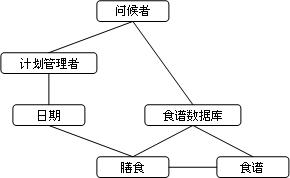
\includegraphics[scale=0.65]{rdd-example-component.png}
%\caption{}
%\label{rdd-example-component}
\end{figure}

对于难以定义的问题,基于行为的设计技术要比基于数据结构的设计技术更易于使用。

\section{Diagram}

在表明组件之间的静态关系后,不过仍然不适合描述在场景执行过程中组件之间的动态关系,描述组件之间动态关系的更好的工具就是交互图表。下图显示了交互式智能厨房助手的交互图表的开始情况。



\begin{figure}[htbp]
\centering
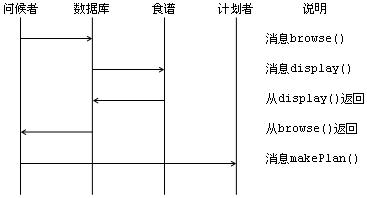
\includegraphics[scale=0.65]{rdd-example-diagram.png}
%\caption{}
%\label{rdd-example-diagram}
\end{figure}


在图表中,从上到下表示时间从后到前。每个组件由一条垂直线来表示。用从一条垂直线指向另一条垂直线的水平箭头线来表示一个组件将一条消息传递到另外一个组件。类似地,组件返回的控制或返回调用者的结果值也用箭头线来表示(有时候也用两种不同的箭头形式来表示,比如用实线表示消息传递,虚线表示返回控制)。图表右侧的说明更加详细地解释了正在进行的交互。

通过时间轴,交互图表可以更加清晰地描述场景中事件的顺序。因此,交互图表是用于复杂软件系统的有效文档工具。


\section{Component}


\section{Action \& State}



组件通过行为,即通过它能够做什么来表现它的特征,但是同时组件也可以包含确定的信息。把IIKH中的一个“食谱”结构作为原型组件,查看这样的组件的一种方式就是把它看作是一个由行为和状态组成的对象。


\begin{compactitem}
\item 组件的行为是指组件所能执行的一系列动作。对一个组件所有行为的完整描述有时称为协议。对于“食谱”组件来说,协议所包含的行为有编辑准备命令、在终端屏幕上显示食谱或打印食谱等。

\item 组件的状态是指某一特定时刻组件所包含的所有信息。对于“食谱”组件来说,状态包括配料和准备指令。
\end{compactitem}

状态不是恒定的,而是可以随时间变化的。例如,用户通过编辑一个食谱(行为),可以改变准备指令(部分的状态)。

不是所有的组件都必须维护状态信息。例如,可能有这样的情况,由于“问候者”组件不需要在执行过程中记录任何信息,因此它可以没有任何状态信息。然而,大部分组件都是由行为和状态结合而成的。

\section{Instance \& Class}


状态和行为的分离使我们澄清了在以前的讨论中所避开的观点。需要注意的是,在实际的应用程序中可能会有很多不同的食谱。然而,所有这些食谱都会以同样的方式执行其行为,也就是说,每个食谱的行为都是相同的,只有状态——各种配料清单和准备命令——对于不同的食谱是不一样的。在开发的早期,我们的注意力应集中在所有食谱的共同行为特征上,每一个食谱的特定细节并不重要。

\begin{quote}
\textsl{类用来描述一系列有相似行为的对象。}
\end{quote}

在几乎所有的面向对象语言中,类还用于语法结构,类的具体表现个体称为实例。

行为是和类相联系,而不是和个体相联系。也就是说,一个类的所有实例都以相似的行为来响应同一命令。

另一方面,状态是个体的特性,我们可以在“食谱”类的各个实例中看到这一点,它们都能执行相同的动作(编辑、显示、打印),但是,使用的数据却是不同的。

\section{Coupling \& Cohesion}



软件组件设计中的两个重要概念就是耦合性和内聚性。

\begin{compactitem}
\item 内聚性就是一个独立组件的所有责任组成一个有意义的单元的聚合程度。
\item 耦合性描述了软件组件之间的关系。
\end{compactitem}

通过某种方式将一个独立组件的任务联系起来可以使一个组件获得较高的内聚性。可能最常用的联系任务的方式就是通过观察,将存取公共数据值的一组任务放在一起。例如,“食谱”组件的各种责任就是这项原则的一个应用。


一般情况下,由于软件组件之间的联系阻碍了软件的开发、修改或复用的简易性,因此应尽可能地减少耦合的数量。

特别是,当一个软件组件必须访问的数据值(状态)由另外一个软件组件控制时,耦合数量就会增加,应该尽量避免出现这种情况,这将有利于把任务转移到包含必需数据的组件的责任列表中。例如,由于当“食谱数据库”组件执行相关行为时,需要首先编辑食谱,因此设计人员可能会自然地把编辑食谱的责任先指定给“食谱数据库”组件。但是,如果我们这么做,“食谱数据库”代理就需要有直接操作每一个食谱状态(表示配料清单和准备指令的内部数据值)的能力,把编辑食谱的责任转移给“食谱”组件是避免这种紧密联系的一种更好的设计。

\section{Interface \& Implement}


通过行为将一个软件组件特征化,有一个非常重要的结果。一个程序员可能知道如何使用由另外一个程序员开发的组件,但却不需要知道组件是如何实现的。例如,假定把IIKH中的六个组件分配给不同的程序员来开发,开发“膳食”组件的程序员应该允许IIKH用户浏览食谱数据库,并且对某一餐选定一份食谱。要达到这个目标,“膳食”组件只需调用与“食谱数据库”组件相关的“浏览”行为即可,“浏览”行为被定义成返回某一个食谱。这个过程不需要了解“食谱数据库”组件使用的具体实现方式,就可以执行实际的浏览行为。


这种有目的地忽略一个简单接口后面的实现细节的行为称为信息隐藏。我们说,组件封装了行为,它只显示如何使用组件而不显示它执行的细节行为。这自然而然地导致了关于软件系统的两种不同的视角。接口的视角就是指能够被其他程序员看到的界面,它描述了一个软件组件能够执行什么。实现的视角就是指能够被开发特定组件的程序员看到的界面,它描述了一个组件如何完成一项具体任务。


接口与实现的分离可能是软件工程中最重要的概念,然而这对于大多数新手来说仍然是很难理解的。信息隐藏只有在多人合作编程的项目背景下才非常有意义。对于这种工作,限制因素通常不是项目包含代码量的多少,而是程序员之间以及他们各自的软件系统之间的相互交流是否充分。软件组件通常是由各个相互独立的程序员并行地进行开发的。

对于项目开发来说,通用软件组件的复用性变得越来越重要。如果组件成功地复用到系统中,则系统不同部分之间的连接将会减少且容易理解。David Parnas用以下两条原则(称为Parnas原则)来描述这些观点:

\begin{compactitem}
\item 软件组件的开发者必须向目标用户提供所有能用来有效使用组件所提供的服务的信息,而无需提供其他任何信息。
\item 必须向软件组件的开发者提供所有需要用来执行分配给组件的责任的信息,而无需提供其他信息。
\end{compactitem}

接口从实现中分离的结果是,程序员可以在不影响其他软件组件的条件下,对多个具有同一结构、不同实现的组件进行试验。


\section{Formal Interface}

在继续细化组件的开发的过程中,接下来的第一步就是对通信模式和通道进行形式化。应该制订适合于实现每个组件的关于总体结构的设计原则。对于只有一种行为且没有内部状态的组件,可以把它做成一个函数——例如,一个组件只是处理一个字符串,把所有大写字母改成小写字母。

对于执行多项任务的组件,可能更容易用类来实现。对每个组件CRC卡上所标识的责任进行命名,这些名称最终会映射成方法名。与方法名一起,所有传给函数的参数类型也要标识。下一步,还应该描述组件本身的信息,并且对所有的信息都要进行解释说明。如果一个组件需要某些数据项执行一项特定的任务,数据来源(可以通过参数、全局变量值,也可以通过由组件内部维护的局部变量值)一定要明确地标识。

应该仔细思考如何对不同的行为进行命名。Shakespeare曾经说过,一个名称的变化不会改变所描述的对象,但是对于聆听者来说,不是所有的名称都能在头脑中产生相同的想象。

\begin{compactitem}
\item 名称创造了词汇,通过词汇形成最终的设计,因此选择一个有意义的名称是非常重要的。
\item 名称应内部一致、有意义、尽量简短,还要能够让人联想到问题的背景。
\end{compactitem}

通常要花大量的时间去寻找恰当的术语来描述将要执行的任务和操作的对象,而且在设计前期,恰如其分地命名绝对不是一件毫无意义的事情,它可以极大地简化和促进以后的工作。

建议命名时遵循以下基本原则:

\begin{compactitem}
\item 使用可发音的名称,根据经验,如果名称不能被大声地读出来的话,它就不是一个好名字。
\item 用大写字母(或下划线)标出名称中新词的开始,例如命名成“CardReader”或“Card\_reader”,而不是难以辨认的“cardreader”。
\item 仔细检查缩略语,一个对某人来说非常清楚的缩略语,对另外一个人可能比较费解。例如,“TermProcess”是指一个结束的进程还是一个与终端相关的进程呢?
\item 避免有多种解释的名称。“empty”函数是说明一个对象为空,还是清空一个对象的值?
\item 名称中避免使用数字。数字在某些情况下很容易被读成字母(例如“0”与“o”,“1”与“l”,“2”与“z”,“5”与“s”等)。
\item 函数和变量的名称表示布尔值时,可以清楚地表达“真”值或者“假”值,例如“PrinterIsReady”清楚地表明“真”值代表打印机正常工作,但是如果使用“PrinterStatus”无法做到精确。
\item 对于那些代价大且很少发生的操作的命名,要格外注意。这样才可以避免由于错误的函数而引起的错误。
\end{compactitem}


一旦为每一个行为选好名称,就要重新改写每一个组件的CRC卡,写上代表每个确定行为的函数的名称和形参。下图是一个关于“日期”组件CRC卡的例子,只是现在仍未确定的是,每个组件如何执行相关的任务。


\begin{table}[htbp]
\centering
\begin{tabular}{|l|l|}
\hline
日期							&协作组件\\
\hline
							&计划管理者\\
\hline
维护制定日期的信息			&膳食\\
\hline
Date(year,month,day)	——建立一个新日期&\\
\hline
DisplayAndEdit()		——在窗口显示用户可以编辑的日期信息&\\
\hline
BuildGroceryList(List\&)	——把所有膳食的原料增加到杂货列表&\\
\hline
\end{tabular}
\end{table}



确定场景或者角色的模拟应该在更详细的层次上进行,以保证所有活动得以分配,也保证所有必需的信息得以维护且能够被责任组件利用。

在设计表现时,不同于以往,设计团队可以分为几个小组,每一小组负责一个或多个软件组件,任务是将组件描述转化成软件系统的实施。这一过程的主要工作是设计数据结构,每个子系统通过这些数据结构来维护状态信息,进而完成所分配的责任。

数据结构的选择是软件设计过程的核心。一旦选定了数据结构,在完成责任时,组件所使用的代码通常就可以清晰了。但是数据结构一定要与当前的任务相匹配。错误的选择将导致程序复杂而低效,而正确的选择却能达到完全相反的效果。

还应注意,行为的描述也必须转换成算法。这些描述应与协作组件即将执行的任务相匹配,以保证这些任务得以实现,并提供执行每个过程时所需的必要数据。


完成每个软件子系统的设计后,下一步就是实现组件的期望行为。如果前面的步骤执行正确,每一项责任或行为就可以用简要的描述来表示。这一步的任务就是用计算机语言实现所期望的活动。如果没有被早些确定(指作为系统规范的一部分),那么现在可以做出决定的问题都处在一个单独组件的内部。

随着多人协作编程项目变得越来越普遍,由一个程序员来完成一个系统的所有方面的现象变得越来越少。通常,程序员需要掌握的技能就是知道代码的某一部分如何融入整体框架,以及和团队的其他成员如何协同工作。

一般情况下,在组件的实现过程中,将哪些特定信息和行为分配给哪些“隐藏在幕后”的其他组件是很清楚的,从用户的角度来说,软件抽象极少或者没有,因此有时会称这样的组件为facilitators。

将软件子系统逐个实现和测试完成之后,就可以对它们进行集成,形成最终的产品。

组件集成并不是孤立的一个步骤,而是一个过程的某一部分。从一个简单的基础系统开始,逐渐地将各个子系统增加到这个系统中并且使用存根(stub)——没有行为或只有有限行为的简单虚构的例程——对这个还没有生效的部分做测试。

例如,在IIKH的开发过程中,从“问候者”组件开始集成是非常合理的。为了单独测试“问候者”组件,就要为“食谱数据库管理者”组件和日常的“膳食计划管理者”组件编写存根。这些存根的工作仅仅是显示必要的消息和返回。通过这些存根,组件开发小组可以测试“问候者”系统的各个方面(例如,对按键做出正确的响应)。测试独立的组件通常称为单元测试。

紧接着,可以用更加完整的代码来替代一个或更多的存根。例如,开发小组可能决定用实际的系统来代替关于“食谱数据库”组件的存根,同时保持其他部分的存根不动。然后,进一步的测试继续进行,直到系统完全按照所期望的情况来工作(这通常称为集成测试)。
	

当所有的存根都被工作组件代替后,应用软件才最终完成。有意识地减少组件之间联系的设计目标,极大地方便了独立组件的测试,因为这降低了对大规模存根的需要。

在集成过程中经常会出现这样的情况,在某一软件系统中出现的一个错误,却是由另外一个系统中的代码错误所导致的。因此,集成测试将会发现错误,而这又导致某些组件的更改。变更组件后,在进行软件的再次集成(进而,是系统的再次集成)以前,组件应该重新独立测试。当一个组件变更后,这时就需要重新运行以前的测试用例,称为回归测试。


认为应用程序的工作版本一旦交付,软件开发小组的任务就已完成的想法的确很吸引人。但是不幸地是,这几乎从未实现过。软件维护是指软件系统的初始工作版本交付之后的后续工作。属于这个范畴的工作各种各样,主要包括以下几个方面:


\begin{compactitem}
\item 在交付后的产品中还会发现错误或者bug。通过对现有版本或者后续版本进行更正来解决这些问题。
\item 需求可能变化,可能是由于政府法规,也可能是由于产品标准。
\item 硬件可能改变。例如系统可能移植到不同的平台,或者使用不同的输入设备(如手写笔或触摸屏等),此时要求系统能够正常使用。输出技术也可能变化,例如,从基于文本的系统迁移到基于图形的视窗系统。
\item 用户期望可能变化,用户可能要求更强大的功能、更低的费用和/或更容易使用,这些可能是同类产品竞争的结果。
\item 用户可能会要求更好的文档
\end{compactitem}

优秀的设计应该认识到变化的不可避免性,并且从一开始就制定出与这些变化相适应的计划。


















\part{Class}

\chapter{Introduction}




\section{Overview}

最简单地来说,类就是定义了一个新的类型和一个新的作用域。


\subsection{Data Structure}


类(class)是一种面向对象计算机编程语言的构造,描述了所创建的对象共同的属性和方法,用户可以使用C++中的类来定义自己的数据结构。

\subsection{Class Type}


事实上,C++设计的主要焦点就是使用类和操作符重载等来实现用户定义的类类型(class type)的行为与内置类型的一致性。例如,C++中的istream和ostream等库类型都是定义为类的,严格来说它们都不是语言本身的一部分。


类有接口和结构,而且可以将实现和接口分离。



\begin{compactitem}
\item \textsl{接口描述了如何通过方法与类及其实例互操作;}
\item \textsl{结构描述了一个实例中数据如何划分为多个属性。}
\end{compactitem}

类类型通常被称为抽象数据类型,其数据(即状态)和作用于状态的操作将被视为一个单元,因此抽象数据类型构成了面向对象编程和泛型编程的基础。



\subsection{Class Member}


类是创建对象的蓝图,其更严格的定义是由某种特定的元数据所组成的内聚的包。


类定义了数据成员和函数成员,其中:

\begin{compactitem}
\item 数据成员用于存储与类类型的对象相关联的状态,应该仅在类的私有部分定义数据成员;
\item 函数成员负责执行赋予数据意义的操作。
\end{compactitem}

类可以没有成员,也可以定义多个成员,成员可以是数据、函数或类型别名等,所有成员必须在类的内部声明。


另外,类提供了一种特殊的成员函数——转换函数来定义类类型对象之间的隐式转换,从而使编译器可以对对象实现与内置类型一致的转换。



除了定义数据和函数成员之外,类还可以定义自己的局部类型名字(或类型别名),最后以分号\footnote{按照C语言的传统,在类的定义之后接一个对象定义列表,因此类定义必须以分号结束。}结束类的定义。

\begin{lstlisting}[language=C++]
class Screen{
public:
	// interface member functions
	typedef std::string::size_type index;
private:
	std::string contents;
	index cursor;
	index height, width;
};
\end{lstlisting}

重载的成员函数和普通函数应用相同的规则:两个重载成员的形参数量和类型不能完全相同,调用非成员重载函数所用到的函数匹配过程也应用于重载成员函数的调用。

\begin{compactitem}
\item 成员函数可以被重载,但是只能重载所在类的其他成员函数。
\item 成员函数与普通的非成员函数以及在其他类中声明的函数不相关,也不能重载它们。
\end{compactitem}

\subsection{Instance}

用户在定义类实际上就是定义了一个类型,然后就可以和使用内置类型一样定义指定类型的对象。


\begin{compactitem}
\item 在类型定义阶段,编译器不进行存储分配;
\item 在对象定义阶段,编译器就会为对象分配存储空间。
\end{compactitem}


\begin{lstlisting}[language=C++]
class Screen{
public:
	// interface member functions
	typedef std::string::size_type index;
private:
	std::string contents;
	index cursor;
	index height, width;
};

Screen item;
\end{lstlisting}


一般来说,类描述了一些对象的行为规则,而这些对象就被称为该类的实例(instance),通常只有由类定义的操作可被用于对象。


\begin{compactitem}
\item 类是与某个层的对象的最具体的类型,而且类还可以有运行时表示形式(元对象),这样就可以为操作与类相关的元数据提供运行时支持。
\item 对象代表实际的存储空间,而且每个对象具有自己的类数据成员的副本。
\end{compactitem}



用户使用类来定义自己的抽象数据类型时,数据抽象能够隐藏对象的内部表示,同时仍然允许执行对象的公有(public)操作。


大多数支持类的编程语言都支持不同形式的类继承,而且许多语言还支持提供封装性的特性(比如访问修饰符)。

类为面向对象编程的三个最重要的特性(封装性、继承性和多态性)提供了实现的手段,类背后蕴藏的基本思想就是数据抽象和封装。

\begin{compactitem}
\item 数据抽象依赖于接口和实现的分离。
\item 封装将低层次的元素组合起来形成新的、高层次的的实体。
\end{compactitem}

例如,函数就是封装的一种形式,其所执行的细节行为被封装在函数中,从而可以调用一个函数,但是不能访问其所执行的语句。

封装层次更高的类也是一个封装的实体,其代表了若干成员的聚集,大多数(设计良好的)类类型都隐藏了实现该类型的成员。

例如,标准库类型vector等同时具备数据抽象和封装的特性。数组在概念上类似于vector,但是既不是抽象的,也不是封装的,用户可以通过访问存放数组的内存来直接操作数据。

并非所有类型都必须是抽象的,具体类会暴露而非隐藏其实现细节。例如标准库中的pair类就是一个实用的、设计良好的具体类(而不是抽象类),pair类型只是将两个数据成员捆绑成单个对象。


自行车制造商一遍一遍地重用相同的蓝图来制造大量的自行车,开发人员可以使用相同的类(即相同的代码)来一遍一遍地建立对象。



\section{Abstraction}


在现实世界中,经常有属于同一个类的对象,例如某辆自行车只是世界上很多自行车中的一辆。同样地,在面向对象软件中,也有很多共享相同特征的不同的对象—矩形、雇用记录和视频剪辑等,可以利用这些对象的相同特征为它们建立一个蓝图。

对象的软件蓝图就是类,通过类可以定义所有一类对象的变量和方法的蓝图或原型。例如,可以建立一个定义包含当前档位等实例变量的自行车类,这个类也定义和提供了实例方法(变档、刹车)的实现。

\begin{compactitem}
\item 类不是它描述的对象,例如自行车的蓝图不是自行车,对象则是现实世界的电子模型或抽象概念。
\item 抽象类被定义为永远不会也不能被实例化为具体的对象。
\end{compactitem}

实际上,抽象类往往用于定义一种抽象上的概念,在类的继承关系中它往往被定义在较上层的位置。

抽象类与接口存在类似的地方,二者都偏重于对共通的方法和属性进行规约,但是抽象类往往可以规约一个共同的方法和属性时提供一个对他们的实现。

以现实世界为例,"水果"可以算作一个抽象类,"苹果"和"香蕉"则可以作为它的派生类,它们的区别在于"水果"是个概念,它不会有实例,但是"苹果"和"香蕉"则肯定会有实例。

实例变量的值由类的每个实例提供。例如,当创建自行车类以后,必须在使用之前对它进行实例化。



当创建类的实例时,就建立了这种类型的一个对象,然后系统为类定义的实例变量分配内存,这样就可以调用对象的实例方法来实现一些功能。

相同类的实例共享相同的实例方法。除了实例变量和方法,类也可以定义类变量和类方法。

操作系统在第一次在程序中遇到一个类时为这个类建立它的所有类变量的拷贝 - 这个类的所有实例共享它的类变量。


从类的实例中或者从类中都可以访问类变量和方法。类方法只能操作类变量,不必访问实例变量或实例方法。



\section{Encapsulation}

所有的面向对象编程语言都共有这些相同的概念:类、实例、消息传递、方法和继承等。


用户可以从多个角度考虑面向对象编程(尤其是对象),因此在不同的面向对象编程语言中,使用不同的术语来表示相似概念是很普遍的事情。

在面向对象设计中引入了不同的抽象层次,通过这些层次来检查程序,这样从高级抽象的角度可以将对象看作是抽象数据类型的实例。

数据抽象是一种有效的解决问题的方式,它将某些信息有意识地隐藏在程序的某个部分。例如,用户开发的一系列抽象数据类型都可以从两个方面来看待。

与Parnas原则相似,从外部来看,抽象数据类型的客户(用户)只能看到抽象行为的操作集合,作为抽象数据类型的另一接口,定义抽象的实现者通过数据变量可以来维护对象的内部状态。

例如,对于堆栈(Stack)的抽象,用户只能看到合法操作的描述—如push、pop和top。另一方面,实现者需要了解用来实现抽象的具体数据结构,这样具体的细节就被封装在更加抽象的框架中。

\begin{figure}[htbp]
\centering
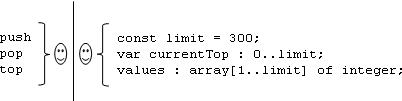
\includegraphics[scale=0.6]{stack.png}
\caption{堆栈的接口和实现}
\label{fig:stack}
\end{figure}

一般使用实例(instance)来表示类的一个具体代表或范例。相应地,使用实例变量(instance variable)来表示实例所维护的内部变量,有时也会使用数据字段(data field)或数据成员(data members)来表示这一概念。

每个实例都有它自己的实例变量集合,客户不能直接改变这些值,只有和类相关的方法才能改变它们。

对象可以简单地看作状态(state)和行为(behavior)的结合,其中状态由实例变量来描述,而行为由方法来表示。

\begin{compactitem}
\item \textsl{从对象外部来看,客户只能看到对象的行为;}
\item \textsl{从对象内部来看,方法通过修改对象的状态以及和其他对象的相互作用来提供适当的行为。}
\end{compactitem}

\chapter{Declaration}


\section{Forward Declaration}


用户在只声明一个C++类时称为前向声明(forward declaration),结果是在程序中引入了一个不完全类型(incompete type)的类类型,这样就可以用来编写相互依赖的类。

不完全类型只能以有限方式使用,不能定义该类型的对象,因此不完全类型只能用于定义指向该类型的指针及引用,或者用于声明(而不是定义)使用该类型作为形参类型或返回类型的函数。



在创建类的对象、使用引用或指针访问类的成员之前,必须完整地实现不完全类型的类类型,这样编译器才能给类的对象预定相应的存储空间。

\begin{compactitem}
\item 只有当类定义已经定义过,数据成员才能被指定为该类类型。
\item 如果类是不完全类型,数据成员只能是指向该类类型的指针或引用。
\end{compactitem}

类不能具有自身类型的数据成员,但是可以具有指向自身类型的指针或引用的数据成员。

\begin{lstlisting}[language=C++]
class LinkScreen{
	Screen window;
	LinkScreen *next;
	LinkScreen *prev;
};
\end{lstlisting}

\section{Forward Definition}

在实践中,有时需要两个或者更多的互相引用的类,这种形式称为相互递归(mutual recursion)。例如,在表示马和马车的关系时,每一匹马需要和自己的马车联系在一起,每一辆马车又需要有一匹马。

很多语言都支持相互递归,例如Java语言在生成代码之前会扫描整个文件,这样如果程序文件的前面部分引用在文件后面声明的类,就不会产生任何冲突。

其他的语言(例如C++)会从前到后地依次处理程序文件中的类和方法,因此名称在使用之前必须至少进行部分定义。


在C++语言中必须实现向前定义(forward definition),其目的只是把这个名称置于循环中,关于定义的实现会在后面完成,这样马和马车的例子可能需要进行一定的修改。

\begin{lstlisting}[language=C++]
class Horse; // forward definition

class Buggy{
	...
	Horse * myHorse;
};

class Horse{
	...
	Buggy* myBuggy;
};
\end{lstlisting}

这里,首行仅仅表明Horse是一个类的名称,定义即将在后面出现。

对于C++编译器来说,只需知道前向定义的相关信息才能允许创建指向未知类的指针。当然,在读取类定义之前,对象不能做任何事情。

要解决这种问题,需要对类定义和与其相关的方法的实现仔细地排序:首先是第一个类的定义,然后是第二个类的定义,紧接着是第一个类的方法,最后是第二个类的方法。

\chapter{Definition}

根据语言是动态类型还是静态类型,可以把语言分为静态类型和动态类型两大类。

一般来说,静态类型语言中类型和变量有关(这种绑定通常是通过声明语句来建立的),在动态类型语言中只是把变量看作名称标识,类型和值有关。

\begin{compactitem}
\item Java、C++、C\#和Pascal语言是静态类型语言;
\item Smalltalk、CLOS和Python语言是动态语言类型;
\item Objective-C语言介于这两种类型语言之间。
\end{compactitem}

在Objective-C语言中,如果变量是静态类型,则变量可以用一个固定类型来声明。另一方面,变量也可以使用对象类型id来声明。通过这种方式声明的变量可以表示任何值,因此这种变量是动态类型。

\begin{lstlisting}[language=bash]
PlayingCard aCard;	/* a statically typed veriable */
id anotherCard;		/* a dynamically typed veriable */
\end{lstlisting}

在消息传递方面,静态类型语言和动态类型语言之间存在显著的差异。

一方面,静态类型语言在编译时使用接收器的类型来检查选择器,以确定它所接收的消息。

另一方面,动态类型语言在编译时则没有办法去核实这一消息,因此在动态类型语言中如果接收器不理解消息选择器,消息就可能产生运行时错误,静态类型语言就从来不会发生这种运行时错误。

\section{Overview}

如果通过在玩纸牌游戏来对纸牌进行抽象,可以通过一系列的细化来扩展纸牌的抽象,其中的每一次细化都会加入少量的新特征。

首先,设想将一张纸牌抽象成一个容器,那么该容器包含纸牌花色和纸牌点数这两个数据值,然后用1~13这些数字来表示纸牌的点数(1代表A纸牌,11、12、13分别代表J、Q和K纸牌)。

\begin{compactitem}
\item 如果使用的编程语言支持枚举(enum),那么可以使用枚举数据类型来表示花色。
\item 如果使用的语言不支持枚举数据类型,则可以使用符号常量和从1~4的整数值来表示花色。
\end{compactitem}


枚举数据类型的优点是可以避免类型错误,因此可以保证一张纸牌的花色一定是四种指定数值之一。如果使用整数来表示花色,就无法防止程序员把无效的整数值赋给纸牌花色变量(例如100)。



下面分别是使用不同语言(C++、Java、C\#)对类的定义的示例。

\begin{lstlisting}[language=C++]
// C++
class PlayingCard {
public:
	enum Suits { Spade, Diamond, Club, Heart };
	
	Suits suit() { return suitValue; }
	int rank() { return rankValue; }
	
private:
	Suits suitValue;
	int rankValue;
};
\end{lstlisting}

\begin{compactitem}
\item 在一个给定的C++源文件中,一个类只能被定义一次。
\item 在多个源文件中定义一个类时,每个源文件中的类定义必须是完全相同的。
\end{compactitem}





\begin{lstlisting}[language=Java]
// Java 
class PlayingCard {
	public int suit() { return suitValue; }
	public int rank() { return rankValue; }
	
	private int suitValue;
	private int rankValue;
	
	public static final int Spade = 1;
	public static final int Diamond = 2;
	public static final int Club = 3;
	public static final int Heart = 4;
}
\end{lstlisting}



\begin{lstlisting}[language={[Sharp]C}]
// C#
class PlayingCard {
enum Suits { Spade, Diamond, Club, Heart };
	public Suits suit() { return suitValue; }
	public int rank() { return rankValue; }
	
	private Suits suitValue;
	private int rankValue;
}
\end{lstlisting}


\section{Visibility}



类的可视性(visibility,又叫可访问性)修饰符用于定义抽象接口和实施封装。

\begin{compactitem}
\item C++语言的访问修饰符和冒号标明整块说明语句;
\item Java和C\#的访问修饰符分别放在每一条语句之前。
\end{compactitem}


在面向对象编程语言中都提供了一种方式用来区别以下这两种情况:一种是可以被类定义的外部(outside)了解和使用的特征,另一种是只能用于类定义内部(within)的特征。其中,后者由关键词private来表示,也就是说使用访问修饰符(public、private等)可以控制类的可视性和可操作性特征。

如果类是用struct关键字定义的,则在第一个访问修饰符之前的成员都是公有的,如果类是用class关键字定义的,则这些成员都是私有的。

\begin{compactitem}
\item 类型的数据抽象视图由其public成员定义。
\item private封装了类型的实现细节。
\end{compactitem}




在C++和C\#语言中,可以定义枚举数据类型来表示纸牌花色。其中,C++语言通过将定义语句放置在类中,可以清晰地表达这两种数据类型之间的联系。

对于C++语言,在类定义之外表示花色的常量必须以类名为前缀:

\begin{lstlisting}[language=C++]
if(aCard.suit() == PlayingCard::Diamond) ...
\end{lstlisting}

对于C\#语言,以枚举类型名为前缀:


\begin{lstlisting}[language=C++]
if(aCard.suit() == Suits.Diamond) ...
\end{lstlisting}

这里,aCard是PlayingCard(纸牌)的一个实例的名称,通过调用suit方法可以检查纸牌的花色。数据字段suitValue和rankValue表示这一抽象的实例数据。每一个PlayingCard类的实例都有自己独立的数据字段,用来维护自己的花色和点数值。

注意,花色值是通过调用suit()这一方法得到的,suit()方法只是简单地返回数据字段suitValue的数值。

大多数语言遵循的惯例是将类名的首字母大写,但并不是所有的语言都这样,尤其是C++程序中更多的是全部使用小写字母来表示类名。


一般情况下,实例变量的命名不需要首字母大写,目的是为了更容易区分类型名和实例变量名。


在Java语言还没有提供枚举数据类型\footnote{从Java 5.0开始引入了枚举类型。}时,通常的做法是定义一系列的符号常量。这里,符号常量需要使用两个修饰符final和static来修饰。

\begin{compactitem}
\item 修饰符final表示这个名称所表示的值不再改变。
\item 修饰符static的意义是不管对这个类创建多少实例,static所修饰的变量实例都只有一个。
\end{compactitem}

final和static修饰符一起作用时,就定义了一个不能改变的唯一变量—也就是常量(constant)。


在使用Java来定义类时,需要注意数据字段suitValue、rankValue和常量Spade、Diamond、Club、Heart之间的区别。其中,后者是由static来修饰的,因此它们存在于任何一个类实例的外部,并且被所有的实例共享,这类似于过程式语言中的全局变量。另外,数据字段suitValue和rankValue不是静态的,因此每个类实例都会有关于这两个数据字段的副本。

Apple公司的Object Pascal语言和Borland公司的Delphi Pascal语言(在Linux平台上称为Kylix)都是基于早期简单的Pascal语言的,因此来自原始语言的很多特征都是一样的,它们都对Pascal语言以各自的方式进行了相应的扩展。

\begin{lstlisting}[language=Pascal]
/* Object Pascal */
type 
	Suits = (Heart, Club, Diamond, Spade);
	
	PlayingCard = object
		suit : Suits;
		rank : integer;
	end;

/* Delphi Pascal */
type 
	Suits = (Heart, Club, Diamond, Spade);
	
	TPlayingCard = class(TObject)
		public 
			constructor Create(r : integer; s : Suits);
			
			function suit : Suits;
			function rank : int;

		private
			suitValue : Suits;
			rankValue : integer;
	end;
\end{lstlisting}



Object Pascal和Delphi Pascal语言都支持枚举数据类型,其中:

\begin{compactitem}
\item 前者使用关键字object来声明一个新类,因此类有时被称为对象类型(object types)。
\item 后者使用关键字class来声明新类,而且要求每一个类都必须从已有的类继承而来,这里通过继承TObject来创建新类。
\end{compactitem}

在Delphi中,类的命名惯例是以大写字母T来开头,而且Delphi语言支持访问修饰符,而Apple语言却不使用访问修饰符。另外,Delphi语言需要构造函数。


Smalltalk语言实际上不使用文本来表示类,而是使用一种称为browser的交互式界面来描述。例如,下图显示了browser的屏幕快照。

\begin{figure}[htbp]
\centering
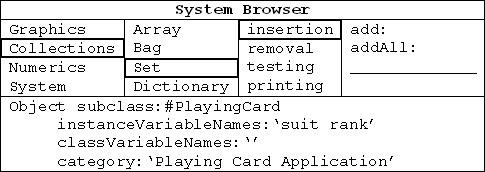
\includegraphics[scale=0.6]{smalltalk_class.jpg}
\caption{Smalltalk浏览器示意图}
\label{fig:smalltalk_class}
\end{figure}

在Browser中,用户通过将消息传递给父类Object来定义一个新类。

与Delphi Pascal语言一样,Smalltalk语言中的所有的类也必须继承于一个特定的父类。例如,上面的示意图说明了包含两个数据字段实例的PlayingCard类的创建。

下面分别是使用其他的不同语言(CLOS、Eiffel、Objective-C)对类的定义的示例。



\begin{lstlisting}[language=Lisp]
// CLOS
(defclass PlayingCard() (rank suit))
\end{lstlisting}






\begin{lstlisting}[language=Eiffel]
// Eiffel
class PlayingCard
feature 
	Spade, Diamond, Heart, Club : Integer is Unique;
	
	suit : integer;
	rank : integer;
end
\end{lstlisting}





\begin{lstlisting}[language={[Objective]C}]
enum suits { Heart, Club, Diamond, Spade };
@ interface PlayingCard : Object
{
	suits suit;
	int rank;
}
@end
\end{lstlisting}


对于类是面向对象编程最基本的概念的思想,一些语言中在其之上进行了一些改变。

Oberon语言中对于类只有比较传统的数据记录的概念。尽管如此,它还是支持消息传递以及面向对象思想中才有的对方法进行动态绑定的功能。

Oberon语言中的方法不是在记录内定义的,而是使用特殊的语法来声明方法,在参数列表中,使用一个与其他参数位置分离的参数来描述接收器。通常要求接收器是指针类型,而不是数据记录类型。

\begin{lstlisting}[language=Oberon-2]
TYPE
	PlayingCard = POINTER TO PlayingCardDesc;
		
	PlayingCardDesc = RECORD
		suit : INTEGER
		rank : INTEGER
		faceUp : BOOLEAN
	END
PROCEDUER (aCard : PlayingCard) setFaceUp (b : BOOLEAN)
BEGIN
	aCard.faceUp = b;
END
\end{lstlisting}


记录PlayingCardDesc包括数据字段,可以通过过程setFaceUp来修改数据字段,而过程setFaceUp作为接收器,必须得到关于纸牌的指针。

\section{Context}


成员函数有一个附加的隐含实参(this指针\footnote{C++类的成员函数具有一个附加的隐含形参,即指向类对象的一个this指针,与调用成员函数的对象绑定在一起。})来将函数绑定到调用函数的对象。

\begin{compactitem}
\item 成员函数不能定义this形参,只能由编译器隐含地定义。
\item 成员函数的函数体可以显式使用this指针。
\end{compactitem}

如果对类成员的引用没有限定,编译器将会把对隐含指针的引用处理成通过this指针的引用。

在成员函数内部显式引用this通常是不必要的,只有一种情况下(即需要将一个对象作为整体引用而不是引用对象的一个成员)才必须显式引用this指针,最常见的就是函数需要返回对调用该函数的对象的引用。

某些类的操作可能需要返回引用时就会使用this指针并返回*this。例如,在下面的Screen类中的单个表达式中调用move和set操作时,每个操作必须返回一个引用。

\begin{lstlisting}[language=C++]
class Screen{
public:
	// interface member functions
	Screen& move(index r, index c);
	Screen& set(char);
	Screen& set(index, index, char);
	// other members before
};
\end{lstlisting}

这里,move和set函数的返回类型时Screen\&,说明它们返回对自身类类型的对象的引用,而且每个函数都返回调用自己的对象,这里就可以使用this指针来访问对象。


下面set和move实现中,每个函数都返回*this,this本身是一个指向非常量Screen的指针,因此可以通过对this指针解引用来访问this指向的对象。

\begin{lstlisting}[language=Oberon-2]
Screen& Screen::set(char c)
{
	contents[cursor] = c;
	return *this;
}
Screen& Screen::move(index r, index c)
{
	index row = r * width; // row location
	cursor = row + c;
	return *this;
}
\end{lstlisting}

用户不能从const成员函数返回指向类对象的普通引用,而且const成员函数只能返回*this作为一个const引用。

\begin{compactitem}
\item 在普通的非const成员函数中,this的类型是一个指向类类型的const指针,可以改变this所指向的值,但是不能改变this所保存的地址。
\item 在const成员函数中,this的类型是一个指向const类类型对象的const指针,既不能改变this所指向的对象,也不能改变this所保存的地址。
\end{compactitem}

例如,为了给Screen类增加一个display操作来在给定的ostream上打印contents,必须定义两个display操作,而且const对象只能使用const成员,非const对象可以使用任一成员。

\begin{compactitem}
\item 基于成员函数是否为const来重载成员函数;
\item 基于指针形参是否指向const来重载成员函数。
\end{compactitem}



\begin{lstlisting}[language=C++]
class Screen{
public:
	// interface member functions
	// display overloaded on whether the object is const or not
	Screen& display(std::ostream &os)
	{
		do_display(os);
		return *this;
	}
	Screen& display(std::ostream &os) const
	{
		do_display(os);
		return *this;
	}
private:
	// single function to do the work of displaying a Screen,
	// will be called by the display operations
	void do_display(std::ostream &os) const
	{
		os << contents;
	}
	// as before
};
\end{lstlisting}

\section{Scope}

每个类都定义了自己的新作用域和唯一的类型,在类的定义体内声明类成员,将成员名引入类的作用域,而且两个不同的类具有两个不同的作用域。

即使两个类具有完全相同的成员列表,它们也是不同的类型,每个类的成员不同于任何其他类(或任何其他作用域)的成员。


\begin{lstlisting}[language=C++]
class First{
public:
	int memi;
	double memd;
};
class Second{
public:
	int memi;
	double memd;
};

Frist obj1;
Second obj2;
obj2 = obj1; // error, obj1 and obj2 have different types
\end{lstlisting}

在类作用域之外,成员只能通过对象或指针分别使用成员访问操作符(.或->)进行访问,而且成员访问操作符的左边的操作数分别是一个类对象或指向类对象的指针,跟在操作符后面的成员名字必须在相关联的类的作用域中声明。




\begin{lstlisting}[language=C++]
Class obj;
Class *ptr = &obj;
ptr->member;
obj.member;
ptr->memfcn();
obj.memfcn();
\end{lstlisting}

除了使用成员访问操作符来访问成员之外,也可以直接通过类使用作用域操作符(::)来访问,一般的数据或函数成员必须通过对象来访问。

在类的定义体之外出现的成员定义必须指明成员所在的类,而且形参表和成员函数体都出现在函数名之后,但是它们仍然属于类的作用域,因此可以不用限定而引用其他成员。

\begin{lstlisting}[language=C++]
double Sales_item::avg_price() const
{
	if(units_sold)
		return revenue/units_sold;
	else
		return 0;
}
\end{lstlisting}

与形参类型相比,返回类型出现在成员名字前面,并且需要遵循如下规定:

\begin{compactitem}
\item 如果函数在类定义体之外定义,则用于返回类型的名字在类作用域之外;
\item 如果返回类型使用由类定义的类型,则必须使用完全限定名。
\end{compactitem}

\begin{lstlisting}[language=C++]
class Screen{
public:
	typedef std::string::size_type index;
	index get_cursor() const;
};
inline Screen::index Screen::get_cursor() const
{
	return cursor;
}
\end{lstlisting}

在类的作用域中进行名字查找\footnote{名字查找(name lookup)是寻找与给定的名字使用相匹配的声明的过程。}时,首先在使用该名字的块中查找名字的声明,如果找不到则在包围的作用域中查找,在找不到任何声明的情况下将报错。

实际上,C++类定义在两个阶段中处理,在第一阶段中编译成员声明,在所有成员出现之后才编译它们的定义本身,因此C++要求所有名字必须在使用之前声明,

类作用域中使用的名字并非必须是类成员名,也会发现在其他作用域中声明的名字。

在名字查找期间,如果类作用域中使用的名字不能确定为类成员名,则在包含该类或成员定义的作用域中查找以便找到该名字的声明。

\begin{compactitem}
\item 用户必须在类中先定义类型名字,才能将它们作为数据成员的类型,或者成员函数的返回类型或形参类型。
\item 编译器按照成员声明在类中出现的次序来处理它们,通常名字必须在使用之前进行定义,而且名字不能被重复定义。
\end{compactitem}



类成员声明的名字查找按以下方式进行确定:

\begin{compactitem}
\item 检查出现名字使用之前的类成员的声明。
\item 检查包含类定义的作用域中出现的声明以及出现在类定义之前的声明。
\end{compactitem}



\begin{lstlisting}[language=C++]
typedef double Money;
class Account{
public:
	Money balance() { return bal; }
private:
	Money bal;
	typedef long double Money; // error: cannot change meaning of Money
	// ...
	
};
\end{lstlisting}

类成员定义中的名字查找按以下方式进行确定:

\begin{compactitem}
\item 首先检查成员函数局部作用域中的声明。
\item 如果在成员函数中找不到该名字的声明,则检查对所有类成员的声明。
\item 如果在类中找不到该名字的声明,则检查在此成员函数定义之前的作用域中出现的声明。
\end{compactitem}

如果屏蔽了类的成员,用户仍然可以通过用类名来限定成员名或显式使用this指针来使用类的成员。不过,更好的方式还是应该为形参取一个不同的名字。


\begin{lstlisting}[language=C++]
// bad practice: Names local to member functions shoudn't hide member names
void dummy_fcn(index height){
	cursor = width * this->height; // member height
	// alternative way to indicate the member
	cursor = width * Screen::height; // member height
}
// good practice: Don't use member name for a parameter or other local variable
void dummy_fcn(index ht){
	cursor = width * height; // member height
}
\end{lstlisting}

编译器无法在函数或类作用域中找到成员名字时,就会进一步在外围作用域(即全局对象)中查找。即使屏蔽了全局对象,仍然可以通过用全局作用域确定操作符来限定名字来使用它。

\begin{lstlisting}[language=C++]
// bad practice: Don't hide name that are needed from surrounding scopes
void dummy_fcn(index height){
	cursor = width * ::height; // global height
}
\end{lstlisting}

当成员定义在类定义的外部时,名字查找不仅要考虑类定义之前的全局作用域中的声明,而且要考虑在成员函数定义之前出现的全局作用域声明。




\begin{lstlisting}[language=C++]
class Screen{
public:
	// ...
	void setHeight(index);
private:
	index height;
};

Screen::index verify(Screen::index);

void Screen::setHeight(index var){
	// var: refers to the parameter
	// height: refers to the class member
	// verify: refers to the global function
	height = verify(var);
}
\end{lstlisting}





\begin{lstlisting}[language=C++]

\end{lstlisting}



\subsection{C++}

C++中的类可以控制在初始化、复制、赋值和销毁对象时发生的操作,用户使用类可以为要解决的问题定义定制的数据类型,从而方便开发易于理解的应用程序。

一般情况下,C++类定义在以.h结尾的头文件中,要使用类的任何程序都必须使用\#include命令包含头文件,从而保证在每个使用类的文件中都以同样的方式来定义类。

\begin{compactitem}
\item 每个类定义一种类型,类型名与类名相同;
\item 内置类型和类类型都可以定义变量。
\end{compactitem}

使用头文件保护符(header guard)可以保证即使头文件在同一个文件中被包含多次,类定义也只会出现一次。

\begin{lstlisting}[language=C++]
#ifndef SALESITEM_H
#define SALESITEM_H

#include <iostream>
#include <string>
class Sales_item{
...
};
#endif
\end{lstlisting}


按照惯例,头文件存储类类型的定义,而且头文件名和类名一样,头文件可以以.h、.H、.hpp或.hxx等后缀名。

在C++类内部,声明成员函数是必需的,但是定义成员函数则是可选的。

\begin{compactitem}
\item 在类内部定义的函数默认为inline。
\item 在类外部定义的成员函数必需必须指明所在类的作用域。
\end{compactitem}



如果将关键字const放在形参表之后,就可以将成员函数声明为常量,const成员不能改变其所操作的对象的数据成员。

\begin{quote}
\texttt{const必须同时出现在声明和定义中,否则就会出现一个编译时错误。}
\end{quote}

在类内部定义的成员函数(例如不接受实参的get函数)将自动作为inline处理,也就是说,当编译器在它们被调用时将试图在同一行内扩展它们,也可以显式地将成员函数声明为inline。

\begin{lstlisting}[language=C++]
class Screen{
public:
	typedef std::string::size_type index;
	char get() const { return contents[cursor]; }
	inline char get(index  ht, index wd) const;
	index get_cursor() const;
	...
};

char Screen::get(index r, index c) const
{
	index row = r * width;
	return contents[row+c];
}
inline Screen::index Screen::get_cursor() const
{
	return cursor;
}
\end{lstlisting}

用户在声明和定义处指定inline都是合法地,而且在类的外部定义inline可以使类容易阅读。

\begin{compactitem}
\item 在类定义体内部的声明中指定成员为inline;
\item 在类定义体外部的定义中指定成员为inline。
\end{compactitem}

inline成员函数的定义必须在调用该函数的每个源文件中时可见的,通常应该将不在类定义体内定义的inline成员函数的定义放在有类定义的同一头文件中。

用户在定义了类类型之后,可以按照以下两种等价的方式使用。

\begin{compactitem}
\item 将类的名字直接用作类型名;
\item 指定关键字class或struct,后跟类的名字。
\end{compactitem}

\begin{lstlisting}[language=C++]
Screen screen;
class Screen screen;
\end{lstlisting}



\subsection{Java}



\subsection{C\#}


\subsection{Python}


Python语言的格式是逐级缩进的,它不包含用来指示类、函数和语句嵌套的开始和结束符。


\begin{lstlisting}[language=C++]
class PlayingCard:
	"A playing card class"
	def __init__(self, s, r)
		self.suit = s
		self.rank = r
\end{lstlisting}


\subsection{PHP}




\begin{lstlisting}[language=PHP]
class PlayingCard {
	enum Suits { Spade, Diamond, Club, Heart };
	private Suits $suitValue;
	private int $rankValue;
	
	public Suits suit(){
		return $suitValue;
	}
	public int rank(){
		return $rankValue;
	}
}
\end{lstlisting}



\subsection{Ruby}



\begin{lstlisting}[language=Ruby]
class PlayingCard {
	Suits {Spade, Diamond, Club, Heart}
	attr_reader :suitValue, :rankValue;
	def initialize(suitValue, rankValue)
		@suitValue, @rankValue = suitValue, rankValue
	end
	def <=>(card)
		suitValue <=> card.suitValue
		rankValue <=> card.rankValue
	end
	def to_s
		"#{suitValue} (#{rankValue})"
	end
end
}
\end{lstlisting}







\section{Nested Class}

Java和C++中都允许在一个类中定义另外一个类,在Java中称其为内部类,在C++中则称为嵌套类。


尽管上述这两个概念有相似的表现,但它们之间也有很大的语义区别。

在Java中,内部类被链接到与其相关的外部类的一个具体实例上(内部类就创建在这个外部类实例中),并且允许存取这一对象的数据字段和方法。

在C++中,嵌套类只是一种简单的命名手段,它限制了和内部类相关的特征的可视性,除此之外,两者再没有其他关系。

为了说明嵌套类的作用,假设想要用Java语言来写一个双向链表的抽象,可能决定把Link类放在List抽象中。



\begin{lstlisting}[language=Java]
// Java List Class
class List{
	private Link firstElement = null;
	public void push_front(Object val){
		if(firstElement == null)
			firstElement = new Link(val, null, null);
		else
			firstElement.addBefore(val);
	}
	... // other methods omitted 
	private class Link{ // inner class definition
		public Object value;
		public Link forwardLink;
		public Link backwardLink;
		public Link(Object v, Link f, Link b){
			value = v;
			forwardLink = f;
			backwardLink = b;
		}
		public void addBefore(Object val){
			Link newLink = new Link(val, this, backwardLink);
			if(backwardLink == null){
				firstElement = newLink;
			}else{
				backwardLink.forwardLink = newLink;
				backwardLink = newLink;
			}
		}
		... // other methods omitted
	}
}
\end{lstlisting}

注意,方法addBefore()引用数据字段firstElement的目的是为了处理这种一种特殊情况,就是将一个元素插入到链表的头部。

如果将上述代码直接转换成C++语言来表示,就会产生如下的结果。


\begin{lstlisting}[language=C++]
// C++ List Class
class List {
private:
	class Link; // forward definition
	Link *firstElement;
	
	class Link { // nested class definition
	public:
		int value;
		Link *forwardLink;
		Link *backwardLink;
		
		Link(int v, Link *f, Link *b){
			value = v;
			forwardLink = f;
			backwardLink = b;
		}
		
		void addBefore(int val){
			Link *newLink = new Link(val,  this, backwardLink);
			if(backwardLink == 0){
				firstElement = newLink; // Error!
			}else{
				backwardLink->forwardLink = newLink;
				backwardLink = newLink;
			}
		}
		... // other methods omitted
	};
	
public:
	void push_front(int val){
		if(firstElement == 0){
			firstElement = newLink (val, 0, 0);
		}else{
			firstElement->addBefore(val);
		}
	}
	... // other methods omitted
};
\end{lstlisting}


在上面示例代码中,正是由于Link类的向前引用,才使得在定义Link类之前,就可以声明关于Link类的指针firstElement。

C++语言也使用数值0来表示空元素,而不是通过伪常量null来表示空元素。对Link的使用是通过指针,而不是数值,因此必须进行指针的存取操作。但是,对代码行的注释信息显示了相应的出错代码。

内部类的范围实际上没有嵌套于外部类,因此Link类禁止存取变量firstElement。为了存取List对象,可以通过一个变量来显式进行。对于这一实例,最合理的解决方案就是使用伪变量this,把List方法作为一个参数传递给Link的内部方法addBefore(另一种替代的方式,就是使每个Link对象都包含一个关于与其相关的List的引用,但是这样做有些过于浪费内存)。



\begin{lstlisting}[language=C++]
class List {
	Link *firstElement;
	
	class Link{
		void addBefore(int val, List *theList){
			...
			if(backwardLink == 0){
				theList->firstElement = newLink;
			}
			...
		}
	};
public:
	void push_front(int val){
		...
		// pass self as argument
		firstElement->addBefore(val, this);
	}
	... // other methods omitted
};
\end{lstlisting}

当嵌套类的方法定义于类主体之外时,方法的名称就需要通过多级限定来表示。例如,下面这个示例展示了方法addBefore通过这种形式进行编码的情形。



\begin{lstlisting}[language=C++]
void List::Link::addBefore(int val, List *theList){
	Link *newLink = new Link(val, this, backwardLink);
	if(backwardLink == 0){
		theList->firstElement = newLink;
	}else{
		backwardLink->forwardLink = newLink;
		backwardLink->newLink;
	}
}
\end{lstlisting}

在上述的示例中,函数的名称表明这是一个名称为addBefore的方法,并且这个方法是Link类的一部分,同样,Link类又被定义为List类的一部分。

\section{Meta Class}


为了理解Smalltalk和其他语言中的元类(metaclass)的概念,首先要提到一种和对象无关,但却和类相关的方法。也就是说,假设我们创建了纸牌对象,则不会在对象自身中发现和纸牌相关的方法,但是却可以在类PlayingCard中找到这一方法。例如,在下面的示例中,在类PlayingCard中找到与纸牌相关的方法。

\begin{figure}[htbp]
\centering
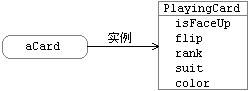
\includegraphics[scale=0.6]{playingcard_meta.png}
\label{fig:playingcard_meta}
\end{figure}


在Smalltalk语言中,类就是对象。类自身就是可以对特定消息作出响应,比如用来创建对象的消息new。例如,在下面所示的示意图显示了类自身对特定消息作出响应。


\begin{figure}[htbp]
\centering
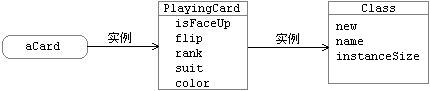
\includegraphics[scale=0.6]{smalltalk_meta.png}
\label{fig:smalltalk_meta}
\end{figure}

假设有这样一种情况,我们想要创建一个可以用在构造函数中的方法,即我们需要一种方法——假设为rank: suit:,它可以传递给具体的类对象——假设为PlayingCard,当执行方法时,将创建一个新的实例并确保这个实例被正确地初始化。在这种情况下,这个方法应该放在什么地方呢?它不可能是PlayingCard的成员方法,因为它是类实例所执行的方法,而在创建类的时候我们还没有实例。它也不是Class的成员方法,因为Class的成员方法对所有的类都是通用的,而这个初始化方法只是针对这一个类有效。

解决方案是创建一个新的“隐藏”类,称为元类(metaclass),名字为PlayingCard的对象实际上不是Class的实例,而是MetaPlayingCard的实例,而MetaPlayingCard则继承于Class。与初始化相关的特定行为可以置于这个元类中。


\begin{figure}[htbp]
\centering
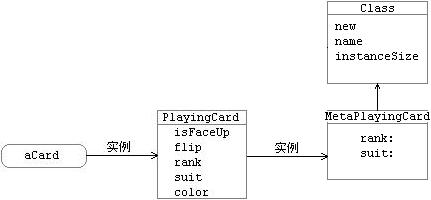
\includegraphics[scale=0.6]{acard_meta.png}
\label{fig:acard_meta}
\end{figure}

类MetaPlayingCard中的行为,只能被对象PlayingCard所理解,而不能被其他对象所理解。对象PlayingCard是类MetaPlayingCard的唯一实例。

Smalltalk浏览器通常对用户隐藏元对象,我们把这样的方法称为类方法(class method),它们看起来就像与类相关联一样,但是在浏览器背后,类方法只是和元类相关联的普通方法。


\begin{lstlisting}[language=C++]

\end{lstlisting}





\begin{lstlisting}[language=C++]

\end{lstlisting}




\chapter{Method}



\section{Overview}


关于纸牌抽象的进一步改进,包括以下几个方面:

\begin{compactitem}
\item 增加一种方法,可以返回纸牌的颜色(红色还是黑色);
\item 增加一个数据字段,来表示纸牌是面朝上还是面朝下,并且增加检测这一数据字段值状态的方法和翻转纸牌的方法。
\end{compactitem}


使用C\#定义的用来表明这些变化的一个典型的类如下所示:

\begin{lstlisting}[language={[Sharp]C}]
class PlayingCard{
	// constructor, initialize new playing card
	public PlayingCard(Suits is, int ir){
		suit = is;
		rank = ir;
		faceup = true;
	}
	
	// operations on a playing card
	public Boolean isFaceUp(){
		return faceup;
	}
	public Suits suit(){
		return suitValue;
	}
	public int rank(){
		return rankValue;
	}
	public void setFaceUp(Boolean up){
		faceUp = up;
	}
	public void flip(){
		setFaceUp(!faceUp);
	}
	public Color color(){
		if((suit() == Suits.Diamond) || (suit() == Suits.Heart))
			return Colors.Red;
		return Color.Black;
	}
	
	// private data values
	private Suits suitValue;
	private int rankValue;
	private Boolean faceUp;
}
\end{lstlisting}



其中,需要注意的特征就是增加了第二个枚举数据类型来表示颜色,并且又增加了以private来修饰的第3个数据字段来表示纸牌面朝上状态。

将数据字段声明为private意味着禁止从类定义的外部来存取该数据字段,从而确保了修改该数据字段的唯一方式就是使用与这个类相联系的方法。

大多数的面向对象编程方式指南都会建议,数据字段永远不应声明成public,而应该是private或者protected。

构造函数是一种特殊的方法,它们有着和类相同的名称,并且用于在对象中初始化数据字段。

\subsection{getter}


类必须对外提供一种存取数据字段的方法,通过定义于类中的方法来存取数据字段是一种好的面向对象编程方式。

仅仅返回数据字段值的方法称为存取器(accessor),有时也称为获取器(getter)。这里,getter方法的一个实例是isFaceUp,它返回数据字段faceUp的值。另外一个例子是方法rank,它返回数据字段rankValue的值。


为什么对这个简单的行为使用一个方法,而不是直接存取数据字段来实现呢?

一个原因就是方法可以使数据字段是只读的(read-only)。函数只能被调用,而数据字段既可以读又可以写,因此通过private数据字段和public存取器的结合,我们可以确保纸牌的点数一旦创建,就不会被改变。


这里所使用的对方法的命名是一种典型的命名约定。以is开头命名一个返回布尔值的方法是很好的做法,它清楚地表示了当方法返回真值时所代表的含义。按照这一约定,可以更容易理解条件语言中使用的方法,如下所示:

\begin{lstlisting}[language={[Sharp]C}]
if(aCard.isFaceUp())...
\end{lstlisting}


这里,aCard是PlayingCard类的一个实例。很多编程方式指南建议存取器方法以get这个词开始,这样可以清晰地表明,该方法最主要的目的仅仅是获取数据字段的值。这一约定也使得使用这种方法的语句更容易理解,如下所示:



\begin{lstlisting}[language={[Sharp]C}]
int cardRank = aCard.getRank();
\end{lstlisting}

然而,这一约定并不适用于任何情况,尤其是当为这些方法使用更简单的名称rank和suit时。

\subsection{setter}


主要目的仅仅是设置字段值的方法称为可变器(mutator)或者设置器(setter),设置器的命名通常以单词set开始。例如,方法setFaceUp就是设置器的一个实例,它用来设置存取器faceUp的值。


\begin{lstlisting}[language={[Sharp]C}]
class PlayingCard{
	...
	void setFaceUp(Boolean up){
		faceUp = up;
	}
	...
}
\end{lstlisting}

flip方法既不是获取器也不是设置器,因为它既没有获取数据字段值,也没有设置数据字段值。它只是一个简单的方法。方法color从技术上来说也不是获取器,因为它没有获得关于这个类的数据字段值。尽管如此,但由于它返回了对象的一个属性,所以一些编程指南建议,getColor是一个更好的命名。


Smalltalk语言不支持访问修饰符。

缺省情况下,Smalltalk语言中的所有数据字段都是private(即只能在类定义内部进行存取)。为了存取数据字段,必须提供相应的存取器方法:


\begin{lstlisting}[language=bash]
rank 
	" return the face value of a card "
	'$\uparrow$' rank
\end{lstlisting}



Smalltalk语言并没有广泛地遵循以单词get开始的命名约定。通常情况下,Smalltalk语言中存取器方法与它们返回的数据字段同名。

获取器和设置器函数(或者称为存取器和可变器),通过它们可以对数据字段进行存取,这样使用方法而不是直接存取数据字段,用户可以更加灵活地控制数据的修改方式以及确定数据所处的位置。


\section{Declaration}


一般说来,并不指定在类定义中方法的声明次序,不过次序对代码的可读性有很大的影响。

\begin{compactitem}
\item 在类定义中,首先列出一些主要的特征,一些次要的特征列在后面。
\item 构造函数是对象定义的一个最重要的方面,因此应该位于类定义的顶部。
\item 对方法的声明应该通过分组来表示,这样可以迅速便捷地找到对应于给定消息选择器的方法。分组的原则可以按照字母顺序排列,或者按照方法的职能进行分组。
\item 私有数据类型只是对于类的开发者才重要,它们应该列在类定义中靠后的位置。
\end{compactitem}


在面向对象编程中,消息总是传递给接收器。然而,在大多数面向对象语言中,接收器并不出现在方法的参数列表中,而是隐藏于方法的定义之中,也就是说用来响应消息的方法在方法体内部存取消息接收器。

只有当必须从方法体内部去存取接收器的数值时,才会使用伪变量(pseudo-variable)。伪变量和通常的变量很相似,只是它不需要声明,也不能被更改(因此这里也许使用伪常量更加合适,只是伪常量从未出现在任何语言的定义中)。

\begin{compactitem}
\item 在Java和C++语言中,由伪变量表示的接收器命名为this;
\item 在Eiffel语言中称为Current;
\item 在Smalltalk、Objective-C、Object Pascal等语言中称为self。
\end{compactitem}

伪变量在使用时就好像是作为类的一个实例。例如,方法color可以用Pascal语言编写成如下结果:

\begin{lstlisting}[language=Pascal]
function PlayingCard.color : colors;
begin
	if(self.suit = Heart) or (self.suit = Diamond) then
		color := Red
	else
		color := Black;
end
\end{lstlisting}

在很多编程语言中,对接收器伪变量的使用都可以忽略。如果在没有引用接收器的条件下,访问一个数据字段或者调用一个方法,那么这意味着接收器伪变量将作为消息的主体。

例如,PlayingCard中的flip方法就体现了这一点,flip方法就是通过调用setFaceUp方法来实现它的功能的:



\begin{lstlisting}[language=Java]
class PlayingCard{
	...
	public void flip(){
		setFaceUp(!faceUp);
	}
}
\end{lstlisting}

使用伪变量可以将这一方法重新编写,从而使接收器显示出来,如下所示:



\begin{lstlisting}[language=Java]
class PlayingCard{
	...
	public void flip(){
		this.setFaceUp(!this.faceUp)
	}
}
\end{lstlisting}

当某一方法想要把自身当作一个参数传递给另外一个函数时,就必须使用变量来解决问题。



\begin{lstlisting}[language=Java]
class QuitButton extends Button implements ActionListener{
	public QuitButton(){
		...
		//install ourselves as a listener for button events
		addActionListener(this);
	}
	...
}
\end{lstlisting}

对于构造函数,使用this和构造函数的参数初始化数据成员。通过显式地使用this,可以区分用作函数参数和数据成员的两个同名变量。


\begin{lstlisting}[language=Java]
class PlayingCard{
	public PlayingCard(int suit,int rank){
		this.rank = rank; //this.rank is the data member
		this.suit = suit; //rank is the argument value
		this.faceUp = true;
	}
	...
	private int suit;
	private int rank;
	private boolean faceUp;
}
\end{lstlisting}

Python、CLOS和Oberon等语言则不遵循上述原则,接收器必须在方法体中显式地声明。例如,在Python语言中,一条消息可以包含两个参数,如下所示:




\begin{lstlisting}[language=Python]
aCard.moveTo(27,3)
\end{lstlisting}

相应的方法需要声明3个参数值:


\begin{lstlisting}[language=Python]
class PlayingCard:
	def moveTo(self, x, y):
		...
\end{lstlisting}


对于这些语言,尽管原则上第一个参数可以以任何名称来命名,但是一般都命名为self或者this,以此来表示该方法与接收器伪变量之间的关系。

在CLOS和Oberon语言中,也必须把接收器命名为方法的一个参数。


\begin{lstlisting}[language=Java]

\end{lstlisting}




\begin{lstlisting}[language=Java]

\end{lstlisting}

\section{Constant}

一些编程语言提供了一种方式来作为存取器方法的一种替代,可以指定一个数据字段是可变的或者是不可变的,从而意味着如果设定了数据字段的值,就不能再改变它,就没有必要通过方法来隐藏对数据值的存取。


下面描述了关于定义常量的不同方式。例如,在Java中是用final来声明常量的,在C++中则使用修饰符const来实现。


\begin{lstlisting}[language=C++]
// C++
class PlayingCard{
public:
	...
	const int rank; // since immutable, can allow public access to data field.
	const Suits suit;
};
\end{lstlisting}


\begin{lstlisting}[language=Java]
// Java
class PlayingCard{
	...
	public final int rank;
	public final Suits suit;
}
\end{lstlisting}


常量(或者称为不可变数据字段)直观地说明了在程序执行过程中不能改变其值的数据字段。





\section{Isolation}

Java和C\#等都是把方法的主体直接放在类定义中,而C++和Object Pascal等语言则是将这两方面分离开来。

在C++语言中可以自由选择,小规模的方法可以在类内部定义,大规模的方法可以在类外部定义。例如,一个关于纸牌抽象的C++类定义如下所示:

\begin{lstlisting}[language=C++]
// C++ 
class PlayingCard{
public:
	enum Suits { Spade, Diamond, Club, Heart };
	enum Colors { Red, Black };
	// constructor, initialize new playing card
	PlayingCard(Suits is, int ir){
		suit = is;
		rank = ir;
		faceUp = true;
	}
	// operations on a playing card
	boolean isFaceUp(){ // bool
		return faceUp;
	}
	void setFaceUp(bool up){
		faceUp = up;
	}
	void flip(){
		setFaceUp(!faceUp);
	}
	int rank(){
		return rankValue;
	}
	Suits suit(){
		return suitValue;
	}
	
	Colors color();

private: // private data values
	Suits suitValue;
	int rankValue;
	boolean faceUp; // bool
};
\end{lstlisting}

注意,这里忽略了方法color的实现主体,因为它的实现代码比在类中所定义的其他方法都要长。随后的方法定义(又称为函数成员,function member)提供了函数的主体。


\begin{lstlisting}[language=C++]
// C++
PlayingCard::Colors PlayingCard::color(){
	// return the face color of a playing card
	if((suit == Diamond) || (suit == Heart))
		return Red;
	return Black;
}
\end{lstlisting}

方法标题定义的格式和通常的C语言函数定义十分类似,只是名称已经扩展成为一个全限定(fully qualified)名,而且这种受限定的名称由类的名称和定义的方法名称组成,如同一个人是由姓和名来确定的一样(例如“Jim Green”)。

C++程序员既可以将方法作为类定义的一部分,定义成内联(in-line)方法,也可以将方法定义成程序的一个独立的部分。

一般情况下,把只有一到两个语句的方法定义成内联方法,把多于两行的复杂语句定义在类的外部。



把方法体放在类定义之外有两个原因。首先,多余一条语句的方法体会使类定义的其他特征变得模糊,因此移开代码比较长的方法体可以改善程序的可读性。只是,可读性是针对观察者的,而不是所有的用户都认为这种分离可以提高程序的可读性,因为这样做之后,用户就必须到两个不同的地方去查找方法的主体。

第二个原因涉及到语义。当方法体在一个类定义内部被声明时,C++编译器就可以直接将其作为内联方法进行扩展,而无需建立函数调用,这样内联方法比函数调用和方法体的结合形式执行起来更加快速。


在C++语言程序中,通常不会在同一个文件中同时出现类定义和较大的方法体。

\begin{compactitem}
\item 类声明一般会在接口文件(interface file)中给出(按照惯例,在UNIX系统中是扩展名为.h的文件,在Windows系统中是扩展名为.hpp的文件)。
\item 函数体位于实现文件中(按照惯例,是扩展名为.cpp或.C的文件)。
\end{compactitem}

Objective-C语言也把类定义和类实现分离开来。其中,类定义包括关于类的方法的描述,它们通过符号“+”或者“-”来指示,随后紧接着位于括号之内的返回类型,返回类型之后是方法的描述。

\begin{lstlisting}[language={[Objective]C}]
@ interface PlayingCard : Object
{
	int suit;
	int rank;
	int faceUp;
}
	
+ suit: (int) s rank: (int) i
- (int) color;
- (int) rank;
- (int) suit;
- (int) isFaceUp;
- (void) flip;
@ end
\end{lstlisting}


关于方法体的实现代码如下:



\begin{lstlisting}[language={[Objective]C}]
@ implementation PlayingCard
	
- (int) color
{
	if((suit == Diamond)||(suit == Heart))
		return Red;
	return Black;
}
- (int) rank
{
	return rank;
}
... ./* other method bodies */
@ end
\end{lstlisting}



Object Pascal和Delphi语言分离类定义和方法函数体的方式很相似,分离的这两个部分都是保存在同一个文件中。类定义描述位于以interface为标识的部分,而具体实现代码位于以implementation为标识的部分。例如,下面就是一个Delphi语言的示例。


\begin{lstlisting}[language=C++]
interface
type
	Suits = (Heart,Club,Diamond,Spade);
	Colors = (Red,Black);
	
	TPlayingCard = class (TObject)
		public
			constructor Create (r : integer; s : Suits);
			function color : Colors;
			function isFaceUp : boolean;
			procedure flip;
			function rank : integer;
			function suit : Suits;
		private
			suit : Suits;
			rank : integer;
			faceUp : boolean;
	end;	
implementation
	function TPlayingCard.color : Colors;
	begin
		case suit of
			Diamond: color := Red;	
			Heart: color := Red;
			Spade: color := Black;
			Club: color := Black;
	end

...(* other methods similarly defined *)
end;
\end{lstlisting}



在Pascal语言中的全限定名是通过在类名和方法名之间使用句点分隔而成,C++语言则是使用冒号来进行分隔。

CLOS语言在进行类定义时,可以通过使用“:accessor”关键字和位于其后的存取器函数名,自动地创建存取函数。


\begin{lstlisting}[language=Lisp]
// CLOS
(defclass PlayingCard()
	((rank :accessor getRank) (suit :accessor getSuit) ))
\end{lstlisting}

其他的方法是使用函数defmethod来定义的,而且方法的接收器以一个显式参数来命名,这一点和Java以及C++语言是不同的。





\begin{lstlisting}[language=Lisp]
// CLOS
(defmethod color((card PlayingCard))
	(cond
		((eq (getSuit card) ‘Diamond) ‘Red)
		((eq (getSuit card) ‘Heart) ‘Red)
		(t 'Black)))
\end{lstlisting}

在Python语言中,接收器也必须以显示参数命名。




\begin{lstlisting}[language=Python]
class PlayingCard:
def __init__(self, s, r):
	self.suit = s
	self.r = r
def rank(self):
	return self.rank
def color(self):
	if self.suit == 1 or self.suit == 2:
		return 1
	return 0
\end{lstlisting}


\section{Message}


\begin{compactitem}
\item 面向对象语言的静态特征包括如何创建新的数据类型、新的类和新的方法等。
\item 面向对象语言的动态特征涉及到值是如何实例化(或者被创建)的,它们又是如何初始化的,以及它们如何通过消息传递来相互联系。
\end{compactitem}

在面向对象编程思想中,创建(实例化)就是为一个新对象分配存储空间并且将这段空间与对象名称进行绑定。

实际上,初始化不但包括为对象的数据区域设置初始值(类似于对记录中的数据字段进行的初始化),还包括建立操作对象所需的初始条件这个更一般的过程。

在大多数面向对象语言中,后者对于使用对象的客户的隐藏程度是封装的一个重要的方面,这也被认为是面向对象技术优于其他编程技术的一个主要方面。

使用消息传递(message passing,或称为method lookup,方法查询)这一术语来表示请求对象执行一项特定行为的动态过程。例如,在Fred送花给Cris的示例中,非正式地描述了消息传递,并且指明了如何区分消息和通常的过程调用。

\begin{compactitem}
\item 消息总是传递给某个称为接收器的对象;
\item 响应消息所执行的行为不是固定不变的,它们根据接收器类的不同而不同。
\end{compactitem}

不同的对象可以接收相同的消息,但是却执行不同的行为,因此对于任何消息传递表达式都有3个确定的部分,它们是接收器(receiver,消息传递的目的对象)、消息选择器(message selector,表示待传递的特定的消息文本)和用于响应消息的系数(argument)。

\begin{figure}[htbp]
\centering
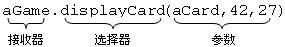
\includegraphics[scale=0.65]{message.png}
\caption{消息传递表达式}
\label{fig:message}
\end{figure}

消息传递最通常的语法是使用句点来把接收器和消息选择器分离开来,还有一些次要的变化特征。例如,在方法没有参数时,是否需要使用一对空的圆括号(在Pascal和一些其他的语言中可以省略这对圆括号)。

\begin{lstlisting}[language=C]
// C++, C#, Java, Python, Ruby
aCard.flip();
aCard.setFaceUp(true);
aGame.displayCard(aCard,45,56);
// Pascal, Delphi, Eiffel, Oberon
aCard.flip;
aCard.setFaceUp(true);
aGame.displayCard(aCard,45,56);
// Smalltalk
aCard flip.
aCard setFaceUp: true.
aGame display: aCard atLocation: 45 and: 56.
// Objective-C
[ aCard flip ].
[ aCard setFaceUp: true ].
[ aGame display: aCard atLocation: 45 and: 56 ]
// CLOS
(flip aCard)
(setFaceUp aCard true)
(displayCard aGame 45 56)
\end{lstlisting}

在Smalltalk和Object-C语言中,表示消息传递的语法有一些细微的差异,使用空格作为分隔符。一元消息(不含参数的消息)只是简单地写在接收器之后。含有参数的消息使用关键字表示法(keyword notation)。消息选择器被分成几个部分,每个参数之前都有一个部分。冒号跟在每个关键字之后。

\begin{lstlisting}[language=C++]
aGame display: aCard atLocation: 45 and: 56.
\end{lstlisting}


在Smalltalk语言中,即使是二元操作(例如加法)也被解释为将右值参数传递给左值的消息。

\begin{lstlisting}[language=C++]
z <- x + y. " message to x to add y to itself and return sum "
\end{lstlisting}

在C++语言中定义的二元操作符也表示相似的含义。

在Object-C语言中,将一条类似于Smalltalk语言的消息包含在方括号中,称为消息传递表达式。方括号只包括消息本身,而不包括其他内容。例如,不包括存放消息结果的变量。


\begin{lstlisting}[language=C++]
int cardrank = [ aCard getRank ];
\end{lstlisting}


CLOS语言中的语法遵循传统的Lisp语法。Lisp语言中的所有表达式都写成以圆括号为边界的列表。操作是列表的第一个元素,紧接着是参数。接收器是第一个参数。

\section{Friend}

在某些情况下,用户可以通过被重载的操作符等来允许特定的非成员函数访问一个类的私有成员,同时仍然阻止一般地访问。例如,用户可以重载输入/输出操作符(>>和<<)来访问类的私有数据成员,而且这些操作符不可能是类的成员,但是它们仍然是类的“接口的组成部分”。

C++语言的友元(friend)机制允许一个类将对其非公有成员的访问权授予指定的函数或类。

友元的声明以关键字friend开始,只能出现在类定义的内部,并且不受其声明位置的访问控制影响,因此通常将友元声明成组地放置在类定义的开始或结尾。

在下面的示例中,窗口管理器类Window管理给定显示器上的一组Screen,在逻辑上Window类可能需要访问由其管理的Screen对象的内部数据。



\begin{lstlisting}[language=C++]
class Screen{
	// Window members can access private parts of class Screen
	friend class Window;
	// ...
};
\end{lstlisting}

友元可以是普通的非成员函数,或其他类的成员函数,或者整个类。例如,在将一个类设为友元时,友元类的所有成员函数都可以访问授予友元关系的类的非公有成员。

这里,与Screen类是友元关系的Window类的成员就可以直接引用Screen的私有成员。例如,Window提供了一个函数来重定位一个Screen。


\begin{lstlisting}[language=C++]
Window&
Window::relocate(Screen::index r, Screen::index c, Screen& s)
{
	// refer to height and width
	s.height += r;
	s.width = c;
	return *this;
}
\end{lstlisting}

另外,用户也可以使用函数所属的类的方式来指定只允许特定的成员函数访问类的成员。

\begin{lstlisting}[language=C++]
class Screen{
	// Window must be defined before class Screen
	friend Window& Window::relocate(Window::index, Window::index, Screen&);
	// ...
};
\end{lstlisting}

为了正确地构造类,需要注意友元声明与友元定义之间的相互依赖,因此必须在定义包含成员函数的类之后才能将其成员函数设为友元。不过,不必预先声明类和非成员函数来将它们设为友元。

友元声明将已命名的类或非成员函数引入到外围作用域中,友元函数可以在类的内部定义,而且友元函数的作用域扩展到包围包围类定义的作用域。

使用友元引入的类名和函数(定义或声明)可以和类本身预先声明的一样使用。

\begin{lstlisting}[language=C++]
class X{
	friend class Y;
	friend void f(){}
};
class Z{
	Y *ymem;
	void g(){return ::f();}
};
\end{lstlisting}

类必须将重载函数集中在每一个希望设为友元的函数都声明为友元。

\begin{lstlisting}[language=C++]
extern std::ostream& storeOn(std::ostream &, Screen &);
extern BitMap& storeOn(BitMap &, Screen &);
class Screen{
	// ostream version of storeOn may access private parts of Screen objects
	friend std::ostream& storeOn(std::ostream &, Screen &);
	// ...
};
\end{lstlisting}



\chapter{Property}



\section{Overview}

编程语言(包括面向对象语言和非面向对象语言)都包含一种称为属性的概念。在语法上,属性是以数据字段的方式来进行操作的,但是像方法一样,它也是内部操作。也就是说,属性既可以作为表达式来读取,也可以对其进行赋值。




\begin{lstlisting}[language=C++]
Writeln('rank is', aCard.rank); (* rank is property of card *)
aCard.rank = 5; (* changing the rank property *)
\end{lstlisting}

无论是读取属性值还是对属性赋值,都必须通过函数来实现,而不是仅仅由一个简单的数据值来实现。

Delphi语言中的属性是通过关键字property以及修饰符read和write来声明的,紧跟read和write关键字之后的可以是数据字段,也可以是方法名。

当某一属性用在表达式的形式中,read属性就会被会调用,而当属性作为赋值目标时,write属性就会被调用。只能读取而不能写入的属性称为只读属性。

例如,在下面的示例中,对属性的修改作为属性的纸牌点数值和花色值。







\begin{lstlisting}[language=C++]
type
	TPlayingCard = class(TObject)
		public
				
			property rank : Integer read rankValue;
			property suit : Suits read suitValue write suitValue;
		private
			rankValue : Integer;
			suitValue : Suits;
	end;
\end{lstlisting}

这里,我们把点数定义成只读属性,而将花色定义成读写属性,也可以定义一个只写属性,只是这很少用。


在C\#中,属性是通过编写一个无参数的方法来定义的,这个方法只包括一个get部分或者一个set部分,其中:

\begin{compactitem}
\item get部分必须返回一个值;
\item set部分可以使用伪变量value来设置属性。
\end{compactitem}

\begin{lstlisting}[language={[Sharp]C}]
public class PlayingCard{
	public int rank{
		get{
			return rankValue;
		}
		set{
			rankValue = value;
		}
	}
	...
	private int rankValue;
}
\end{lstlisting}

\begin{compactitem}
\item 如果只有get部分而没有提供set部分,则属性为只读属性。
\item 如果只有set部分而没有提供get部分,则属性为只写属性。
\end{compactitem}

在C\#程序中,属性通常是无参数且返回惟一值的函数。





\subsection{C++}


\begin{lstlisting}[language=C++]

\end{lstlisting}




\subsection{Java}


\begin{lstlisting}[language=C++]

\end{lstlisting}



\subsection{C\#}



\begin{lstlisting}[language=C++]

\end{lstlisting}

\section{Mutable}

如果希望类的数据成员(包括在const成员函数内)可以修改,可以将它们声明为mutable。

可变数据成员永远都不能为const,因此const成员函数可以改变mutable成员,需要使用关键字mutable来声明数据成员。

\begin{lstlisting}[language=C++]
class Screen{
public:
// interface member functions
private:
	mutable size_t access_ctr; // may change in const members
	// other data members as before
};
\end{lstlisting}



\section{Static}



对于特定类类型的全体对象而言,访问一个全局对象有时是必要的。例如,在程序的任意点需要统计已创建的对象的数量,或者全局对象可能是指向类的错误处理例程的一个指针,或者全局对象是指向类类型对象的内存自由存储区的一个指针。

全局对象的问题在于它可能会破坏封装,对象需要支持特定类抽象的实现,因此类可以定义类静态成员来提供全局对象的功能。


\begin{compactitem}
\item 非static数据成员存在于类类型的每个对象中。
\item static数据成员独立于类的任意对象而存在。
\end{compactitem}

用户可以在类的成员声明前加上关键字static来定义static数据成员和static成员函数,而且static成员遵循正常的公有/私有访问规则。


\begin{compactitem}
\item static数据成员是与类关联的对象,并不与类的对象相关联。
\item static成员函数没有this形参,它可以直接访问所属类的static成员,但是不能直接使用非static成员。
\end{compactitem}

相比全局对象,static成员具有如下三个优点:

\begin{compactenum}
\item static成员的名字在类的作用域中,可以避免与其他类的成员或全局对象名字冲突。
\item static成员可以是私有成员,因此可以实施封装,但是全局对象不可以。
\item static成员与特定类关联。
\end{compactenum}

例如,在设计一个简单的表示银行账户的类时,每个账户具有余额和所有人,并且按月计算利息,不过应用于每个账户的利率总是相同的。

\begin{lstlisting}[language=C++]
class Account{
public:
	// interface functions
	void applyint() { amount += amount * interestRate; }
	static double rate(){ return interestRate; }
	static void rate(double); // sets a new rate
private:
	std::string owner;
	double amount;
	static double interestRate;
	static double initRate();
};
\end{lstlisting}

用户可以通过作用域操作符从类直接调用static成员,或者通过对象、引用或指向该类类型对象的指针间接调用。

\begin{lstlisting}[language=C++]
Account ac1;
Account *ac2 = &ac1;
// equivalent ways to call the static member rate function
double rate;
rate = ac1.rate();
rate = ac2->rate();
rate = Account::rate();
\end{lstlisting}

\subsection{Static Method}

在类的外部定义static成员时,无须重复指定static保留字,而且该保留字只出现在类定义体内部的声明处。

\begin{lstlisting}[language=C++]
void Account::rate(double newRate)
{
	interestRate = newRate;
}
\end{lstlisting}

static成员是类的组成部分但不是任何对象的组成部分,因此static成员函数没有this指针,如果使用非static成员显式或隐式地引用this将导致编译时错误。

static成员不是任何对象的组成部分,因此static成员函数不能被声明为const,也不能被声明为虚函数。

\subsection{Static Member}

static数据成员可以声明为任意类型,可以是常量、引用、数组、类类型等,不过static数据成员必须在类定义体的外部定义(正好一次\footnote{在实际开发中,保证对象正好定义一次的最好办法就是将static数据成员的定义放在包含类的非内联成员函数定义的文件中。})。

与普通数据成员不同,static成员不通过类的构造函数进行初始化,而且需要在定义时进行初始化。

在类定义体外部引用类的static成员时,必须指定成员是在哪个类中定义的,static关键字只能用于类定义体内部的声明中,定义不能标示为static。

一般情况下,类的static成员不能在类的定义体中声明时进行初始化,通常只有在定义时才初始化。不过,只要初始化式是一个常量表达式,那么整型const static数据成员就可以在类的定义体中进行初始化,但是const static数据成员仍然必须在类的定义体外部进行定义。



\begin{lstlisting}[language=C++]
class Account{
public:
	static double rate(){ return interestRate; }
	static void rate(double); // sets a new rate
private:
	static const int period = 30; // interest posted every 30 days
	double daily_tbl[period];
};
\end{lstlisting}

这里,使用常量值初始化的整型const static数据成员就是一个常量表达式,它也可以用于任何需要常量表达式的地方。


在类内部提供初始化式时,成员的定义不必再指定初始值。

\begin{lstlisting}[language=C++]
// definition of static member with no initializer
// the initial value is specified inside the class definition
const int Accout::period;
\end{lstlisting}



\chapter{Field}

使用被一个类的所有实例共享的公共数据字段,在解决许多问题时都非常方便。然而,对这样的对象进行的操作却为面向对象语言的设计者创建了一个奇特的矛盾。

为了理解这个问题,考虑一下当初创建类这个概念的原因——就是要减少创建相似对象的工作量。类的每一个实例都和这个类的其他实例有着完全一致的行为。现在,假设由于某种原因我们定义了一个公共数据字段,它可以被类的所有实例共享,然后考虑如何对公共数据字段进行初始化。这看起来有两种选择,但是每种选择都不能令人满意。一种选择是每个实例都执行对公共数据字段的初始化任务(字段初始化后,还会被反复地初始化),另一种选择是没有实例执行初始化任务(数据字段一直处于未初始化状态)。

为了解决这一矛盾,我们需要从类/方法/实例这个简单的实例中跳出来进行思考,因此另外一个机制就是,对象本身不必对共享数据进行初始化。

如果对象通过内存管理器自动将共享数据初始化为一个特定值(例如0),那么每一个实例都可以测试这一特定值,并且如果它们是第一个进行测试的实例,它们就会对数据进行初始化。不过,还应该有其他的更好的方法。

在C++和Java语言中,共享数据字段都是使用static修饰符来创建的。例如,在Java语言的符号常量创建中,就会使用这种办法。

一般情况下,Java语言中的静态数据字段的初始化是在加载类时,通过执行静态块(static block)来完成的。例如,假设我们想要了解一个类已经创建了多少个实例,可以通过下面的方法来实现。

\begin{lstlisting}[language=Java]
class CountingClass{
	CountingClass(){
		count = count + 1; // increment count
		...
	}
	...
	private static int count; // shared by all
	static { // static block
		count = 0;
	}
}
\end{lstlisting}

C++语言有两种不同的方法,其中由基本数据类型表示的静态数据字段(或常量)可以在类的主体中进行初始化,或者也可以在类之外对静态数据字段进行全局的初始化。



\begin{lstlisting}[language=C++]
class CountingClass{
pubilc:
	CountingClass(){
		count ++;
		...
	}

private:
	static int count;
};

// global initialization is separated from class
int CountingClass::count = 0;
\end{lstlisting}

C\#语言可以通过静态构造方法(声明为static的构造方法)来对静态数据字段进行初始化,而且构造方法不允许有任何参数。


使用关键字static就解决了以前关于初始化一个类的所有实例共享数据字段所引起的特殊矛盾。

Python语言中的类的数据字段在方法层次上命名,而实例变量在方法内部命名(一般在构造方法内部)。

\begin{lstlisting}[language=Python]
class CountingClass:
	count = 0
	def __init__(self):
		self.otherField = 3
\end{lstlisting}



\section{Anonymous Class}

在很多面向对象语言中,类本身就是一个对象。

在多数情况下,有一个特殊的类(一般称为Class),这就是类的类,而且它们具有相应的行为。例如,通常创建类的一个实例就是简单地给类对象传递一条消息。




下面是Smalltalk中的相应示例:

\begin{lstlisting}[language=C++]
aCard<-PlayingCard new. "message new given to object PlayingCard"
\end{lstlisting}

其他的一般行为包括返回类的名称、类实例大小或者类实例可识别的消息列表。

在非交互式语言中,有时很难表示程序语句和程序输出之间的关系,在实际的程序开发中要能够区分可执行语句和非执行的输出结果。例如,下面的Java代码就说明了这些应用:




\begin{lstlisting}[language=C++]
Object obj = new PlayingCard();
Class c = obj.getClass();
System.out.println("class is " + c.getName());
\end{lstlisting}

至于类是否是面向对象编程所必需的,现代软件开发技术中已经证明,不使用类而通过委托(delegation)就可以实现面向对象语言的大多数期望的特征。

不过,从委托语言的第一次提出到现在,它并没有得到完全支持,所以大多数用户更愿意使用类。


\subsection{Java}

在某些应用场景中,用户需要创建一个简单的、不多于一个实例的类,这样的对象称为单件(singleton)。


Java提供了创建这样的对象的一种机制,甚至不需要对这样的对象所涉及的类进行命名,因此这样的类称为匿名类(anonymous class)。

为了创建匿名类,需要以下几个条件:

\begin{compactenum}
\item 只能创建一个匿名类的实例;
\item 匿名类必须继承于父类或接口,并且不需要构造函数进行初始化。
\end{compactenum}

在GUI(用户界面)的环境下,经常会遇到这种情况。例如,我们在设计一个用于创建图形按钮的类ButtonAdapter时,为了提供关于按钮的行为,程序员必须建立一个继承于ButtonAdapter的新类,并且改写方法pressed。

如果只需要一个这种对象,可以通过匿名类(又叫类定义表达式,class definition expression)来完成。

在使用方法add将图形元素添加到窗口时,为了将新按钮添加到窗口中,需要以下代码:


\begin{lstlisting}[language=Java]
Window p = ...
p.add(new ButtonAdapter("Quit"){
		public void pressed(){System.exit(0);}
	}
);
\end{lstlisting}

通过查看传递给add操作符的参数,会发现参数涉及一个新值的创建,通过add操作符来实现。

但是,这个关于new的参数列表的表达式并没有以反括号结束,而是又出现了一个花括号。实际上,这是一个新类的定义。创建了一个基于ButtonAdapter的子类,并且创建了一个关于这个子类的实例。这个新类所需的所有方法都通过内联函数给出。

在这个实例中,新类改写了名为pressed的方法,最后通过反花括号结束了匿名类表达式。


\chapter{Constructor}


\section{Overview}


构造函数(construtor)是用来初始化一个新创建对象的成员函数,而且构造函数本身可以重载\footnote{构造函数和普通函数一样,可以为一个类声明的构造函数的数量没有限制,而且可以没有形参,也可以定义多个形参,区别只是构造函数不能指定返回类型。}。

\begin{compactitem}
\item 构造函数用于给每个数据成员设置适当的初始值;
\item 构造函数应用初始化列表来初始化对象的数据成员。
\end{compactitem}

只要用户创建类类型的新对象,就需要执行构造函数,因此构造函数的作用就是在创建类类型的对象时保证每个对象的数据成员获得合适的初始值。

例如,在下面类定义中,构造函数Sales\_item()使用其初始化列表来初始化units\_sold和revenue成员,isbn成员由string的默认构造函数隐式初始化为空串。


\begin{lstlisting}[language=C++]
class Sales_item{
public:
	// operations on Sales_item objects
	// default constructor needed to initialize members of built-in type
	Sales_item(): units_sold(0), revenue(0.0) { }
private:
	std::string isbn;
	unsigned units_sold;
	double revenue;
};
\end{lstlisting}


构造函数的初始化列表由成员名和带括号的初始值组成,跟在构造函数的形参表后面,并以冒号开头。

\begin{lstlisting}[language=C++]
// default constructor needed to initialize members of built-in type
Sales_item(): units_sold(0), revenue(0.0) {}
\end{lstlisting}

只要每个构造函数的形参表是唯一的,那么可以为一个类声明的构造函数的数量没有限制,而且不同的构造函数允许用户指定不同的方式来初始化数据成员。

\begin{lstlisting}[language=C++]
class Sales_item{
// other members as before
public:
	// added constructors to initialize from a string or an istream
	Sales_item(const std::string&);
	Sales_item(std::istream&);
	Sales_item();
};
\end{lstlisting}


用户只有把创建和初始化联系起来才可以确保对象在正确地初始化之前不会被使用。假设创建和初始化分离时或者说没有构造函数,那么用户在创建新对象之后,可能就很容易忘记调用初始化例程,这样通常会导致不良后果。

在同一个对象上调用两次初始化过程,通常也会引起一定的麻烦,通过使用构造函数就可以避免这个问题。

构造函数的名字与类的名字相同,并且不能指定返回类型,构造函数执行两项主要任务—内存分配和初始化,从而确保所有得以分配内存的对象都可以被正确地初始化。

Java和C++语言可以通过检查与类显示的名称是否相同来识别构造函数和普通方法的区别,而且在定义新对象时传递给构造函数的实参决定了使用指定的构造函数。


另外,构造函数和普通方法的另一个细微的区别是构造函数不声明返回值的数据类型。

\begin{lstlisting}[language=Java]
class PlayingCard{ // a Java constructor
	public PlayingCard(int s, int r){
		suit = s;
		rank = r;
		faceUp = true;
	}
	...
}
\end{lstlisting}


当使用new操作符进行内存分配时,构造函数所需的参数紧随在类名之后,而且编译器会自动调用对应的构造函数。


\begin{lstlisting}[language=Java]
aCard = new PlayingCard(PlayingCard.Diamond, 3);
\end{lstlisting}

在Java和C\#语言中,数据字段可以初始化为特定的数值,这种赋值独立于构造函数中的参数赋值,数据字段可以在初始化时进行赋值,也可以在后来的构造函数中再次赋值。



\begin{lstlisting}[language=Java]
class Complex{ // complex numbers
	public Complex(double rv){
		realPart = rv;
	}
	public double realPart = 0.0; // initialize data areas to zero
	public double imgPart = 0.0; // initialize data areas to zero
}
\end{lstlisting}

在C++语言中,也使用类似的语法来声明静态(static)数据变量和/或常量(const),但是构造函数不能声明为const。


\begin{lstlisting}[language=Java]
class Sales_item{
public:
	Sales_item() const; // error
};
\end{lstlisting}

当创建类类型的const对象时就会执行一个普通构造函数来初始化产生的const对象,因此定义const构造函数是不必要的,而且实际上不管对象是否为const都使用同一个构造函数来初始化对象。


另外,C++、C\#和Java语言中只要每个函数参数的数目、类型或次序不同,就允许多个函数使用相同的名称定义,因此构造函数也使用重载方式进行定义。例如,一个构造函数为无参数函数,而另一个构造函数为有参数函数。


\begin{lstlisting}[language=C++]
class PlayingCard{
public:
	PlayingCard(){ // default constructor
		// used when no arguments are given
		suit = Diamond;
		rank = 1;
		faceUp = true;
	}
	
	PlayingCard(Suit is){ // constructor with one argument
		suit = is;
		rank = 1;
		faceUp = true;
	}
	
	PlayingCard(Suit is, int ir){ // constructor with two arguments
		suit = is;
		rank = ir;
		faceUp = true;
	}
};
\end{lstlisting}


参数数目、类型和次序的结合一般称为函数类型签名(type signature),通过检查调用的类型签名可以决定选择哪个过载构造函数。


\begin{lstlisting}[language=C++]
PlayingCard cardOne; // invokes default
PlayingCard *cardTwo = new PlayingCard;
PlayingCard cardThree(PlayingCard.Heart);
PlayingCard *cardFour = new PlayingCard(PlayingCard.Spade, 6);
\end{lstlisting}

必须注意的是,在C++语言中调用缺省构造函数时必须去掉括号。这里,使用括号虽然符合语法,但却有着完全不同的意义。



\begin{lstlisting}[language=C++]
PlayingCard cardFive; // create a new card
// forward definition for function 
// named cardSix that returns a PlayingCard
PlayingCard cardSix(); 
\end{lstlisting}

另外,当在C++语言中使用new操作符和无参数构造函数建立对象时,不需要括号,但是在Java和C\#语言中却完全相反。


\begin{lstlisting}[language=Java]
PlayingCard cardSeven = new PlayingCard(); // Java
PlayingCard *cardEight = new PlayingCard; // C++
\end{lstlisting}


\subsection{Initializer}



在C++语言中,构造函数可以使用与其他语言稍有不同的语法初始化数据成员,并且可以将这种冒号后跟着变量名称和括号括起来的初始值所组成的数据成员列表称为初始化器(initializer)。


\begin{lstlisting}[language=C++]
class PlayingCard{
public:
	PlayingCard(Suits is, int ir){
		:suit(is), rank(ir), faceUp(true){}
		...
	}
};
\end{lstlisting}

对于针对整数等简单数值,使用初始化器与在构造函数体中使用赋值语句是没有区别的。但是,还有其他各种不同形式的初始化,只能通过C++语言中的初始化器来实现。


\begin{lstlisting}[language=C++]
// recommanded way to write constructors using a constructor initializer
Sales_item::Sales_item(const string &book):
	isbn(book), units_sold(0), revenue(0) {}
\end{lstlisting}

构造函数和普通函数一样都可以定义在类的内部或外部,而且构造函数初始化器只在构造函数的定义中而不是声明中指定。

在使用C++语言定义的类中,省略初始化器并在构造函数的函数体内对数据成员赋值是合法的。例如,下面是一个接受一个string的Sales\_item构造函数的改写形式:

\begin{lstlisting}[language=C++]
// legal but sloppier way to write the constructor
// no constructor initializer
Sales_item::Sales_item(const string &book){
	isbn = book;
	units_sold = 0;
	revenue = 0.0;
}
\end{lstlisting}



在Objective-C语言中,构造函数不需要与类同名,它们可以通过使用位于函数定义之前的加号“+”而非减号“-”来标识。这样的函数称为工厂方法(factory method)。工厂方法使用new操作符执行实际的内存分配,然后执行初始化对象所需的所有行为。

\begin{lstlisting}[language={[Objective]C}]
@ implementation PlayingCard
+ suit: (int) s rank: (int) r{
	self = [ Card new ];
	suit = s;
	rank = r;
	return self;
} 
@ end
\end{lstlisting}

对于Objective-C语言,调用工厂方法是通过使用作为接收器的类来实现的,而不是使用实例对象。

\begin{lstlisting}[language={[Objective]C}]
PlayingCard aCard = [ PlayingCard suit : Diamond rank : 3 ];
\end{lstlisting}

在Python语言中,构造函数都有一个关键字“\_\_init\_\_”,当创建一个对象时,初始化函数是隐式调用的,传递的参数包括新创建的对象,以及其他用于创建表达式的参数。

\begin{lstlisting}[language=Python]
aCard = PlayingCard(2,3)
	# invokes PlayingCard.__init__(aCard, 2, 3)
\end{lstlisting}

在Apple Object Pascal语言中,没有构造函数,只能通过使用操作符new来创建新对象,用户通常定义他们自己的初始化例程,并且通过将新创建的对象作为接收器来调用初始化例程。

Object Pascal语言的Delphi版本和C++语言十分接近。与C++语言不同的是,Delphi用户不必将构造函数定义为和类同名,通常(但不是必需的)构造函数命名为Create。

\begin{lstlisting}[language=Delphi]
interface
	type
		TPlayingCard = class (TObject)
			constructor Create(is : Suits, ir : integer);
			...
		end;
	implementation
		constructor TPlayingCard.Create(is : Suits, ir : integer);
		begin
			suit = is;
			rank = ir;
			faceUp = true;
		end;
\end{lstlisting}

以类作为接收器,通过使用构造方法就可以创建对象。

\begin{lstlisting}[language=Delphi]
aCard := TPlayingCard.Create(Spade, 4);
\end{lstlisting}


正统规范的类(orthodox canonical class)形式要求几乎所有的类都应该定义4个重要的函数,如下所示:

\begin{description}
\item[缺省构造函数] 当建立的对象没有指定参数值时调用的构造函数,用于在内部初始化对象和数据成员。
\item[拷贝构造函数] 在实现按赋值参数调用(call-by-value parameter)时使用。
\item[赋值操作符] 用来把一个值赋给另外一个对象。
\item[析构函数] 当对象被删除时调用此函数。
\end{description}

缺省构造函数仅仅是一个无参数构造函数,拷贝构造函数以一个类实例的引用作为参数,并将对象自身初始化为参数的拷贝。



\begin{lstlisting}[language=C++]
class PlayingCard{
public:
	...
	PlayingCard(PlayingCard &aCard){
		// initialize ourself as copy of argument
		rank = aCard.getRank();
		suit = aCard.getSuit();
		faceUp = aCard.isFaceUp();
	}
	...
};
\end{lstlisting}


对于这四个函数,如果用户没有提供相应函数的实现,系统就会自动创建相应函数的缺省版本。

在大多数情况下(尤其是涉及动态内存分配时),缺省版本的实现并不是用户所希望的。即使没有完成类主体的编写,只提供这些函数的空壳,也表明程序设计者已经考虑了关于这些函数的问题。

此外,访问修饰符的合理使用使用户可以自由掌握允许或禁止某个类的各种不同操作。

在某些语言(比如C++和Java)允许创建只能赋值一次,禁止再做改变的数据字段。其中,Java语言将不可改变的数据字段声明为final,它可以直接进行初始化。




\begin{lstlisting}[language=Java]
class ListofImportantPeople{
	public final int max = 100; // maximum number of people
	...
}
\end{lstlisting}

或者,final值也可以在构造函数赋值。如果有多个构造函数,那么每一个构造函数都必须初始化这一数据字段。



\begin{lstlisting}[language=Java]
class PlayingCard{
	public PlayingCard(){
		suit = Diamond;
		rank = 1;
		faceUp = true;
	}
	public PlayingCard(Suits is, int ir){
		suit = is;
		rank = ir;
		faceUp = true;
	}
	...
	
	public final Suits suit; // suit and rank are immutable
	public final int rank; // 
	private boolean faceUp; // faceUp is not
}
\end{lstlisting}

在C++语言中,不可改变的值使用关键字const来标识,通过在构造函数中使用一个初始化子句来对其进行赋值。


\begin{lstlisting}[language=C++]
class PlayingCard{
public:
	PlayingCard() : suit(Diamond), rank(1){
		faceUp = true;
	}
	PlayingCard(Suits is, int ir) : suit(is), rank(ir){
		faceUp = true;
	}
	...
	
	const Suits suit;
	const int rank;
private:
	boolean faceUp;
};
\end{lstlisting}

在const和final这两种常数之间有一点细微但却十分重要的区别。

\begin{compactitem}
\item 在C++语言中,修饰符const说明的相关值是真正的常数,不允许改变。
\item 在Java语言中,修饰符final只是断言相关的变量不会赋予新值,没有什么能够阻止在对象内部对变量值进行改变(例如对消息的响应)。
\end{compactitem}

为了说明这一点,将下面的数据类型定义命名为Box:

\begin{lstlisting}[language=Java]
class Box{
	public void setValue(int v);
	public int getValue(){
		return v;
	}
	private int v = 0;
}
\end{lstlisting}

使用final声明一个变量,只是意味着它不会被重新赋值,并不意味着它不会再改变。



\begin{lstlisting}[language=Java]
final aBox = new Box(); //can be assigned only once
aBox.setValue(8); //but can change
aBox.setValue(12); //as often as you like
\end{lstlisting}

在C++语言中,使用const修饰符声明的变量禁止以任何方式进行修改,即使是处于对象的内部状态(个别的数据字段可以命名为mutable,这时即使数据字段处于一个常量对象内,也可以进行改变,只是这种情况很少见)。


\subsection{Sequence}

只要定义一个对象时没有提供初始化式,就会使用默认构造函数,而且为所有形参提供默认实参的构造函数也定义了默认构造函数。

\begin{compactitem}
\item 只有当一个类没有定义构造函数时,编译器才会自动生成一个默认构造函数。
\item 只要一个类定义了一个构造函数,编译器就不会再生成默认构造函数。
\end{compactitem}

构造函数初始化器仅指定用于初始化成员的值,并不指定初始化执行的次序,因此每个成员在构造函数初始化器中只能出现一次,而且被初始化的次序就是定义成员的次序。

在某些情况下,默认构造函数是由编译器隐式应用的,如果类没有默认构造函数,则该类就不能用在这些环境中,类通常应该定义一个默认构造函数。

实际上,如果定义了其他构造函数,则提供一个默认构造函数几乎总是对的,通常在默认构造函数中给成员提供的初始值应该指出该对象是“空”的。

假定有一个NoDefault类,它没有定义自己的默认构造函数,不过有一个接受一个string实参的构造函数,NoDefault类没有默认构造函数就意味着:

\begin{compactenum}
\item 具有NoDefault成员的每个类的每个构造函数,必须通过传递一个初始的string值给NoDefault构造函数来显式地初始化NoDefault成员。
\item 编译器不会为具有NoDefault类型成员地类合成默认构造函数,如果需要提供默认构造函数就必须显式地定义,并且默认构造函数必须显式地初始化其NoDefault成员。
\item NoDefault类型不能用作动态分配数组地元素类型。
\item NoDefault类型的静态分配数组必须为每个元素提供一个显式的初始化式。
\item 存储NoDefault对象的容器(例如vector)不能使用接受容器大小而没有同时提供一个元素初始化式的构造函数。
\end{compactenum}



除非一个成员根据其他成员来进行初始化,否则成员初始化的次序是无关紧要的,因此应该尽量按照与成员声明一致的次序编写构造函数初始化器,并且尽可能避免使用成员来初始化其他成员。

一般情况下,通过(重复)使用构造函数的形参而不是使用对象的数据成员,可以避免由初始化式的执行次序引起的任何问题。

合成的默认构造函数(synthesized default constructor)使用与变量初始化相同的规则来初始化成员。

\begin{compactitem}
\item 具有类类型的成员通过运行各自的默认构造函数来进行初始化。
\item 内置和复合类型的成员(例如指针和数组)只对定义再全局作用域中的对象进行初始化。
\item 当对象定义在局部作用域中时,内置或复合类型的成员不进行初始化。
\end{compactitem}

如果类包含内置或复合类型的成员,则该类不应该依赖于合成的默认构造函数,而是应该定义自己的构造函数来初始化这些成员。

此外,每个构造函数应该为每个内置或复合类型的成员提供初始化式,没有初始化内置或复合类型成员的构造函数,将使那些成员处于未定义的状态。

除了作为赋值的目标之外,以任何方式使用一个未定义的成员都是错误的。如果每个构造函数将每个成员设置为明确的已知状态,则成员函数可以区分空对象和具有实际值的价值。


初始化式可以是任意表达式,在指定实参并传递给成员类型时,可以使用对应的任意构造函数。

\begin{lstlisting}[language=C++]
Sales_item(const std::string &book, int cnt, double price):
	isbn(book), units_sold(cnt), revenue(cnt * price) { }
\end{lstlisting}

\subsection{Casting}

\begin{compactitem}
\item 为了定义到类类型的隐式转换,需要定义合适的构造函数,可以使用单个实参来调用的构造函数就定义了从形参类型到类类型的隐式转换。
\item 为了抑制由构造函数定义的隐式转换,可以通过将构造函数声明为explicit来防止在需要隐式转换的上下文中使用构造函数。
\end{compactitem}




\begin{lstlisting}[language=C++]
class Sales_item{
public:
	// default argument for book is the empty string
	explicit Sales_item(const std::string &book=""):
		isbn(book), units_sold(0), revenue(0.0){}
	explicit Sales_item(std::istream &is);
	// ...
};
\end{lstlisting}

explicit关键字只能用于类内部的构造函数声明中,在类的定义体外部所作的定义上不再使用它,否则就会产生错误。

\begin{lstlisting}[language=C++]
// error: explicit allowed only on constructor declaration in class header
explicit Sales_item::Sales_item(istream& is)
{
	is >> *this; // uses Sales_item input operator to read the members
}
\end{lstlisting}

只要构造函数被声明为explicit,编译器就不再使用它作为转换操作符,用户只能显式使用构造函数来中止隐式得使用构造函数,而且任何构造函数都可以用来显式地创建临时对象。

通常,除非有明显的理由定义隐式转换,否则单形参构造函数应该为explicit,从而可以避免错误,而且用户可以在转换可行时显式地构造对象。

尽管大多数对象可以通过执行适当的构造函数进行初始化,但是直接初始化简单的非抽象类的数据成员仍是可能的。例如,对于没有定义构造函数并且其全体数据成员均为public的类,可以采用与初始化数组元素相同的方式,并且根据数据成员的声明次序来初始化其成员。

\begin{lstlisting}[language=C++]
struct Data{
	int ival;
	char *ptr;
};
// val1.ival = 0
// val1.ptr = 0
Data val1 = {0,0};
// val2.ival = 1024
// val2.ptr = "This is a test."
Data val2 = {1024, "This is a test"};
\end{lstlisting}

不过,显式初始化类类型对象的成员有下面所列的重大缺点,因此定义和使用构造函数几乎总是较好的。

\begin{compactenum}
\item 要求类的全体数据成员都是public;
\item 用户负责初始化每个对象的每个成员;
\item 在增加或删除一个成员时,必须找到所有的初始化并正确更新。
\end{compactenum}


用户为自己定义的类型提供默认构造函数的同时,允许编译器自动执行它,就可以保证每个类对象在初次使用之前被正确地初始化。





\section{Inheritence}




作为一种在创建新对象值时隐式地调用的过程,通过构造函数可以保证新创建的对象得以正确的初始化。

从概念上讲,可以认为构造函数分为两个阶段执行,其中计算阶段由构造函数体中的所有语句组成。

\begin{compactenum}
\item 初始化阶段
\item 普通的计算阶段
\end{compactenum}

不管成员是否在构造函数初始化列表中显式初始化,类类型的数据成员总是在初始化阶段初始化,而且初始化发生在计算阶段开始之前。

在构造函数初始化器中没有显式指定的每个成员,使用与初始化变量相同的规则来进行初始化。其中,数据成员的默认构造函数被调用来执行初始化,但是内置或复合类型的成员的初始值依赖于对象的作用域。

\begin{compactitem}
\item 在局部作用域中的成员不被初始化;
\item 在全局作用域中的成员被初始化为0。
\end{compactitem}

根据数据成员的类型,使用构造函数初始化器可以直接对数据成员进行初始化,但是没有定义初始化器的构造函数在构造函数体中对数据成员进行赋值。

实际上,在没有为类成员提供初始化器时,编译器将会隐式地使用成员类型地默认构造函数。如果没有默认构造函数,那么编译器在尝试使用默认构造函数时就会报错,因此用户必须提供初始化式来对数据成员执行初始化。

另外,有些成员必须在构造函数初始化器中进行初始化,在构造函数体中对它们赋值无效。没有默认构造函数的类类型的成员,以及const或引用类型的成员,都必须在构造函数初始化器中进行初始化。

对非类类型的数据成员进行赋值或使用初始化式在结果和性能上都是等价的,内置类型的成员不进行隐式初始化。

严格来说,初始化和赋值都是低效率的,但是某些数据成员则必须要进行初始化。例如,用户必须对任何const或引用类型成员以及没有默认构造函数的类类型的任何成员使用初始化式。

当对类成员需要指定初始化器时,通过常规地使用构造函数初始化器,就可以避免发生编译时错误。

父类和新创建的子类都有待执行的初始化代码,在创建新对象时都要执行,因此继承使构造函数这个过程变得复杂。

\begin{compactitem}
\item 普通成员都是给定类的每个对象的组成部分;
\item static成员不是类类型对象的组成部分,独立于任何对象而存在。
\end{compactitem}

在C++语言中,static数据成员的类型可以是该成员所属的类类型,但是非static成员被限定声明为其自身类对象的指针或引用。


\begin{lstlisting}[language=C++]
class Bar{
public:
	// ...
private:
	static Bar mem1;
	Bar *mem2;
	Bar mem3; // error
};
\end{lstlisting}

static数据成员可以用作默认实参,但是非static数据成员的值不能独立于所属的对象而使用,因此不能用作默认实参。

实际上,如果使用非static数据成员作为默认实参,那么将无法提供对象以获取该成员的值,从而发生错误。



\subsection{Java}


对于Java、C++和其他编程语言中,若父类的构造函数不需要附加参数,父类的构造函数和子类的构造函数就都会自动地执行。当父类需要参数时,子类必须显式地提供参数。其中,在Java语言中通过关键字super来实现。




\begin{lstlisting}[language=Java]
class Child extends Parent{
	public Child(int x){
		super(x+2); // invoke parent constructor
		...
	}
}
\end{lstlisting}


\subsection{C++}

C++语言通过在初始化时使用父类的名称来实现对构造函数的继承的。



\begin{lstlisting}[language=C++]
class Child : public Parent{
public:
	Child(int x) : Parent(x+2){...}
};
\end{lstlisting}



在Delphi语言中,即使父类构造函数没有参数,子类的构造函数也必须总是调用父类的构造函数,实现的语法与通过改写方法来实现父类行为的语法相同。


\begin{lstlisting}[language=Delphi]
constructor TChildClass.Create;
begin
	inherited Create;	//execute constructor in parent
end
\end{lstlisting}

父类构造函数的参数将作为调用的一部分。

\begin{lstlisting}[language=C++]
constructor TChildClass.Create(x : Integer);
begin
	inherited Create(x+2);
end
\end{lstlisting}

\subsection{Python}

在Python语言中,不会自动调用父类的初始化方法。


\begin{lstlisting}[language=Python]
class Child(Parent):
	def __init__(self):
		# first initialize parent
		Parent.__init__(self)
		# then do our initialization
		...
\end{lstlisting}


\begin{lstlisting}[language=C++]

\end{lstlisting}



\chapter{Destructor}



当对象创建时(或者说对象诞生时),构造函数允许用户执行特定的行为。当变量即将消失并且它的内存将被回收时,在变量生命的末期指定实现一些行为有时是很用的。

在C++语言中,可以通过析构函数达到这些目的。只要从内存空间开始释放对象,析构函数就会自动调用。

\begin{compactitem}
\item 对于自动变量,当包含变量声明的函数返回时,变量的空间就会被释放。
\item 对于动态分配的变量,空间的释放通过操作符delete进行。
\end{compactitem}

析构函数的名称为“~”加上类的名称,它不需要任何参数,也不会被用户直接调用。

下面的一个简单却很灵巧的函数可以说明构造函数和析构函数的使用。这里,类Trace定义了一个简单的类,它可以记录执行流。类的构造函数以描述字符串作为参数,当与其相关的变量获得内存空间分配时(即当执行过程内的变量声明语句时),显示一条消息。当退出过程、变量的内存空间被释放时,析构函数显示第二条消息。


\begin{lstlisting}[language=C++]
class Trace{
public:
	// constructor and descructor
	Trace(string);
	~Trace();
private:
	string text;
};

Trace::Trace(string t) : text(t) {
	cout << "entering" << text << endl;
}
Trace::~Trace(){
	cout << "exiting" << text << endl;
}
\end{lstlisting}


为了记录执行流,用户只需在每一个需要记录的过程中创建一个类型为Trace的哑变量声明即可。考虑一下下面这两个例程:




\begin{lstlisting}[language=C++]
void procedureA(){
	Trace dummy("procedure A");
	procedureB(7);
}
void procedureB(int x){
	Trace dummy("procedure B");
	if(x < 5){
		Trace aaa("true case in Procedure B");
		...
	}else{
		Trace bbb("false case in Procedure B'');
		...
	}
}
\end{lstlisting}

根据它们的输出情况,类型为Trace的变量值可以记录执行流,下面就是一个典型的输出结果:



\begin{lstlisting}[language=bash]
entering procedure A
entering procedure B
entering false case in Procedure B
...
exiting false case in Procedure B
exiting procedure B
exiting procedure A
\end{lstlisting}

Delphi Pascal语言也支持析构函数这种形式,析构函数(通常称为Destroy)通过关键字destructor来声明。当释放动态分配对象时,内存管理系统会调用析构函数。



\begin{lstlisting}[language=C++]
type
	TPlayingCard = class(TObject)
		...	
		destructor Destroy;
	end;
destructor PlayingCard.Destroy;
begin
	(* whatever housekeeping is necessary *)
	...
end;
\end{lstlisting}


\section{Garbage Collection}


Java语言与Eiffel语言相似,两者都使用垃圾回收系统来回收内存,但它们的使用情况却不同。

\begin{compactitem}
\item 在Java语言中,在垃圾回收系统即将回收变量的内存前,才调用finalize方法。

内存回收操作可能发生于任何时刻,也可能从不发生,因此在Java语言中使用finalize方法的情况远不如在C++语言中使用析构函数的情况多。


\begin{lstlisting}[language=Java]
class FinalizeExample{
	public void finalize(){
		System.out.println(“finally doing finalization”);
		System.exit(0);
	}
}

//first create an instance
Object x = new FinalizeExample();
//redefining x releases memory
x = new Integer(3);
//now do lots of memory allocations
//at some indeterminent point garbage collection
//will occur and final method will be called
for(int i = 0;i < 1000;i++){
	System.out.println(“i is”+i);
	for(int j = 0;j < 1000;j++){
		x = new Integer(j);
	}
}
\end{lstlisting}

\item 在Eiffel语言中,同样的功能是通过继承Memory类和改写dispose方法来实现的。
\end{compactitem}

\section{Virtual Destructor}

C++语言中的析构函数是一种在回收某个变量内存时调用的函数。析构函数用来执行那些可以确保变量值得以正确删除的任务。例如,通常使用析构函数来回收变量所使用的动态分配的内存。

如果涉及替换和改写,那么有一点非常重要,就是需要将析构函数声明为virtual。如果不这样做,将导致无法正确调用子类的析构函数。下面的这个例子说明了这一错误。


\begin{lstlisting}[language=C++]
class Parent{
public:
	// warning, destructor not declared virtual
	~Parent(){cout << "in parent\n";}
};
class Child : public Parent{
public:
	~Child(){cout << "in child\n";}
};
\end{lstlisting}

如果指向父类的指针变量指向子类的一个实例并对此变量进行释放(通过delete语句),那么将只调用父类的析构函数。



\begin{lstlisting}[language=C++]
Parent *p = new Child();
delete p;
// in parent
\end{lstlisting}


如果父类的析构函数声明为virtual,那么父类的析构函数和子类的析构函数都将执行。

在C++语言中,将析构函数声明为虚拟是一个良好的习惯。即使这个函数不执行任何行为,也可以避免以后创建子类时可能产生的错误。


\begin{lstlisting}[language=C++]

\end{lstlisting}





\begin{lstlisting}[language=C++]

\end{lstlisting}




































\part{Interface}




\chapter{Introduction}

接口泛指实体把自己提供给外界的一种抽象化物(可以为另一实体),用以由内部操作分离出外部沟通方法,使其能被修改内部而不影响外界其他实体与其互动的方式。例如,面向对象程序设计通过接口来多重抽象,从而对组件的功能进行合理的抽象。

实际上,程序组件的接口会被存取到的事物的种类可以包括常量、公共变量、数据类型、过程类型、异常和方法签名等。

接口与其实现是分离的,其他组件只能通过接口来进行交互,从而替换接口的实现不会影响接口的用户。

\begin{quote}
\emph{在面向对象的程序设计中,里氏替换原则(Liskov Substitution principle)是对子类型的特别定义,其内容可以描述为: 派生类(子类)对象能够替换其基类(超类)对象被使用。\footnote{Barbara Liskov与Jeannette Wing在1994年发表论文并提出Liskov代换原则:\newline Let $q(x)$ be a property provable about objects $x$ of type $T$. Then $q(y)$ should be true for objects y of type $S$ where $S$ is a subtype of $T$.}}
\end{quote}

在面向对象编程中,接口通常定义为一些方法的集合,对对象的属性的访问通常通过属性存取函数来进行。


接口投入使用之后就不应该被修改。如果接口的实现模块提供了新的功能,而想在其他模块中调用这个功能,那么需要定义新的部份而不是修改现存的接口。

尽管接口的定义没有强制的标准,但是一些标准的COM接口的应用十分广泛,例如IUnknown和IDispatch。

在面向对象程式设计中,一些支持动态语言的模块实现了IDispatch来支持在运行时“发现”对象提供的函数、方法和事件(通常称为自动化),但是这个通过IDispatch来做代理的方法使得程式性能有所降低。



\section{Overview}



接口是为某种行为定义了一份协议,但是不提供任何实现。下面就是一个接口的例子,描述了对象可以从输入/输出流中进行读取和写入操作。



\begin{lstlisting}[language=Java]
public interface Storing{
	void writeOut(Stream s);
	void readFrom(Stream s);
}
\end{lstlisting}

类和接口都定义了一种新类型,这意味着可以仅仅通过接口的名称来声明变量。


\begin{lstlisting}[language=Java]
Storing storableValue;
\end{lstlisting}

类可以表明它将要实现哪些接口定义的协议,而且类的实例可以赋值给接口类型变量。


\begin{lstlisting}[language=Java]
public class BitImage implements Storing{
	void writeOut(Stream s){
	//...
	}
	void readFrom(Stream s){
	//...
	}
}
storableValue = new BitImage();
\end{lstlisting}

接口的使用和继承的概念十分相似,但是接口只描述行为,不提供具体实现。

从某种程度上来说,接口是一种近似于类的实体,因此Java和C++中的接口的概念和类的概念是密切相关的。



\begin{lstlisting}[language=Java]

\end{lstlisting}





\begin{lstlisting}[language=Java]

\end{lstlisting}





\begin{lstlisting}[language=Java]

\end{lstlisting}




\subsection{C++}





\subsection{Java}






\part{Object}


\chapter{Introduction}


\section{Overview}

在面向对象(Object Oriented)编程中,对象(object)既表示客观世界问题空间(Namespace)中的某个具体的事物,又表示软件系统解空间中的基本元素。

在面向对象(Object Oriented)的软件中,对象(Object)是某一个类(Class)的实例(Instance),每个对象都具有唯一的标识符,并包括属性(Properties)和方法(Methods)。

\begin{compactitem}
\item 属性就是需要记忆的信息;
\item 方法就是对象能够提供的服务。
\end{compactitem}

\section{Class Instantiation}


在大多数传统编程语言中,变量是通过声明语句来创建的,并且允许用户把变量声明和初始化结合起来。例如,如下所示就是一个Java语言的例子:


\begin{lstlisting}[language=Java]
int sum = 0.0; //declare and initialize variable with zero
\end{lstlisting}

在一个函数或过程中声明的变量,通常只存在于过程的执行期间。对于面向对象语言也是这样,例如,在C++语言创建变量可以通过下面的声明语句实现:



\begin{lstlisting}[language=Java]
PlayingCard aCard(Diamond,4); //create 4 of diamonds
\end{lstlisting}

大多数面向对象语言都把变量的命名过程和对象的创建过程分离开来,变量的声明只是创建一个标识变量的名称。

为了创建对象,必须执行另外的操作,通常这一操作是由new操作符来表示,下面是关于Smalltalk语言的一个例子。

\begin{lstlisting}[language=Java]
| aCard | " name a new variable named aCard "
aCard<-PlayingCard new. " allocate memory space to variable "
\end{lstlisting}

Python语言并没有直接使用new操作符。相反,当一个函数使用这个类名时,将创建这个类的对象。



\begin{lstlisting}[language=Java]
// C++
PlayingCard *aCard = new PlayingCard(Diamond, 3);
// Java, C#
PlayingCard aCard = new PlayingCard(Diamond, 3);
// Object Pascal
var
	aCard : '$\uparrow$' PlayingCard;
begin
	new (aCard);
	...
end
// Objective-C
aCard = [ PlayingCard new ];
// Python
aCard = PlayingCard(2,3);
// Ruby
aCard = PlayingCard.new
// SmallTalk
aCard<-PlayingCard new.
\end{lstlisting}


\section{Object Array}


对象数组的创建涉及两个层次的问题,一是数组自身的分配和创建,然后是数组所包含的对象的分配和创建。

在C++语言中,这些特征是结合在一起的。数组由对象组成,而每个对象则使用缺省(即无参数)构造函数来进行初始化。



\begin{lstlisting}[language=C++]
// create an array of 52 cards, all the same
PlayingCard cardArray[52];
\end{lstlisting}

在Java语言中,表面上看来相似的语句却有着完全不同的效果。其中,用来创建数组的new操作符只能用来创建数组。数组包含的每个元素必须独立创建,典型的办法是通过循环来实现,如下所示:



\begin{lstlisting}[language=Java]
PlayingCard cardArray[] = new PlayingCard[13];
for(int i=0; i<13; i++){
	cardArray[i] = new PlayingCard(Spade, i+1);
}
\end{lstlisting}


从C/C++编程转向Java编程时,不能忘记把Java语言中数组的分配与数组所包含的元素的分配分离开来。


\section{Object Pointer}

所有面向对象语言在它们的底层表示中都使用指针,但不是所有的面向对象编程语言都把这种指针暴露给用户,因此“Java没有指针”更确切的说法应该是Java语言没有用户可以看到的指针。

事实上,所有的对象引用实际上就是存在于内部表示中的指针。

首先,指针通常引用堆分配(heap allocated)的内存,因此不符合传统的命令式语言中的与变量相关的通用规则。

\begin{compactitem}
\item 对于命令式语言,在一个过程中创建的变量值会随着过程的活动而存在,当从一个过程返回时,变量值也会随之消失。
\item 对于堆分配的变量值,只要存在对它的引用,就会一直存在,因此变量值的生存期一般长于创建该变量过程的生存期。
\end{compactitem}

其次,通过堆分配的内存必须通过某种方式进行回收,这将涉及到面向对象编程语言的垃圾内存机制。

最后,对于某些语言(特别是C++),指针值和传统的变量值是有区别的。

在C++语言中,对于以通常方式声明的变量,即所谓的自动(automatic)变量,其生存期总是绑定在创建该变量的函数上。当退出过程时,变量的内存就会被回收。

\begin{lstlisting}[language=C++]
void exampleProcedure{
	PlayingCard ace(Diamond, 1);
	...
	// memory is recovered for ace
	// at end of execution of the procedure
}
\end{lstlisting}


赋值给指针(或者是引用,指针的另一种形式)的数值没有绑定到过程入口,这样的变量与自动变量有很多重要的区别,用户必须显式地回收关于这些数值的内存。

在面向对象编程的继承机制中,这样的变量值在使用继承特征时与自动变量也有所不同。

\begin{compactitem}
\item 使用自动内存分配的对象的生存期伴随着声明该对象的过程。
\item 基于堆的内存需要显式分配,也就是通过大多数面向对象编程语言中的new操作符,并且需要显式地释放或者通过垃圾回收系统进行回收。
\end{compactitem}

\section{Garbage Collection}

使用操作符new创建的内存称为基于堆(heap-based)的内存,或者简称为堆(heap)内存。

与普通的变量不同的是,基于堆的内存没有绑定在过程的入口或出口处,而内存相对来说还是有限的,因此必须提供某种机制来回收内存空间,这样才可以对已经分配给某个对象的内存空间进行再次使用来满足后续的内存请求。

通常有两种方法可以完成内存回收任务,其中C++、Delphi Pascal等语言中建议在程序中显式指定不再使用某个对象值,将对象所使用的内存回收并再次使用。

为实现这一目的所使用的关键字根据语言的不同而不同,在Object Pascal中,使用关键字free。

\begin{lstlisting}[language=Pascal]
free aCard;
\end{lstlisting}

Objective-C语言使用同样的关键字来回收内存,但是却写成消息的形式,接收器位于最前面。


\begin{lstlisting}[language={[Objective]C}]
[ aCard free];
\end{lstlisting}


在C++语言中,回收内存的关键字是delete。


\begin{lstlisting}[language=Java]
delete aCard;
\end{lstlisting}

当删除一个数组时,delete关键字后面要紧接着一对方括号。



\begin{lstlisting}[language=Java]
delete[] cardArray;
\end{lstlisting}


作为显式管理内存的替代,另外一种回收内存的办法是垃圾回收机制,使用垃圾回收机制的语言(包括Java、C\#、Smalltalk或CLOS语言等)需要时刻监控对象的操作,当对象不再使用时,自动回收对象所占用的内存。

通常情况下,垃圾回收系统直到系统内存快要耗尽的时候才开始工作,在回收无用的内存时,需要将正在执行的应用程序挂起,回收完成后程序恢复执行。

垃圾回收机制需要一定的执行时间,因此与显式管理内存要求自己控制释放内存相比,要付出额外的代价,但是垃圾回收机制同时也避免了许多经常出现的编程错误。

\begin{compactitem}
\item 对于一个程序,如果忘记释放不再使用的内存一般是不会耗尽内存的。


\item 内存被显式地释放后,程序员不能再直接使用,否则会产生不可预料的结果。


\begin{lstlisting}[language=C++]
PlayingCard *aCard = new PlayingCard(Spade, 1);
...
delete aCard;
...
cout << aCard.rank(); // attempt to use after deletion
\end{lstlisting}

\item 释放的内存可以被重新使用,内容会随之被重写,因此可能会存入不同的值。

\item 同一内存不能被显式释放多次,这样做也会导致不可预料的结果。

\begin{lstlisting}[language=C++]
PlayingCard *aCard = new PlayingCard(Spade, 1);
...
delete aCard;
...
delete aCard; // deleting an already deleted value
\end{lstlisting}

\end{compactitem}

当垃圾回收系统无法使用时,为了避免这些问题,通常有必要确保每一块动态分配的内存对象都有一个指定的属主(owner)。内存的属主负责保证内存位置的合理使用,以及当内存不再使用时得以释放。在大型程序中,如同现实生活一样,难点之一就是争夺共享资源的所有权。

当一个对象不能指定为共享资源的属主时,通常可以使用的另外一项技术是引用计数(reference counting)。引用计数就是引用共享对象的指针的计数值,这需要认真地确保计数的准确。

无论何时,只要加入一个新指针,引用计数值就会加1,只要取消一个指针,计数值就会减1。当计数值达到0时,就意味着没有指针引用该对象,它的内存可以被回收。

支持垃圾回收以提高编程效率和反对垃圾回收以提高编程灵活性是一对矛盾,自动垃圾回收的代价是高昂的,因为它要求必须有一个运行时系统来管理内存。另一方面,内存使用错误的成本同样也是相当高昂的。


\begin{lstlisting}[language=Java]

\end{lstlisting}





\begin{lstlisting}[language=Java]

\end{lstlisting}





\begin{lstlisting}[language=Java]

\end{lstlisting}






\begin{lstlisting}[language=Java]

\end{lstlisting}





\begin{lstlisting}[language=Java]

\end{lstlisting}






\begin{lstlisting}[language=Java]

\end{lstlisting}





\begin{lstlisting}[language=Java]

\end{lstlisting}





\begin{lstlisting}[language=Java]

\end{lstlisting}






\begin{lstlisting}[language=Java]

\end{lstlisting}






\begin{lstlisting}[language=Java]

\end{lstlisting}






\begin{lstlisting}[language=Java]

\end{lstlisting}





\begin{lstlisting}[language=Java]

\end{lstlisting}






\begin{lstlisting}[language=Java]

\end{lstlisting}





\begin{lstlisting}[language=Java]

\end{lstlisting}






\begin{lstlisting}[language=Java]

\end{lstlisting}






\begin{lstlisting}[language=Java]

\end{lstlisting}





\begin{lstlisting}[language=Java]

\end{lstlisting}




\begin{lstlisting}[language=Java]

\end{lstlisting}





\begin{lstlisting}[language=Java]

\end{lstlisting}





\begin{lstlisting}[language=Java]

\end{lstlisting}





\begin{lstlisting}[language=Java]

\end{lstlisting}





\begin{lstlisting}[language=Java]

\end{lstlisting}





\begin{lstlisting}[language=Java]

\end{lstlisting}






\begin{lstlisting}[language=Java]

\end{lstlisting}






\begin{lstlisting}[language=Java]

\end{lstlisting}






\begin{lstlisting}[language=Java]

\end{lstlisting}






\begin{lstlisting}[language=Java]

\end{lstlisting}






\begin{lstlisting}[language=Java]

\end{lstlisting}






\begin{lstlisting}[language=Java]

\end{lstlisting}

\part{Inheritance}



\chapter{Introduction}



\section{Overview}


面向对象编程的第一个原则是将一项任务组织成多个互相作用的松散耦合的软件组件,下一个原则就是基于继承这个概念将类组织成一个层次结构。


继承(inheritance)可以使一个子类的实例存取与它的父类(超类)相关的数据和行为(方法)。

买花的顾客Chris和花商Fred最终能联系到一起,我们希望花商展示特定行为的原因并不是因为他是一个花商,而仅仅是因为他是一个店主。例如,我们希望Fred通过收款来完成交易并以收据作为反馈,而且这种行为并不只是对花商有效,对面包师、杂货商、文具商、汽车经销商及其他商人都适用,这样就将花商的特定的行为与shopkeeper这个更一般的类别联系起来,并且由于Florists是店主的一个特殊表现形式,因此店主所具有的行为自动地也适用于花商这个子类。

继承在程序设计语言中的含义如下:

\begin{compactitem}
\item 子类所具有的数据和行为总是作为与其相关的父类的属性的扩展(extension)(即更大的集合),即子类具有父类的所有属性以及其他属性。
\item 子类是父类的更加特殊(或受限制)的形式,因此子类在某种程度上也是父类的收缩(contraction)。
\end{compactitem}

作为扩张和收缩之间的张力,继承是许多技术的内在来源,但同时也造成了许多对其使用的混乱。

继承总是可以传递的,这样类就可以继承各个级别的父类的特征。例如,如果Dog类是Labrador类的子类,并且Labrador类是Animal类的子类,那么Dog类将继承Labrador类和Animal类的属性。


\section{Relationship}




在检验两个概念是否为继承关系时存在一项规则,这项规则称为是一个(is-a)检验,其具体内容就是如果要检验概念A与概念B是否为继承关系时,可以尝试套用这个语句:
\[\mbox{A (n) A is a (n) B}\]

如果这个语句“听起来是对的”,那么这个继承关系很可能就是正确的。例如,下面的这些描述都是合理的说法:

\begin{compactenum}
\item 鸟是动物
\item 猫是哺乳动物
\item 苹果派是派
\item 文本窗口是窗口
\item 球是图形对象
\item 整数数组是数组
\end{compactenum}

另一方面,由于某种原因,下面的描述看起来就显得很奇怪,因此这些继承关系可能不成立。

\begin{compactenum}
\item 鸟是哺乳动物
\item 苹果派是苹果
\item 发动机是汽车
\item 整数数组是整数
\end{compactenum}

对于大多数情况,这种检验都能就继承技术使用的合理性给出一个可靠的判断。

\begin{compactitem}
\item 继承作为代码复用的手段。

子类可以继承父类的行为,因此子类中的一些代码就不必重新进行编写,当开发新程序时可以极大地减少其中的代码量。

\item 继承作为概念复用的手段。

在子类改写父类所定义的行为时,尽管此时并没有在父类和子类之间共享代码,但它们共享方法的定义。
\end{compactitem}

定义为public特征可以被类定义外部的代码所存取,而定义为private特征只能被类定义内部的代码所存取,继承引入了第三个标识protected。

在C++、C\#、Delphi、Ruby及其他语言中,定义为protected特征只能被类定义内部及其子类定义内部的代码所存取,因此定义为protected特征比定义为private特征更易于存取。



\begin{lstlisting}[language=C++]
class Parent{
private:
	int three;
protected:
	int two;
public:
	int one;
	Parent(){
		one = two = three = 42;
	}
	void inParent(){
		cout << one << two << three; /* all legal */ 
	}
};

class Child:public Parent{
	void inChild(){
		cout << one; // legal
		cout << two; // legal
		cout << three; // error - not legal
	}
};

void main(){
	Child c;
	cout << c.one; // legal
	cout << c.two; // error - not legal
	cout << c.three; // error - not legal
}
\end{lstlisting}

私有特征只能用于父类的内部,保护特征只能用于父类内部和子类内部,只有共有特征才能用于类定义外部。

Java语言也使用同样的关键字,但是对于Java语言,对保护特征的存取在声明这个类所在的包(package)内是合法的。


\section{Machanism}

按照继承机制可以将面向对象语言分为两类。

\begin{compactitem}
\item 每个类都必须继承于已存在的父类,例如Java、Smalltalk、Objective-C、C\#和Delphi Pascal。
\item 每个类不必继承于已存在的父类,例如C++和Apple Pascal等。
\end{compactitem}

对于那些要求所有的类都必须继承于已存在的类的语言来说,一个好处就是存在一个关于所有对象的根类,这个根类在Smalltalk和Objective-C语言中表示为Object,在Delphi Pascal语言中表示为TObject。

根类提供的任何行为都被所有的对象所继承,这样每一个对象都必然拥有一套公共的最小的函数集合。

一个大的继承树的缺点是它将所有类结合成一个紧密耦合的单元。而对于C++等语言的程序来说,由于可以拥有几个独立的继承层次,因此不必包含整个巨大的类库,每个程序只使用其中的一小部分。当然这也意味着,用户无法定义那种所有对象都必然包含的功能。

有时,也会从另外一种看待问题的视角来对语言进行划分。

根据语言是动态类型还是静态类型将其分为两类,动态语言的对象主要通过它所支持的消息进行描述,如果两个对象支持同一套消息,并且以类似的方式对其进行响应,那么实际上如果不考虑它们各自的类描述,将无法区分两个对象。在这种情况下,使所有对象都继承于一个公共基类的大部分行为将很有用处。

\begin{lstlisting}[language=C++]
// C++
class Wall : public GraphicalObject{
	...
};
// C#
class Wall : GraphicalObject{
	...
}
// CLOS
(defclass Wall(GraphicalObject))
// Java
class Wall extends GraphicalObject{
	...
}
// Object Pascal
type
	Wall = object(GraphicalObject)
		...
	end;
// Python
class Wall(GraphicalObject):
	def __init__(self):
		...
// Ruby
class Wall < GraphicalObject
	...
end
\end{lstlisting}


\chapter{Subclass}

研究静态类型语言中父类的数据类型与子类(或派生类)的数据类型之间的关系,可以发现以下的现象:

\begin{compactitem}
\item 子类的实例必须拥有父类的所有数据成员。
\item 子类的实例必须至少通过继承(如果不是显式地改写)实现父类所定义的所有功能(子类也可以定义新的功能)。
\item 在某种条件下,如果用子类实例来替换父类实例,那么将会发现子类实例可以完全模拟父类的行为,二者毫无差别。
\end{compactitem}

当检查关于继承不同的使用方式时,以上结论也并不总是有效。尽管如此,对于继承,以上结论仍然是较好的理想化描述,由此可以得出替换原则(principle of substitution)。

\begin{oopquote}
替换原则是指如果有A和B两个类,类B是类A的子类,那么在任何情况下都可以用类B来替换A,而外界毫无察觉。
\end{oopquote}

\chapter{Subtype}

子类型(subtype)是指符合替换原则的子类关系,以区别于一般的可能不符合替换原则的子类关系。



\begin{lstlisting}[language=C++]
procedure drawBoard;
var
	gptr : GraphicalObject;
	begin
		(* draw each graphical object *)
	gptr := listOfObject;
	while gptr <> nil do begin
		gptr.draw;
		gptr := gptr.link;
	end;
end;
\end{lstlisting}

全局变量listOfObject保持一个图形对象列表,图形对象可以是三种类型之一。变量gptr声明为一个图形对象,在执行循环的过程中,此变量所表示的对象将来自每个子类。

gptr有时表示球,有时表示洞口,有时表示桌壁。在每种情况下调用draw函数时,都会执行关于gptr当前值的正确的方法——而不是声明于类GraphicalObject中的方法。只有每个子类实现的功能都匹配于其父类所指定的功能,即子类必须同时也是子类型,代码才能够正确执行。

所有面向对象编程语言都支持替换原则,尽管某些语言在改写方法时需要附加的语法。

大多数语言都以一种非常直接的方式来支持替换原则,父类只包含从子类得来的值。不过,一个主要例外出现于C++语言中。

对于C++语言,只有指针和引用真正地支持替换原则,声明为值(不是指针)的变量不支持替换原则。

静态类型语言(例如C++、Object Pascal等)比动态类型语言(例如Smalltalk和Objective-C语言)更加强调替换原则。

静态类型语言倾向于通过类来表现对象,而动态类型语言则是通过行为来表现对象。


\begin{compactitem}
\item 在静态类型语言中,多态函数(可以通过多个不同类的对象来表示的函数)只有通过确保所有函数参数都是给定类的子类,才能实现特定的函数功能。
\item 在动态类型语言中,由于参数根本就没有类型化,因此同样的需求将变为参数必须能够对一组特定的消息进行响应。
\end{compactitem}

关于这种差别的一个例子就是需要一个以类Measureable的子类的实例作为参数的函数,与需要一个可以理解消息lessThan和equal的参数的函数进行比较。其中,前者通过对象所属的类来表现对象,后者通过对象的行为为表现对象,两种类型检查形式都应用于面向对象语言。

\section{Override}

子类有时为了避免继承父类的行为,需要对其进行改写(override)。

从语法上讲,这意味着子类将定义一个与父类有着相同名称且类型签名相同的方法。当改写与替换相结合时,就会出现这样一种情况:变量声明为一个类,它所包含的值来自于子类,与给定消息相对应的方法同时出现于父类和子类。

几乎在所有有这种情况的案例中,用户想要执行的方法都是来自于子类的方法,而忽略父类的同名方法。

对于许多面向对象语言来说,只要子类通过同一类型签名来改写父类的同名方法,自然便会发生所期望的行为。另一方面,还有一些语言需要用户说明是否允许这种替换,一般以关键字virtual来表明这一含义。

在C++语言中,必须在父类中使用virtual关键字(表明子类可能会发生改写行为,但不是一定发生这种行为)。实际上,C++语言中的虚拟改写比这里所描述的还要复杂。

\begin{lstlisting}[language=C++]
class GraphicalObject{
public:
	virtual void draw();
};
class Ball : public GraphicalObject{
public:
	virtual void draw(); // virtual optional here	
};
\end{lstlisting}

在Object Pascal语言中,可以在子类中使用virtual关键字(表明改写已经发生)。


\begin{lstlisting}[language=Pascal]
// Object Pascal
type
	GraphicalObject = object
		...
		procedure draw;
	end;

	Ball = object(GraphicalObject)
		...
		procedure draw; override;
	end;
\end{lstlisting}

另外,在C\#和Delphi语言中可能需要同时在父类和子类使用virtual关键字。



\begin{lstlisting}[language={[Sharp]C}]
// C#
class GraphicalObject{
	public virtual void draw(){...}
}

class Ball : GraphicalObject{
	public override void draw(){...}
}
\end{lstlisting}

在Delphi语言中需要分别使用virtual关键字来说明。



\begin{lstlisting}[language=Delphi]
// Delphi
type
	GraphicalObject = class(TObject)
		...
		procedure draw; virtual;
	end;

	Ball = class(GraphicalObject)
		...
		procedure draw; virtual;
	end;
\end{lstlisting}


\chapter{Classification}

使用继承的方式很多,而且于不同的类方法使用继承的方式不同,因此有些抽象方式有时只适用于特定的情况。

\begin{compactitem}
\item 特化(Specialization)——子类是父类的特殊情况,换言之,子类是父类的子类型。
\item 规范(Specification)——父类定义行为,但不实现行为,由子类来实现行为。
\item 构造(Construction)——子类使用父类提供的行为,但并不是父类的子类型。
\item 泛化(Generalization)——子类修改或改写父类的某些方法。
\item 扩展(Extension)——子类对父类增加新的功能,但并不改变任何继承于父类的行为。
\item 限制(Limitation)——子类限制使用继承于父类的某些行为。
\item 变体(Variance)——子类和父类之间都是对方的变体,并且可以任意选择两个对象之间的父类-子类关系。
\item 结合(Combination)——子类继承的特征来自于多个父类,这是一种多重继承。
\end{compactitem}


\section{Specialized Subclass}

继承和子类化最常用的场合可能就是特化。在特化子类化时,新类是父类的一种特殊形式,但是它符合父类的各种规定。因此,这种形式显然支持替换原则。这种分类方式(特化子类化)是使用继承最常用的思维方式,也是一个良好的设计所要努力达到的目标。

这里有一个特化子类化的实例。类Window提供一般的窗口操作(移动、改变大小、最小化等)。特化的子类TextEditWindow继承了窗口的操作,还提供了另外的功能,可以使窗口显示文本,并且用户可以对这些文本进行编辑。因为文本编辑窗口在总体上符合我们所要求的窗口的所有属性(这样,TextEditWindow窗口是Window的一个子类型,也是一个子类),因此我们将其作为特化子类化的一个实例。



\section{Specification Subclass}

另一个继承常用的场合就是保证使子类和父类维持同一个特定的公共接口——也就是说,它们实现同样的方法。父类是由一部分已实现的操作和一部分需推迟到子类来实现的操作组成的结合体。在父类与子类之间通常不存在接口的变化——子类仅实现父类所描述但却没有实现的行为。

实质上,规范子类化是特化子类化的一种特殊情况,只是这种子类化不是对已有类型的改进,而是实现了父类中未完成的抽象规范定义。在这种情况下,父类有时称为抽象规范类(abstract specification class)。

实现接口的类经常是继承的一种完全实现形式,然而,规范子类化也可以通过其他方式来实现。例如在模拟台球的实例中,由于类GraphicalObject没有实现关于描绘对象和响应对象撞击的方法,因此它是一个抽象类。其子类Ball、Wall和Hole通过规范子类化来实现这些方法。

一般来说,规范子类化的使用场合是,父类仅仅对行为进行定义,却没有对其进行实现,而由子类来实现这些行为。

\section{Construction Subclass}

子类一般通过父类就可以继承需要实现的几乎所有行为,只是需要对一些对应于接口的方法名称进行改变,或者以一种特定的方式对方法参数进行修改。即使父类与子类之间不符合这种是关系,上述的情况也依然存在。

例如,Smalltalk语言中的类层次实现了Dictionary数组的泛化。类似于数组,字典是一种由关键字-值对组成的集合,但是字典中的关键字可以为任意值。例如,可能用于编译器的符号表(symbol table)就可以看成是以符号名称为索引的字典。在这种字典中,符号表记录中的数值具有固定的格式(符号表输入记录),因此类SymbolTable可以作为类Dictionary的子类,并且定义了一些用于符号表的新方法。另外一个例子是关于基类的一套数据抽象,它提供了列表方法。

对于这两个实例,由于我们从不会考虑在某种条件下,用子类实例来替换正在使用的父类的实例,因此子类并不是父类的更特殊的形式。

构造子类化通常用于创建对持久存储系统的二进制文件进行写操作的类。父类仅仅实现对原始二进制数据的写操作。子类主要用于存储每种结构。子类通过存储过程,使用父类型的行为来完成数据类型的实际存储。

这样的例子说明了分类之间的模糊性,如果子类使用不同名称的方法来实现存储,我们就称之为构造子类化。另一方面,如果子类使用与父类相同名称的方法来实现存储,我们就称之为构造子类化。

\begin{lstlisting}[language=C++]
class Storable{
	void writeByte(unsigned char);
};
class StoreMyStruct : public Storable{
	void writeStruct(MyStruct & aStruct);
};
\end{lstlisting}

构造子类化经常违反替换原则(形成的子类并不是子类型),因此静态类型语言不支持构造子类化。

另一方面,构造子类化通常可以快速简单地开发新的数据抽象,因此在动态类型语言中得到了广泛的应用。例如,在Smalltalk语言标准库中有许多通过构造子类化形成的实例。

C++语言提供了一种有趣的机制——私有继承,通过它可以在不违反替换原则的前提下实现构造子类化。

\section{Generalization Subclass}

在某种程度上,通过继承进行的泛化子类化与特化子类化恰好相反。在这种情况下,子类将父类的行为进行扩展,建立了一种更泛化的对象。泛化子类化的使用场合通常是我们打算基于已存在的类来建立一种不想修改或者不能修改的类。

从另一个角度来考虑一下图形显示系统,在这里,类Window定义为在简单的黑白背景下进行显示。可以建立一个子类型ColoredWindow,通过增加一个存储颜色的数据字段,我们可以改写继承之后的窗口,使之显示相应的背景颜色来代替原来的黑白颜色。

泛化子类化通常用于基于数据值的整体设计,其次才是基于行为的设计。这可以通过彩色窗口这个实例加以说明,彩色窗口就包含了简单窗口所不需要的数据字段。

作为规则,泛化子类化应该避免转换成为类型层次和使用特化子类化。然而,这并不总是容易做到的。



\section{Extension Subclass}

泛化子类化是对一个对象已存在的功能进行修改或扩展,而扩展子类化则是对对象增加新功能。扩展子类化与泛化子类化之间的区别在于,后者必须至少改写来自父类的一个方法,而且子类的功能需要与父类紧密联系,而扩展子类化只是对父类增加新的方法,并且子类的功能与父类的联系并不是那么紧密。

一个扩展子类化的实例就是继承于Set类用于存储字符串值的StringSet类。这个类将提供关于字符串操作的附加方法——例如,“通过前缀进行查找”的功能将返回关于所有元素的集合的一个子集,这个子集中的字符串都以指定的前缀开头。这些操作对于子类都很有意义,但对于父类却关系不大。

对于扩展子类化,父类的功能是可用的,而且是未用的,扩展子类化并不违反替换原则,因此扩展子类化中的子类也是子类型。

\section{Limitation Subclass}

限制子类化具体是指子类的行为少于或限制于父类。与泛化子类化一样,限制子类化经常用于这种场合,就是用户需要创建新类,这种新类继承于已存在的不应该或不能进行修改的类。

例如,一个已存在的类库提供一个双向队列(deque)数据结构,可以从队列的两端添加或删除元素。但是,现在用户希望写一个堆栈类,需要的功能是只能从堆栈的一端添加或删除元素。

与构造子类化相近,用户可以通过继承已存在的Deque类来创建Stack类,并且修改或者改写那些不符合要求的方法,使其在被调用时产生错误消息。这些方法通过削弱父类的功能改写了父类已存在的方法,这就是限制子类化。

由于限制子类化显然违反了替换原则,通过它来的创建的子类不是子类型,因此应该尽可能避免使用限制子类化。


\section{Variance Subclass}



在两个或多个类需要实现类似的功能,但它们的抽象概念之间似乎并不存在层次关系的情况下,可以使用变体子类化。例如,用来控制鼠标的代码可能与用来控制图形输入板的代码几乎完全相同。但是,在概念上,没有理由让其中任何一个类来作为另外一个类的子类。因此可以选择其中任何一个类作为父类,另外一个类继承于这个父类,并改写与设备相关的代码。



但是,通常使用的更好的替代方法是将两个类的公共代码提炼成一个抽象类(比如类PointingDevice),并且让这两个类都继承于这个抽象类。与泛化子类化一样,当基于已存在的类创建新类时,就无法使用这种方法了。

\section{Combination Subclass}

结合子类化使用的场合是,需要一个子类,可以表示两个或更多的父类的特征的结合。例如,一个助教,既有教师的特征,也有学生的特征,因此在逻辑上可以表示成任何一个。

通常,可以继承于两个或多个父类的能力称为多重继承(multiple inheritance)。

\chapter{Features}

\section{Reusability}


当继承另外一个类的行为时,提供这些行为的代码将不需要重新编写。在未出现继承以前程序员需要重写那些已经写过很多次的代码,——例如,寻找符合特定模式的字符串,或者为表格增加新元素等常用操作。通过面向对象技术,这些函数可以只编写一次就获得复用。

可复用代码的另外一个优点就是增加了程序的可靠性(代码复用的比例越高,发现错误的几率就越大),因此降低了由于多个用户共享同一代码所产生的维护成本。

\section{Collective}

代码共享涉及面向对象技术的各个方面,其中的一个层面就是,许多用户或项目可以使用同一个类(Brad Cox称之为软件集成电路,与硬件设计中的集成电路相对应)。

另外一种代码共享就是一个程序员在开发项目的一部分时,通过继承一个父类来创建两个或多个子类。例如,Set和Array都可以看作是Collection的一种形式。此时,两种或多种类型的对象共享继承的代码,这种代码只需编写一次,并且对于最终程序大小的影响也只有一次。


\section{Consistency}

当两个或更多的类继承于同一个超类时,我们可以确保它们所继承的行为是相同的。这样,就更容易保证相似的对象具有相似的接口,并且用户可以避免将一些表面相似但行为和相互作用方式截然不同的对象组成一个混乱的集合。


\section{Component}

继承为用户提供了一种构造可复用软件组件的手段,以实现几乎不需要编写多少代码就可以开发出新的应用程序的目标。在目前的软件工程中,商用类库和专用系统类库等的使用已经很普遍。

\section{Prototype}

当软件系统主要是由一些可复用的组件构成时,主要的开发时间将集中在了解系统的不常用的和新的组成部分。这样,软件系统就可以快速容易地完成。这种编程形式称为快速原型法编程或探索编程。

在快速开发完原型系统后,用户对其进行实验,然后基于第一个系统再创建第二个系统,再进行新系统的实验等,不断地进行多次的迭代实验。当开始一个软件项目时,如果对软件系统的目标和需求只能进行模糊的把握时,这种开发方式将非常有用。


\section{Polymorphism}

对于传统的软件开发方式,虽然在软件设计时可能是自上而下的,但是在编码时通常都是自下而上的,即先要编写好低级例程,在此之上再建立稍高一级的抽象,然后再建立更高级的抽象。这个过程就像构建一堵墙,每块砖都必须放置在已经砌好的砖上。

通常,代码的可移植性随着抽象级别的提高而降低,也就是说最低级别的例程可以用于多个不同的项目,下一级别的抽象可能还会得到复用,但是更高级别抽象的例程将与特定的应用程序紧密地结合在一起。

\begin{compactitem}
\item 低级别抽象的程序代码段可以用于新系统,并且一般仍然有意义。
\item 更高级别的组件则只能构建在特定的低级别单元上时才有意义(由于声明或数据依赖关系)。
\end{compactitem}

编程语言中的多态允许程序员创建高级别的可复用组件,通过对这些组件进行裁剪,可以适应各种不同的应用程序的变化。

使用可复用组件的程序员只需了解组件的性质和接口,而不必了解用于实现组件的技术的详细信息,这样可以减少软件系统的相互关联,而这种相互关联的特性是导致传统软件变得复杂的一个主要原因。


\chapter{Disadvantage}

\section{Efficiency}

作为通用的软件工具,其运行速度几乎不可能比专用软件系统快。这样,继承方法由于必须处理相应的子类,因此程序运行速度通常比专用代码慢。



\begin{lstlisting}[language=C++]

\end{lstlisting}





\begin{lstlisting}[language=C++]

\end{lstlisting}





\begin{lstlisting}[language=C++]

\end{lstlisting}




\begin{lstlisting}[language=C++]

\end{lstlisting}





\begin{lstlisting}[language=C++]

\end{lstlisting}





\begin{lstlisting}[language=C++]

\end{lstlisting}





\begin{lstlisting}[language=C++]

\end{lstlisting}





\begin{lstlisting}[language=C++]

\end{lstlisting}





\begin{lstlisting}[language=C++]

\end{lstlisting}




\begin{lstlisting}[language=C++]

\end{lstlisting}





\begin{lstlisting}[language=C++]

\end{lstlisting}






\begin{lstlisting}[language=C++]

\end{lstlisting}





\begin{lstlisting}[language=C++]

\end{lstlisting}





\begin{lstlisting}[language=C++]

\end{lstlisting}






\begin{lstlisting}[language=C++]

\end{lstlisting}





\begin{lstlisting}[language=C++]

\end{lstlisting}





\begin{lstlisting}[language=C++]

\end{lstlisting}




\begin{lstlisting}[language=C++]

\end{lstlisting}





\begin{lstlisting}[language=C++]

\end{lstlisting}





\begin{lstlisting}[language=C++]

\end{lstlisting}





\begin{lstlisting}[language=C++]

\end{lstlisting}





\begin{lstlisting}[language=C++]

\end{lstlisting}





\begin{lstlisting}[language=C++]

\end{lstlisting}





\begin{lstlisting}[language=C++]

\end{lstlisting}





\begin{lstlisting}[language=C++]

\end{lstlisting}


\bibliography{oop}

\end{document}

